\newgeometry{left=2.5cm, right=2.5cm,top=2cm, bottom=2cm}
\appendix \section*{Annexes}
\addcontentsline{toc}{section}{Annexes}
\addtocontents{toc}{\protect\setcounter{tocdepth}{0}}
\renewcommand{\thetable}{\thesection.\arabic{table}}
\renewcommand{\thefigure}{\thesection.\arabic{figure}}

\section{L'indicateur composite de stress systémique}
\setcounter{table}{0}
\setcounter{figure}{0}

\begin{sidewaysfigure}[p]
    \centering
    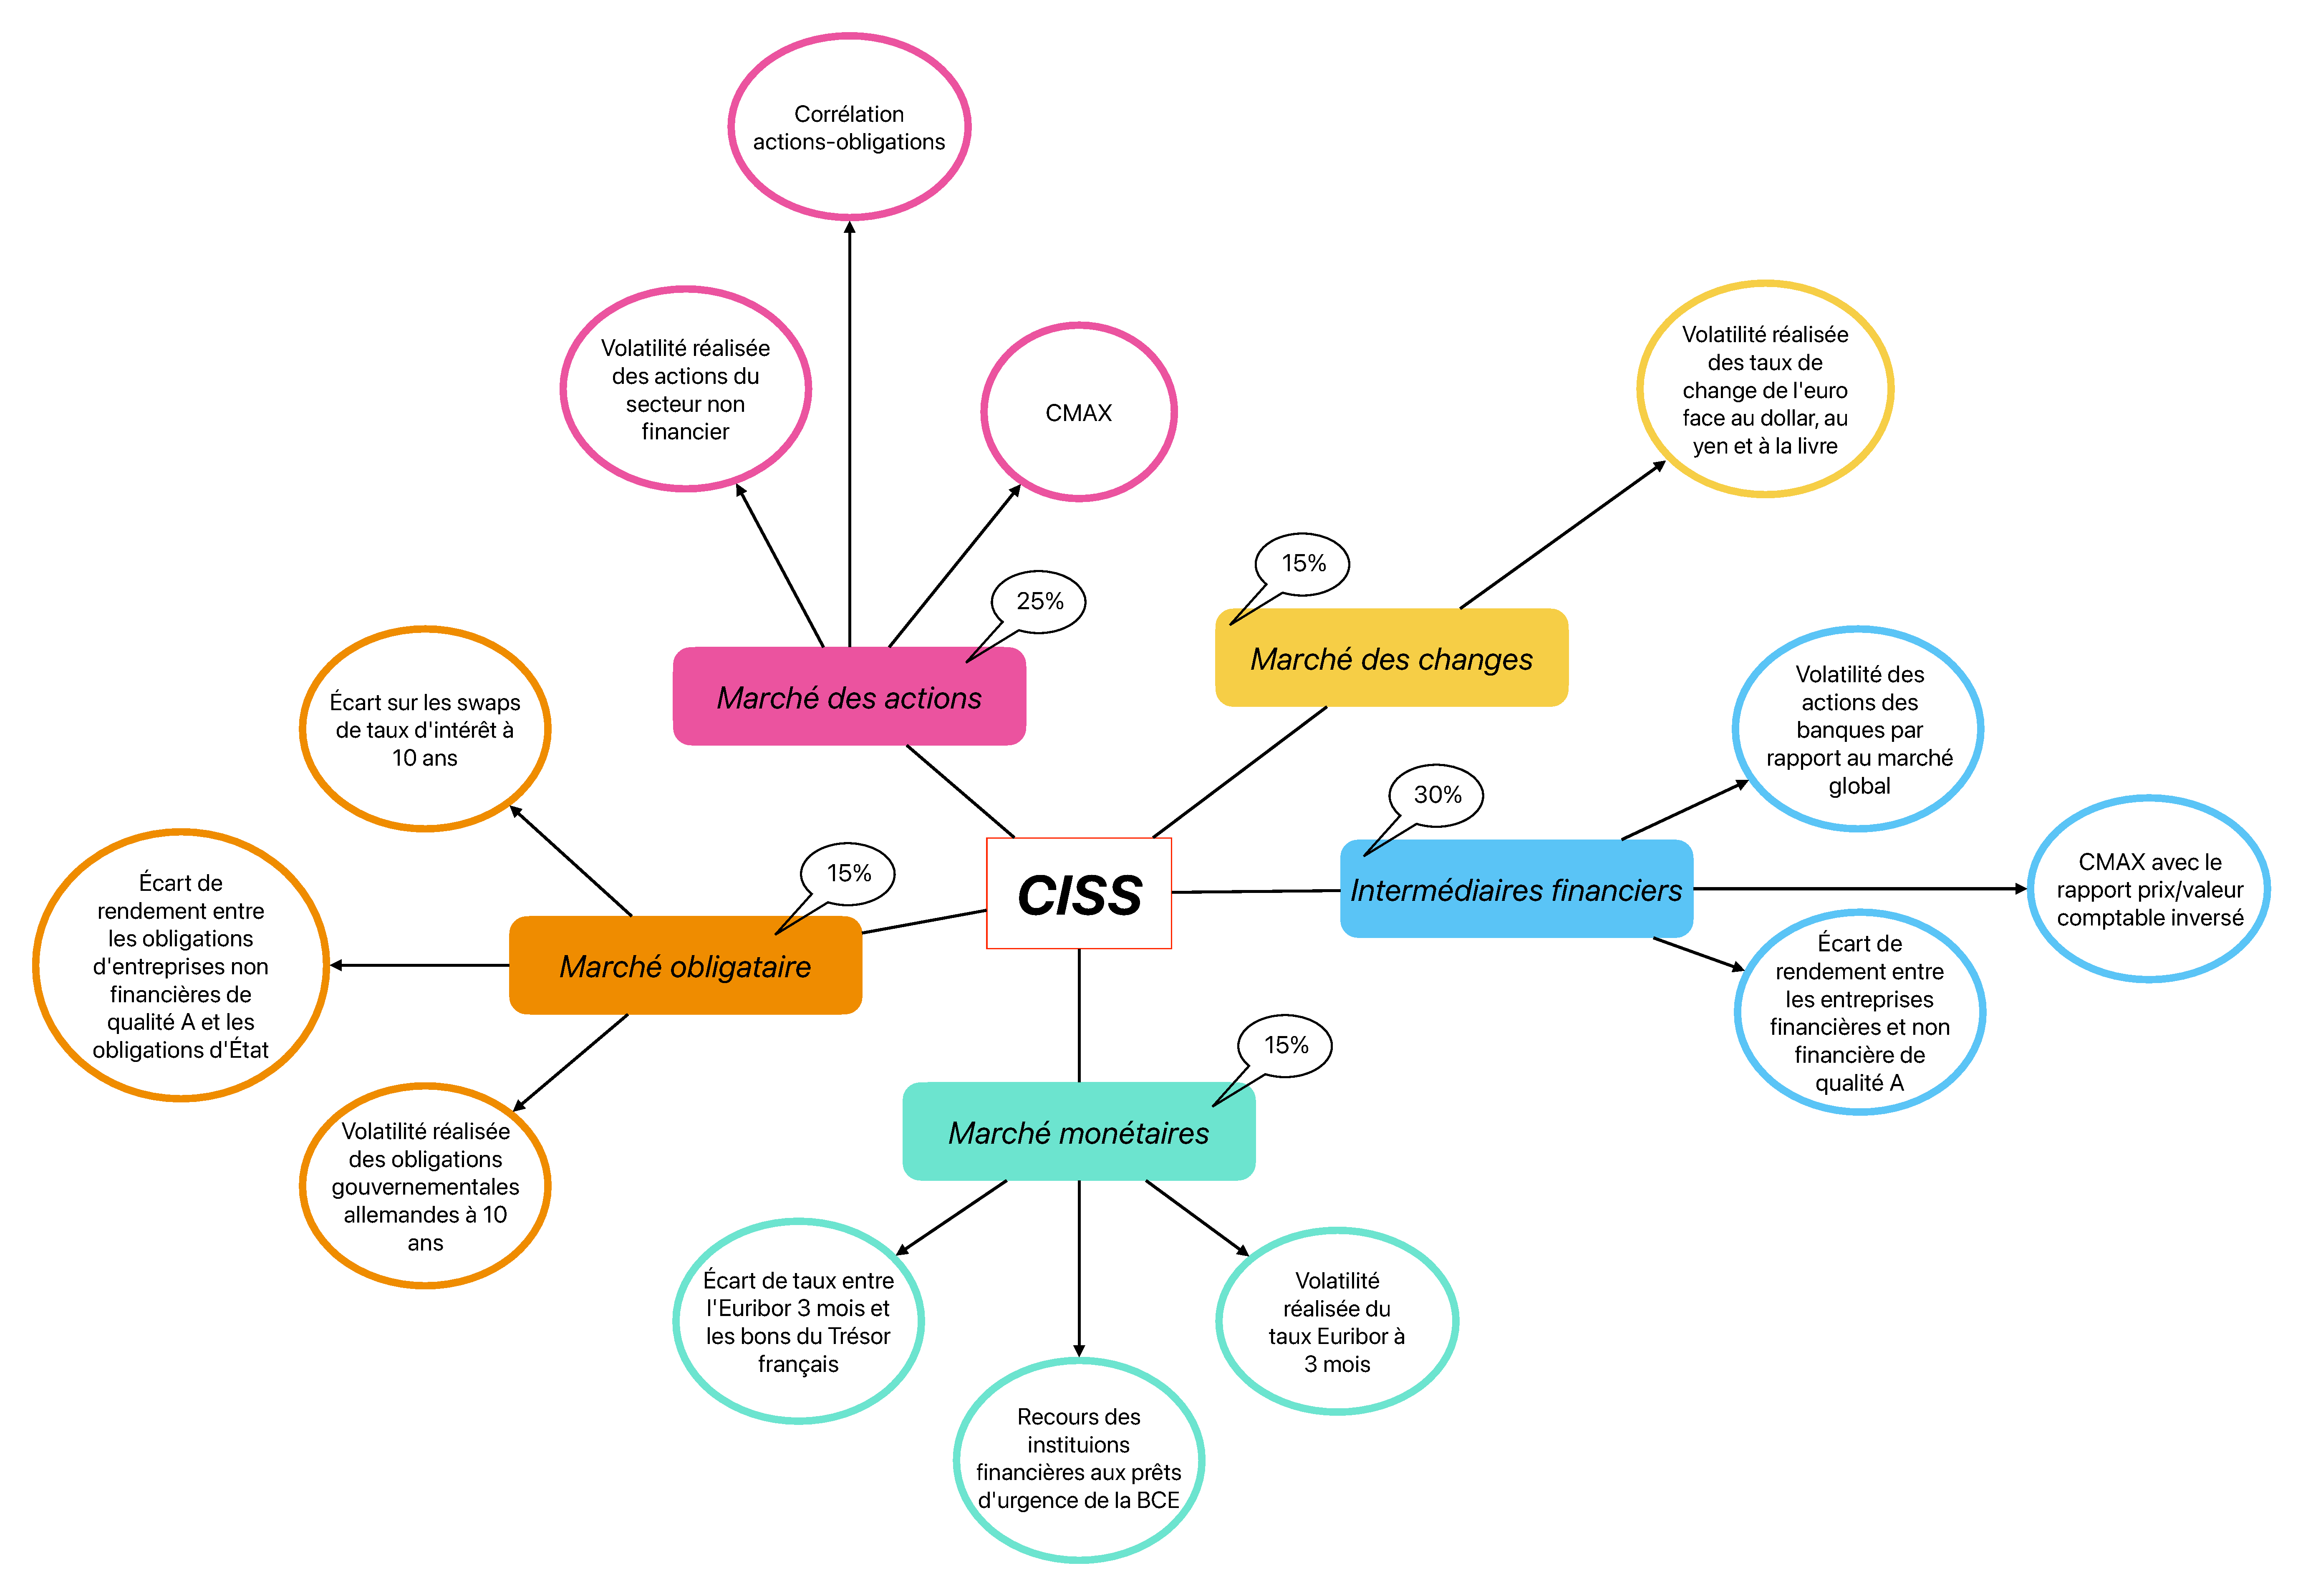
\includegraphics[width=1\linewidth]{figures/décomposition du CISS.pdf}
    \caption{Décomposition du CISS.}
    \label{fig:decomposition_ciss}
\end{sidewaysfigure}

\newpage

\section{Modélisation non-linéaire des sous indicateurs de stress systémique}\label{appendix:resultats}
\setcounter{table}{0}
\setcounter{figure}{0}

\begin{table}[H]
    \centering
    \caption{Test ARCH Forex.}
    \sffamily
    \begin{tabular}{lrrrr}
\toprule
\multicolumn{2}{l}{Heteroskedasticity Test: ARCH}&\multicolumn{1}{c}{}&\multicolumn{1}{c}{}&\multicolumn{1}{c}{}\\
[4.5pt] \hline \\ [-4.5pt]
\multicolumn{1}{l}{F-statistic}&\multicolumn{1}{r}{$267.4001$}&\multicolumn{2}{l}{Prob. F(1,225)}&\multicolumn{1}{r}{$0.0000$}\\
\multicolumn{1}{l}{Obs*R-squared}&\multicolumn{1}{r}{$123.2734$}&\multicolumn{2}{l}{Prob. Chi-Square(1)}&\multicolumn{1}{r}{$0.0000$}\\
[4.5pt] \bottomrule \\ [-4.5pt]
\end{tabular}

    \label{tab:arch_test_forex}
\end{table}

\begin{table}[H]
    \centering
    \caption{Test ARCH Equity.}
    \sffamily
    \begin{tabular}{lrrrr}
\toprule
\multicolumn{2}{l}{Heteroskedasticity Test: ARCH}&\multicolumn{1}{c}{}&\multicolumn{1}{c}{}&\multicolumn{1}{c}{}\\
[4.5pt] \hline \\ [-4.5pt]
\multicolumn{1}{l}{F-statistic}&\multicolumn{1}{r}{$209.9164$}&\multicolumn{2}{l}{Prob. F(1,225)}&\multicolumn{1}{r}{$0.0000$}\\
\multicolumn{1}{l}{Obs*R-squared}&\multicolumn{1}{r}{$109.5636$}&\multicolumn{2}{l}{Prob. Chi-Square(1)}&\multicolumn{1}{r}{$0.0000$}\\
[4.5pt] \bottomrule \\ [-4.5pt]
\end{tabular}

    \label{tab:arch_test_equity}
\end{table}

\begin{table}[H]
    \centering
    \caption{Test ARCH Imm.}
    \sffamily
    \begin{tabular}{lrrrr}
\toprule
\multicolumn{2}{l}{Heteroskedasticity Test: ARCH}&\multicolumn{1}{c}{}&\multicolumn{1}{c}{}&\multicolumn{1}{c}{}\\
[4.5pt] \hline \\ [-4.5pt]
\multicolumn{1}{l}{F-statistic}&\multicolumn{1}{r}{$484.0074$}&\multicolumn{2}{l}{Prob. F(1,225)}&\multicolumn{1}{r}{$0.0000$}\\
\multicolumn{1}{l}{Obs*R-squared}&\multicolumn{1}{r}{$154.9627$}&\multicolumn{2}{l}{Prob. Chi-Square(1)}&\multicolumn{1}{r}{$0.0000$}\\
[4.5pt] \bottomrule \\ 
\end{tabular}

    \label{tab:arch_test_imm}
\end{table}

\begin{figure}[H]
    \centering
    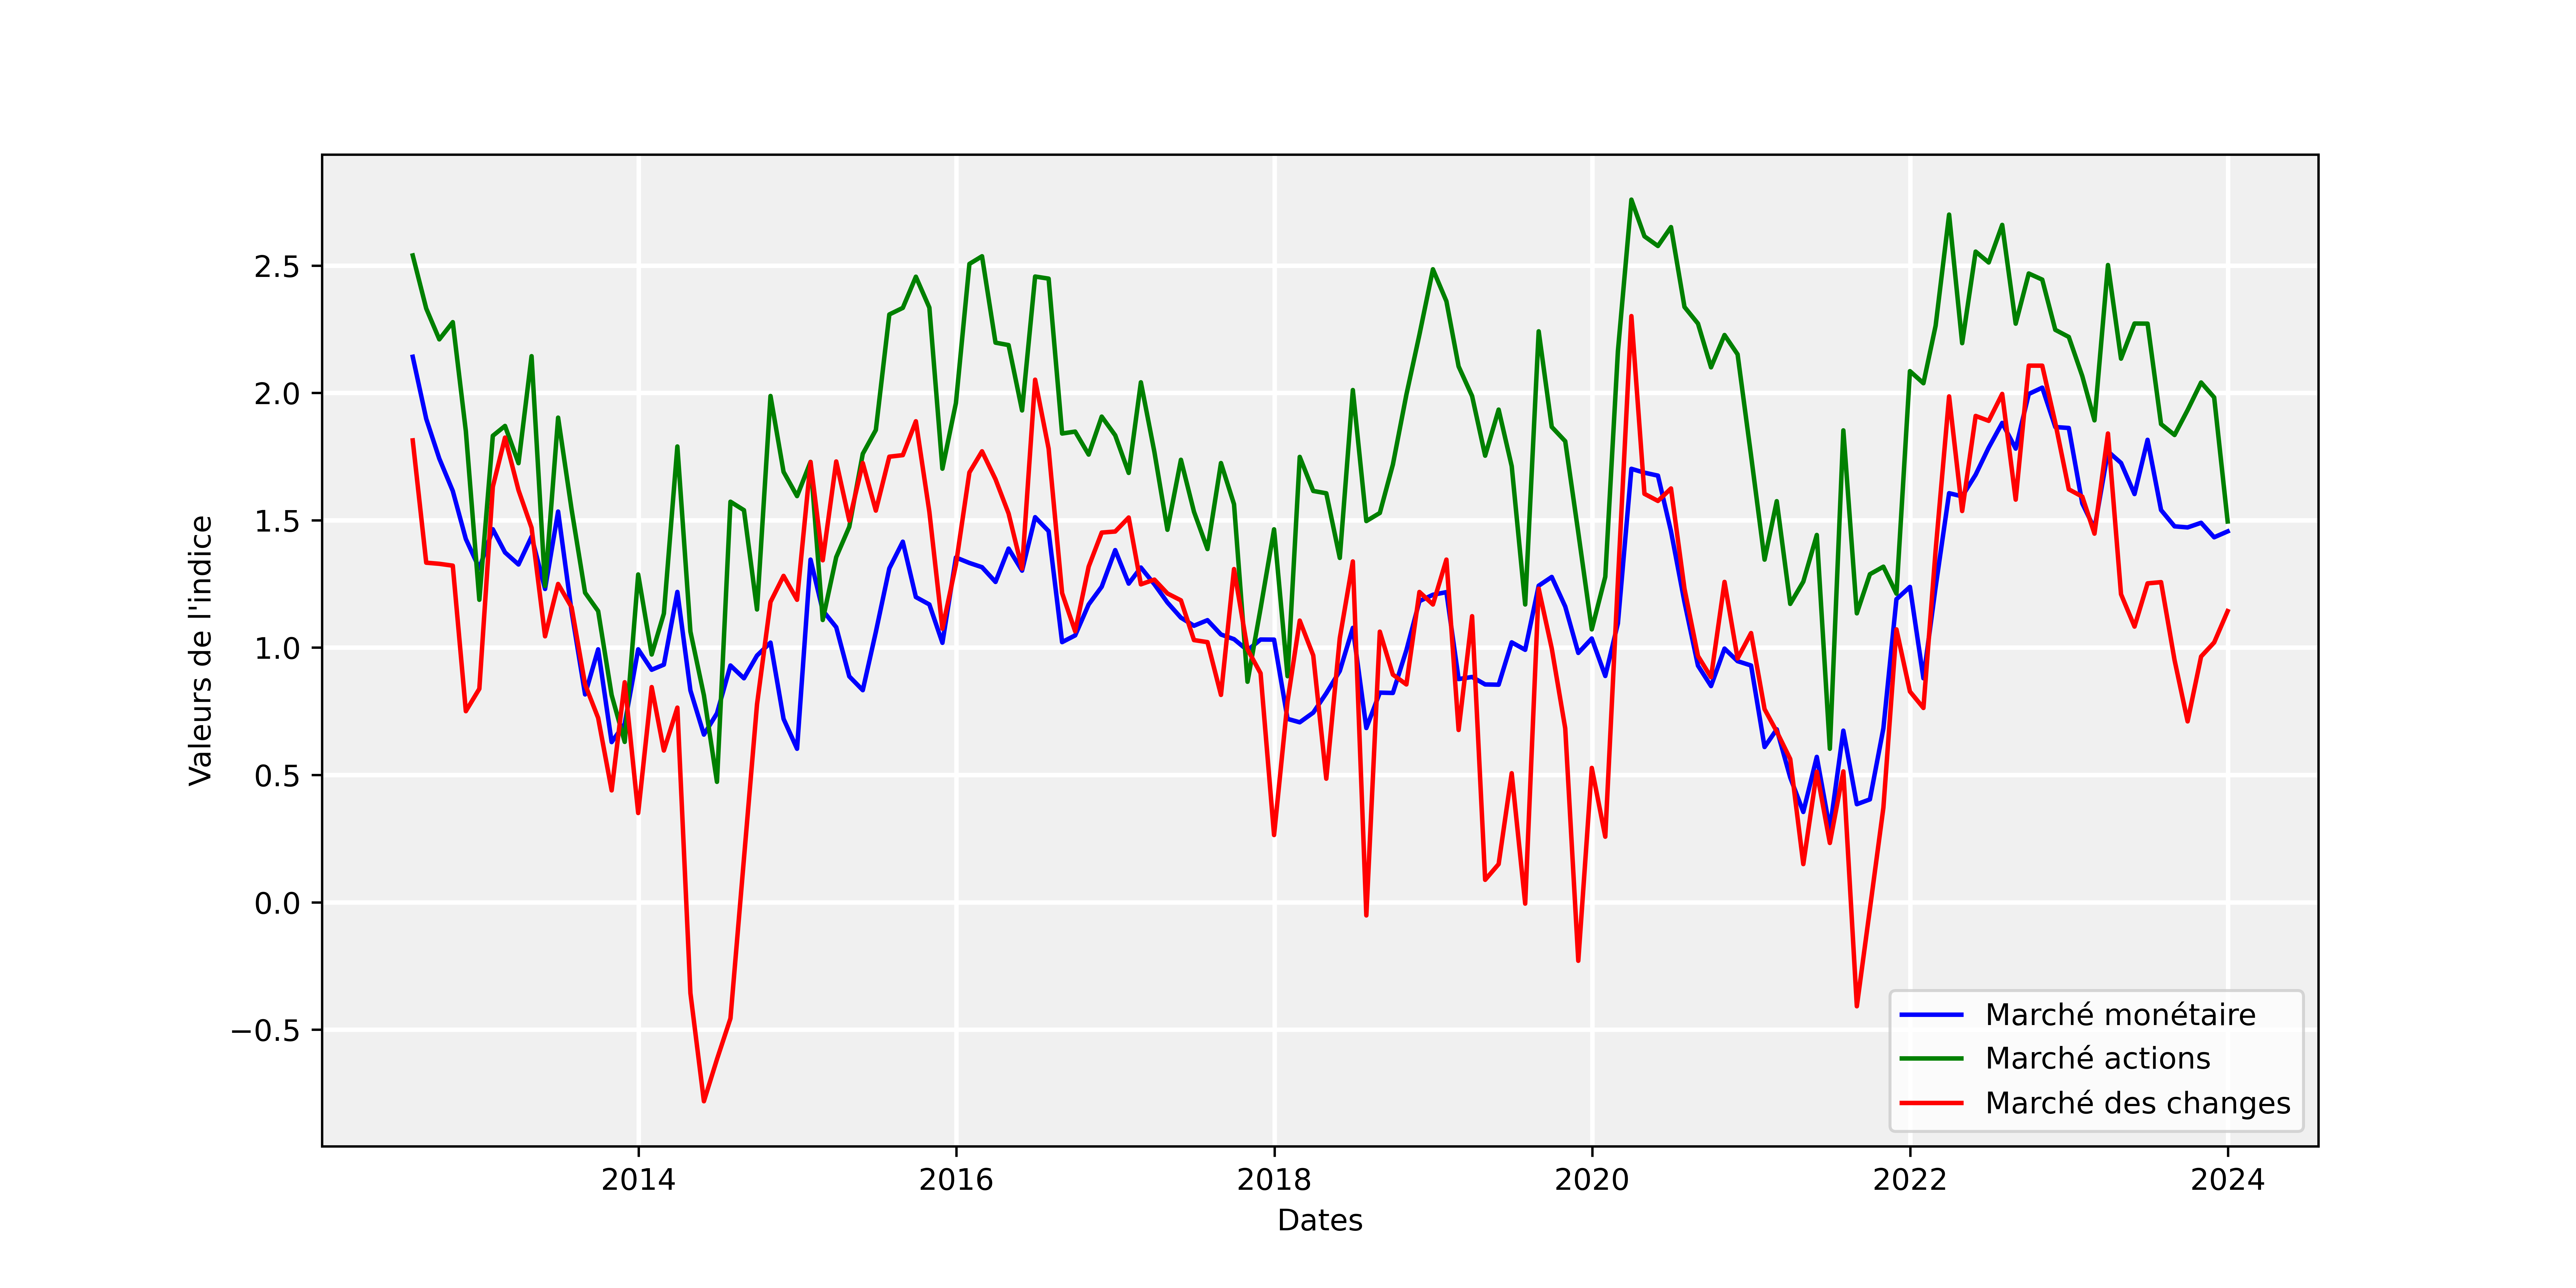
\includegraphics[width=1\linewidth]{annexes/sous_indicateurs_stress_log.png}
    \caption{Sous-indicateurs de stress en logarithme entre janvier 2005 et décembre 2024.}
    \label{fig:graphindicateurslog}
\end{figure}

\begin{figure}[H]
    \centering
    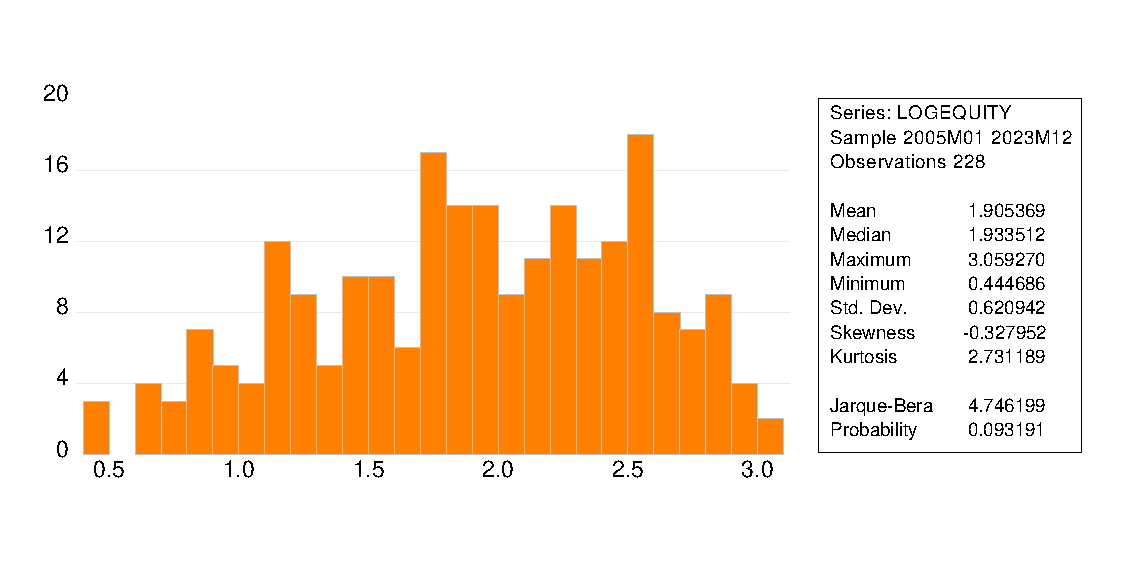
\includegraphics[width=1\linewidth]{annexes/jb_logequity.pdf}
    \caption{Test de normalité sur la série logequity.}
    \label{fig:normalitelogequity}
\end{figure}

\begin{figure}[H]
    \centering
    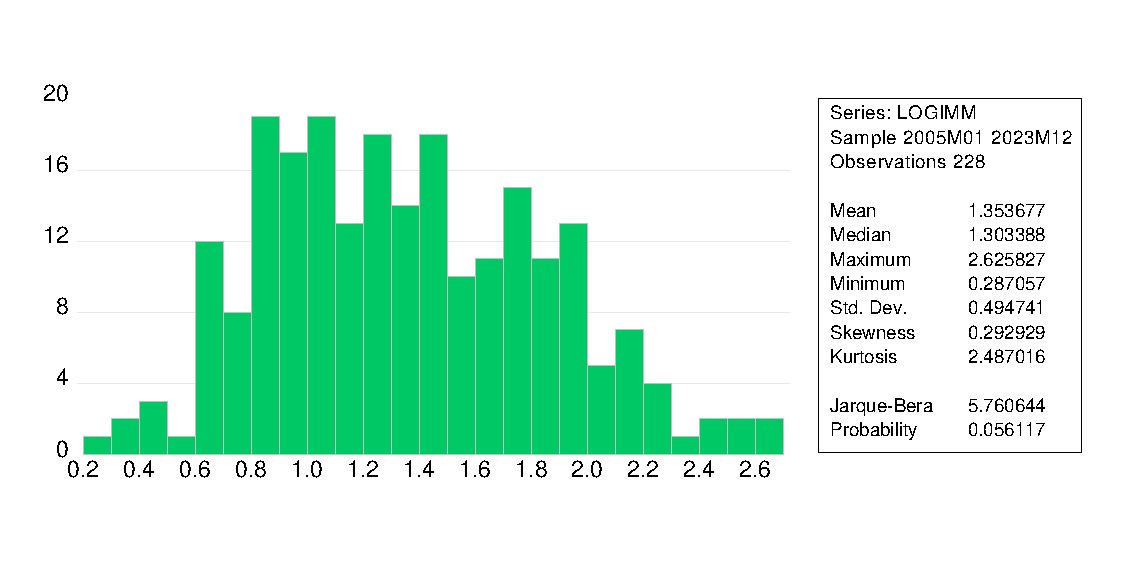
\includegraphics[width=1\linewidth]{annexes/jb_logimm.pdf}
    \caption{Test de normalité sur la série logimm.}
    \label{fig:normalitelogimm}
\end{figure}

\begin{figure}[H]
    \centering
    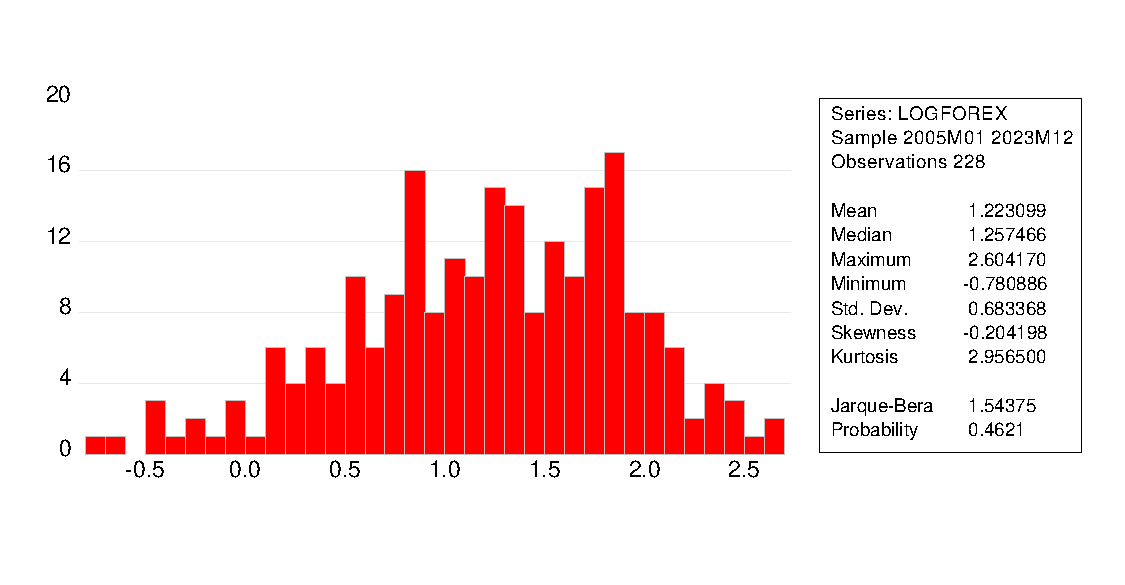
\includegraphics[width=1\linewidth]{annexes/jb_logforex.pdf}
    \caption{Test de normalité sur la série logforex.}
    \label{fig:normalitelogforex}
\end{figure}

\subsection{Détection de la saisonnalité et de la tendance}

\subsubsection*{Tests de Fischer}\label{appendix:fischer_test}

\begin{table}[H]
    \centering
    \caption[test]{Analyse de la variance}
    \sffamily 
    \resizebox{\textwidth}{!}{\begin{tabular}{lccl}
        \toprule
        Somme des carrés & Degré de liberté & Désignation & Variance\\
        \midrule
        $S_{p} = N \sum\limits_{j}(x_{\cdot j}- x_{\cdot \cdot})^2$ & $p-1$ & Variance Période & $V_{p} = \frac{S_{p}}{p-1}$ \\
        $S_{A} = P \sum\limits_{i}(x_{i \cdot}- x_{\cdot \cdot})^2$ & $N-1$ & Variance Année & $V_{A} = \frac{S_{A}}{N-1}$ \\
        $S_{R} = \sum_{i} \sum\limits_{j}(x_{ij}-x_{i\cdot}-x_{\cdot j} + x_{\cdot \cdot})^2$ & $(p-1)(N-1)$ & Variance Résidu & $V_{R} = \frac{S_{R}}{(p-1)(N-1)}$ \\
        $S_{T} $ & $N\times p-1$ & Variance Totale & $V_{T} = \frac{S_{T}}{N\times p-1}$ \\
        \bottomrule
\end{tabular}}
    \label{tab:anova}
\end{table}

\begin{table}[H]
    \centering
    \caption{Analyse de la variance du marché actions (equity)}
    \sffamily
    \begin{tabular}{rrrr}
\toprule
    \textbf{Somme des carrés} & \textbf{Degrés de liberté} & \textbf{Désignation} & \textbf{Variance} \\
\midrule
   109,92 & 11 & Variance période &  9,99 \\ 
   5643,99 & 17  & Variance année & 332,00  \\ 
   1519,97 & 187 & Variance résidus &  8,13 \\ 
\bottomrule 
\end{tabular}
    \label{tab:anova_equity}
\end{table}

\begin{table}[H]
    \centering
    \caption{Analyse de la variance du marché des changes (forex)}
    \sffamily
    \begin{tabular}{rrrr}
\toprule
    \textbf{Somme des carrés} & \textbf{Degrés de liberté} & \textbf{Désignation} & \textbf{Variance} \\
\midrule
    36,16 & 11 & Variance période &  3,29 \\ 
    1747,29 & 17  & Variance année & 102,78  \\ 
   513,47  & 187 & Variance résidus &  2,75 \\ 
\bottomrule 
\end{tabular}
    \label{tab:anova_forex}
\end{table}

\begin{table}[H]
    \centering
    \caption{Analyse de la variance du marché interbancaire (imm)}
    \sffamily
    \begin{tabular}{rrrr}
\toprule
    \textbf{Somme des carrés} & \textbf{Degrés de liberté} & \textbf{Désignation} & \textbf{Variance} \\
\midrule
    18,77 & 11 & Variance période &  1,71 \\ 
    1633,77 & 17  & Variance année & 96,10  \\ 
   395,93  & 187 & Variance résidus &  2,12 \\ 
\bottomrule 
\end{tabular}
    \label{tab:anova_imm}
\end{table}

\subsubsection*{Buys-Ballot}

\begin{table}[H]
    \centering
    \caption{Tableau de Buys-Ballot pour le marché des changes (forex)}
    \sffamily
    \resizebox{1\textwidth}{!}{\renewcommand{\arraystretch}{1.3} % pour augmenter l'espacement vertical
\begin{tabular}{|l|l|l|l|l|l|l|l|l|l|l|l|l|l|l|}
    \hline
    \textbf{années} & \textbf{janvier} & \textbf{février} & \textbf{mars} & \textbf{avril} & \textbf{mai} & \textbf{juin} & \textbf{juillet} & \textbf{août} & \textbf{septembre} & \textbf{octobre} & \textbf{novembre} & \textbf{décembre} & \textbf{$\bm{x}_{i.}$} & \textbf{$\bm{\sigma}_{i.}$} \\ \hline
    \textbf{2005} & 2,00 & 1,36 & 1,48 & 1,78 & 1,68 & 3,78 & 2,47 & 1,48 & 1,32 & 2,33 & 2,30 & 1,72 & 1,98 & 0,66 \\ \hline
    \textbf{2006} & 2,37 & 1,81 & 2,39 & 2,36 & 3,17 & 2,03 & 2,01 & 1,19 & 1,84 & 0,81 & 1,13 & 0,88 & 1,83 & 0,68 \\ \hline
    \textbf{2007} & 1,58 & 1,50 & 3,19 & 1,20 & 0,64 & 1,42 & 2,26 & 5,59 & 4,29 & 3,45 & 6,29 & 5,84 & 3,10 & 1,90 \\ \hline
    \textbf{2008} & 7,83 & 4,79 & 8,40 & 7,40 & 4,72 & 5,95 & 4,24 & 7,14 & 9,94 & 13,52 & 13,48 & 10,99 & 8,20 & 3,07 \\ \hline
    \textbf{2009} & 12,24 & 11,75 & 11,54 & 10,75 & 9,92 & 10,11 & 7,74 & 6,45 & 4,88 & 6,50 & 6,41 & 4,96 & 8,61 & 2,62 \\ \hline
    \textbf{2010} & 6,00 & 6,53 & 5,52 & 6,63 & 11,83 & 7,19 & 7,02 & 6,26 & 7,88 & 6,54 & 6,95 & 5,33 & 6,97 & 1,61 \\ \hline
    \textbf{2011} & 6,66 & 4,45 & 5,60 & 5,97 & 6,77 & 6,56 & 7,48 & 8,42 & 8,64 & 8,86 & 7,63 & 4,02 & 6,76 & 1,50 \\ \hline
    \textbf{2012} & 7,78 & 5,68 & 4,54 & 3,98 & 4,99 & 6,57 & 6,13 & 3,79 & 3,78 & 3,75 & 2,12 & 2,31 & 4,62 & 1,62 \\ \hline
    \textbf{2013} & 5,11 & 6,20 & 5,04 & 4,35 & 2,84 & 3,49 & 3,19 & 2,35 & 2,06 & 1,55 & 2,37 & 1,42 & 3,33 & 1,47 \\ \hline
    \textbf{2014} & 2,33 & 1,82 & 2,15 & 0,70 & 0,46 & 0,54 & 0,63 & 1,19 & 2,18 & 3,25 & 3,60 & 3,28 & 1,84 & 1,10 \\ \hline
    \textbf{2015} & 5,63 & 3,83 & 5,65 & 4,48 & 5,61 & 4,66 & 5,75 & 5,79 & 6,61 & 4,63 & 2,93 & 3,76 & 4,94 & 1,03 \\ \hline
    \textbf{2016} & 5,41 & 5,88 & 5,26 & 4,60 & 3,71 & 7,78 & 5,94 & 3,37 & 2,90 & 3,74 & 4,27 & 4,29 & 4,76 & 1,31 \\ \hline
    \textbf{2017} & 4,53 & 3,49 & 3,55 & 3,36 & 3,27 & 2,80 & 2,78 & 2,26 & 3,70 & 2,70 & 2,46 & 1,30 & 3,02 & 0,79 \\ \hline
    \textbf{2018} & 2,20 & 3,02 & 2,64 & 1,63 & 2,82 & 3,81 & 0,95 & 2,89 & 2,45 & 2,35 & 3,38 & 3,22 & 2,61 & 0,75 \\ \hline
    \textbf{2019} & 3,84 & 1,97 & 3,08 & 1,09 & 1,16 & 1,66 & 1,00 & 3,43 & 2,71 & 1,98 & 0,80 & 1,70 & 2,03 & 0,97 \\ \hline
    \textbf{2020} & 1,29 & 3,53 & 9,99 & 4,97 & 4,84 & 5,08 & 3,42 & 2,63 & 2,42 & 3,52 & 2,61 & 2,88 & 3,93 & 2,13 \\ \hline
    \textbf{2021} & 2,14 & 1,96 & 1,76 & 1,16 & 1,67 & 1,26 & 1,67 & 0,67 & 0,97 & 1,45 & 2,92 & 2,29 & 1,66 & 0,59 \\ \hline
    \textbf{2022} & 2,15 & 3,98 & 7,29 & 4,65 & 6,75 & 6,62 & 7,36 & 4,86 & 8,22 & 8,22 & 6,57 & 5,06 & 5,98 & 1,77 \\ \hline
    \textbf{2023} & 4,92 & 4,25 & 6,30 & 3,35 & 2,95 & 3,50 & 3,52 & 2,59 & 2,04 & 2,63 & 2,77 & 3,14 & 3,50 & 1,12 \\ \hline
    \textbf{$\bm{x}_{.j}$} & 4,53 & 4,09 & 5,02 & 3,92 & 4,20 & 4,46 & 3,98 & 3,81 & 4,15 & 4,30 & 4,26 & 3,60 & $\bm{x}_{..}$ & $\bm{\sigma}_{..}$ \\ \hline
    \textbf{$\bm{\sigma}_{.j}$} & 2,74 & 2,42 & 2,72 & 2,50 & 2,93 & 2,52 & 2,35 & 2,19 & 2,68 & 3,08 & 2,94 & 2,25 & 3,46 & 2,88 \\ \hline
\end{tabular}
}
    \label{tab:bb_forex}
\end{table}

\begin{table}[H]
    \centering
    \caption{Tableau de Buys-Ballot pour le marché interbancaire (imm)}
    \sffamily
    \resizebox{1\textwidth}{!}{\renewcommand{\arraystretch}{1.3} % pour augmenter l'espacement vertical
\begin{tabular}{|l|l|l|l|l|l|l|l|l|l|l|l|l|l|l|}
    \hline
    \textbf{années} & \textbf{janvier} & \textbf{février} & \textbf{mars} & \textbf{avril} & \textbf{mai} & \textbf{juin} & \textbf{juillet} & \textbf{août} & \textbf{septembre} & \textbf{octobre} & \textbf{novembre} & \textbf{décembre} & \textbf{$\bm{x}_{i.}$} & \textbf{$\bm{\sigma}_{i.}$} \\ \hline
    \textbf{2005} & 1,89 & 1,94 & 1,87 & 2,44 & 2,07 & 2,67 & 2,07 & 1,50 & 1,89 & 2,94 & 3,47 & 2,42 & 2,26 & 0,53 \\ \hline
    \textbf{2006} & 2,98 & 2,85 & 3,09 & 3,63 & 4,34 & 4,25 & 4,48 & 3,69 & 3,87 & 3,39 & 2,82 & 2,72 & 3,51 & 0,60 \\ \hline
    \textbf{2007} & 2,44 & 2,38 & 3,52 & 4,53 & 3,54 & 3,35 & 4,27 & 7,74 & 6,80 & 5,82 & 6,82 & 7,99 & 4,93 & 1,93 \\ \hline
    \textbf{2008} & 8,52 & 6,64 & 9,19 & 6,49 & 5,12 & 6,74 & 5,20 & 4,76 & 8,41 & 13,82 & 13,74 & 12,54 & 8,43 & 3,15 \\ \hline
    \textbf{2009} & 12,53 & 11,53 & 11,46 & 9,07 & 7,27 & 9,56 & 7,85 & 6,26 & 5,57 & 5,68 & 5,63 & 4,74 & 8,10 & 2,57 \\ \hline
    \textbf{2010} & 5,08 & 5,21 & 4,61 & 4,42 & 6,96 & 6,49 & 6,84 & 5,59 & 6,41 & 6,85 & 6,15 & 5,51 & 5,84 & 0,86 \\ \hline
    \textbf{2011} & 4,29 & 5,48 & 6,78 & 5,97 & 4,47 & 5,47 & 5,63 & 7,88 & 7,18 & 9,01 & 9,73 & 8,86 & 6,73 & 1,74 \\ \hline
    \textbf{2012} & 10,22 & 8,34 & 8,38 & 7,13 & 7,03 & 6,88 & 8,52 & 6,67 & 5,71 & 5,03 & 4,16 & 3,71 & 6,81 & 1,84 \\ \hline
    \textbf{2013} & 4,33 & 3,95 & 3,77 & 4,20 & 3,42 & 4,64 & 3,13 & 2,26 & 2,70 & 1,88 & 2,02 & 2,70 & 3,25 & 0,90 \\ \hline
    \textbf{2014} & 2,49 & 2,54 & 3,38 & 2,30 & 1,93 & 2,10 & 2,53 & 2,41 & 2,64 & 2,77 & 2,06 & 1,83 & 2,42 & 0,41 \\ \hline
    \textbf{2015} & 3,84 & 3,15 & 2,95 & 2,43 & 2,30 & 2,89 & 3,71 & 4,12 & 3,32 & 3,22 & 2,77 & 3,87 & 3,21 & 0,56 \\ \hline
    \textbf{2016} & 3,79 & 3,73 & 3,52 & 4,01 & 3,68 & 4,54 & 4,30 & 2,78 & 2,85 & 3,22 & 3,45 & 3,99 & 3,65 & 0,51 \\ \hline
    \textbf{2017} & 3,50 & 3,72 & 3,49 & 3,25 & 3,06 & 2,96 & 3,03 & 2,86 & 2,81 & 2,69 & 2,81 & 2,81 & 3,08 & 0,32 \\ \hline
    \textbf{2018} & 2,06 & 2,03 & 2,11 & 2,27 & 2,48 & 2,94 & 1,98 & 2,28 & 2,28 & 2,69 & 3,26 & 3,35 & 2,48 & 0,46 \\ \hline
    \textbf{2019} & 3,38 & 2,40 & 2,42 & 2,35 & 2,35 & 2,78 & 2,70 & 3,47 & 3,59 & 3,19 & 2,66 & 2,82 & 2,84 & 0,43 \\ \hline
    \textbf{2020} & 2,43 & 2,99 & 5,49 & 5,40 & 5,34 & 4,29 & 3,25 & 2,53 & 2,34 & 2,71 & 2,58 & 2,53 & 3,49 & 1,22 \\ \hline
    \textbf{2021} & 1,84 & 1,97 & 1,63 & 1,43 & 1,77 & 1,33 & 1,96 & 1,47 & 1,50 & 1,98 & 3,29 & 3,45 & 1,97 & 0,66 \\ \hline
    \textbf{2022} & 2,41 & 3,45 & 4,98 & 4,92 & 5,36 & 5,96 & 6,57 & 5,94 & 7,36 & 7,54 & 6,46 & 6,44 & 5,62 & 1,45 \\ \hline
    \textbf{2023} & 4,79 & 4,34 & 5,87 & 5,61 & 4,97 & 6,15 & 4,67 & 4,38 & 4,36 & 4,44 & 4,19 & 4,29 & 4,84 & 0,65 \\ \hline
    \textbf{$\bm{x}_{.j}$} & 4,36 & 4,14 & 4,66 & 4,31 & 4,08 & 4,53 & 4,35 & 4,14 & 4,29 & 4,68 & 4,64 & 4,56 & $\bm{x}_{..}$ & $\bm{\sigma}_{..}$ \\ \hline
    \textbf{$\bm{\sigma}_{.j}$} & 2,86 & 2,39 & 2,59 & 1,93 & 1,73 & 2,01 & 1,93 & 1,98 & 2,07 & 2,90 & 2,89 & 2,63 & 3,63 & 2,72 \\ \hline
\end{tabular}
}
    \label{tab:bb_imm}
\end{table}

\begin{table}[H]
    \centering
    \caption{Tableau de Buys-Ballot pour le marché actions (equity)}
    \sffamily
    \resizebox{1\textwidth}{!}{\renewcommand{\arraystretch}{1.3} % pour augmenter l'espacement vertical
\begin{tabular}{|l|l|l|l|l|l|l|l|l|l|l|l|l|l|l|}
    \hline
    \textbf{années} & \textbf{janvier} & \textbf{février} & \textbf{mars} & \textbf{avril} & \textbf{mai} & \textbf{juin} & \textbf{juillet} & \textbf{août} & \textbf{septembre} & \textbf{octobre} & \textbf{novembre} & \textbf{décembre}& \textbf{$\bm{x}_{i.}$} & \textbf{$\bm{\sigma}_{i.}$} \\ \hline
    \textbf{2005} & \hspace{3pt}1,56 & 2,16 & 2,01 & 3,62 & 3,41 & 2,42 & 2,52 & 2,26 & 2,18 & 4,77 & 3,21 & 1,57 & 2,64 & 0,90 \\ \hline
    \textbf{2006} & 2,96 & 2,71 & 2,72 & 2,79 & 6,09 & 7,74 & 7,05 & 4,22 & 4,10 & 2,41 & 3,08 & 3,18 & 4,09 & 1,77 \\ \hline
    \textbf{2007} & 2,15 & 1,86 & 7,52 & 4,34 & 2,61 & 4,65 & 7,32 & 14,35 & 12,33 & 8,02 & 12,02 & 10,43 & 7,30 & 4,10 \\ \hline
    \textbf{2008} & 15,72 & 16,02 & 17,89 & 15,30 & 11,46 & 14,48 & 12,90 & 13,27 & 18,81 & 21,31 & 20,16 & 16,56 & 16,16 & 2,85 \\ \hline
    \textbf{2009} & 16,09 & 17,10 & 19,53 & 16,86 & 14,67 & 17,24 & 16,67 & 14,14 & 10,87 & 13,77 & 12,24 & 11,07 & 15,02 & 2,58 \\ \hline
    \textbf{2010} & 11,49 & 12,52 & 9,84 & 10,92 & 18,48 & 15,15 & 12,80 & 12,17 & 10,29 & 6,77 & 5,93 & 5,78 & 11,01 & 3,57 \\ \hline
    \textbf{2011} & 5,22 & 4,97 & 8,60 & 7,24 & 6,01 & 10,42 & 12,80 & 16,90 & 18,24 & 17,56 & 16,75 & 12,27 & 11,42 & 4,84 \\ \hline
    \textbf{2012} & 11,45 & 8,65 & 9,35 & 12,58 & 13,40 & 12,70 & 12,68 & 10,29 & 9,12 & 9,76 & 6,36 & 3,28 & 9,97 & 2,83 \\ \hline
    \textbf{2013} & 6,24 & 6,49 & 5,61 & 8,54 & 3,46 & 6,71 & 4,68 & 3,37 & 3,14 & 2,26 & 1,88 & 3,62 & 4,67 & 1,96 \\ \hline
    \textbf{2014} & 2,65 & 3,11 & 5,99 & 2,90 & 2,25 & 1,61 & 4,82 & 4,66 & 3,16 & 7,30 & 5,42 & 4,93 & 4,07 & 1,64 \\ \hline
    \textbf{2015} & 5,64 & 3,03 & 3,88 & 4,37 & 5,82 & 6,39 & 10,05 & 10,32 & 11,66 & 10,33 & 5,49 & 7,10 & 7,01 & 2,76 \\ \hline
    \textbf{2016} & 12,26 & 12,64 & 9,00 & 8,92 & 6,90 & 11,67 & 11,57 & 6,30 & 6,35 & 5,80 & 6,73 & 6,26 & 8,70 & 2,55 \\ \hline
    \textbf{2017} & 5,40 & 7,70 & 5,86 & 4,32 & 5,68 & 4,63 & 4,00 & 5,61 & 4,77 & 2,38 & 3,17 & 4,33 & 4,82 & 1,32 \\ \hline
    \textbf{2018} & 2,43 & 5,75 & 5,03 & 4,98 & 3,87 & 7,47 & 4,47 & 4,61 & 5,58 & 7,34 & 9,29 & 12,01 & 6,07 & 2,49 \\ \hline
    \textbf{2019} & 10,59 & 8,20 & 7,30 & 5,78 & 6,92 & 5,54 & 3,22 & 9,41 & 6,47 & 6,11 & 4,27 & 2,92 & 6,39 & 2,22 \\ \hline
    \textbf{2020} & 3,59 & 8,70 & 15,78 & 13,66 & 13,16 & 14,17 & 10,35 & 9,70 & 8,17 & 9,27 & 8,60 & 5,77 & 10,08 & 3,43 \\ \hline
    \textbf{2021} & 3,84 & 4,83 & 3,23 & 3,52 & 4,23 & 1,83 & 6,38 & 3,11 & 3,63 & 3,74 & 3,36 & 8,05 & 4,14 & 1,57 \\ \hline
    \textbf{2022} & 7,68 & 9,62 & 14,88 & 8,98 & 12,87 & 12,33 & 14,29 & 9,70 & 11,81 & 11,53 & 9,47 & 9,20 & 11,03 & 2,17 \\ \hline
    \textbf{2023} & 7,89 & 6,64 & 12,21 & 8,45 & 9,70 & 9,70 & 6,54 & 6,26 & 6,91 & 7,70 & 7,26 & 4,46 & 7,81 & 1,93 \\ \hline
    \textbf{$\bm{x}_{.j}$} & 7,10 & 7,51 & 8,75 & 7,79 & 7,95 & 8,78 & 8,69 & 8,46 & 8,29 & 8,32 & 7,61 & 6,99 & $\bm{x}_{..}$ & $\bm{\sigma}_{..}$ \\ \hline
    \textbf{$\bm{\sigma}_{.j}$} & 4,47 & 4,38 & 5,02 & 4,24 & 4,61 & 4,65 & 4,16 & 4,25 & 4,70 & 4,91 & 4,73 & 3,88 & 6,62 & 5,13 \\ \hline
\end{tabular}
}
    \label{tab:bb_equity}
\end{table}

\subsection{Analyse de la stationnarité}

\subsubsection*{Analyse du corrélogramme}\label{appendix:correlo}

\begin{figure}[H]
    \centering
    \caption{Correlogramme du forex}
     \resizebox{0.6\textwidth}{!}{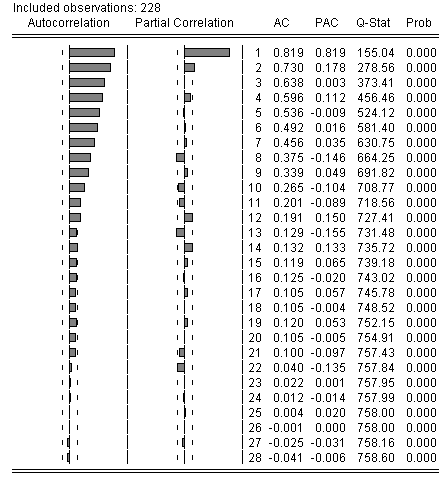
\includegraphics{annexes/correlo_logforex.png}}
    \label{tab:correlo_forex}
\end{figure}

\begin{figure}[H]
    \centering
    \caption{Correlogramme d'equity}
     \resizebox{0.6\textwidth}{!}{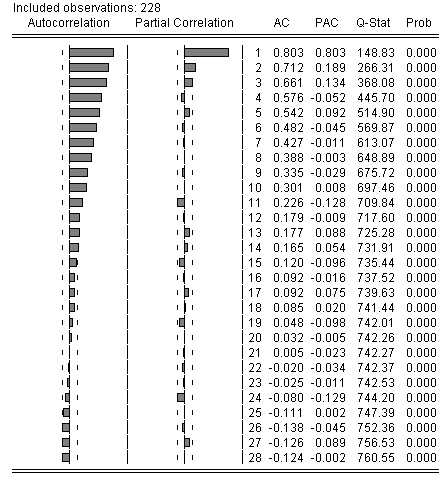
\includegraphics{annexes/correlo_logequity.png}}
    \label{tab:correlo_equity}
\end{figure}

\begin{figure}[H]
    \centering
    \caption{Correlogramme d'imm}
     \resizebox{0.6\textwidth}{!}{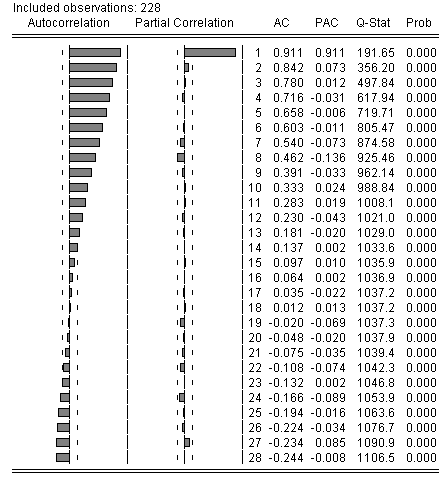
\includegraphics{annexes/correlo_logimm.png}}
    \label{tab:correlo_imm}
\end{figure}

\subsubsection*{Test de racine unitaire}

\begin{figure}[H]
    \centering
    \caption{Stratégie de Dickey-Fuller}
    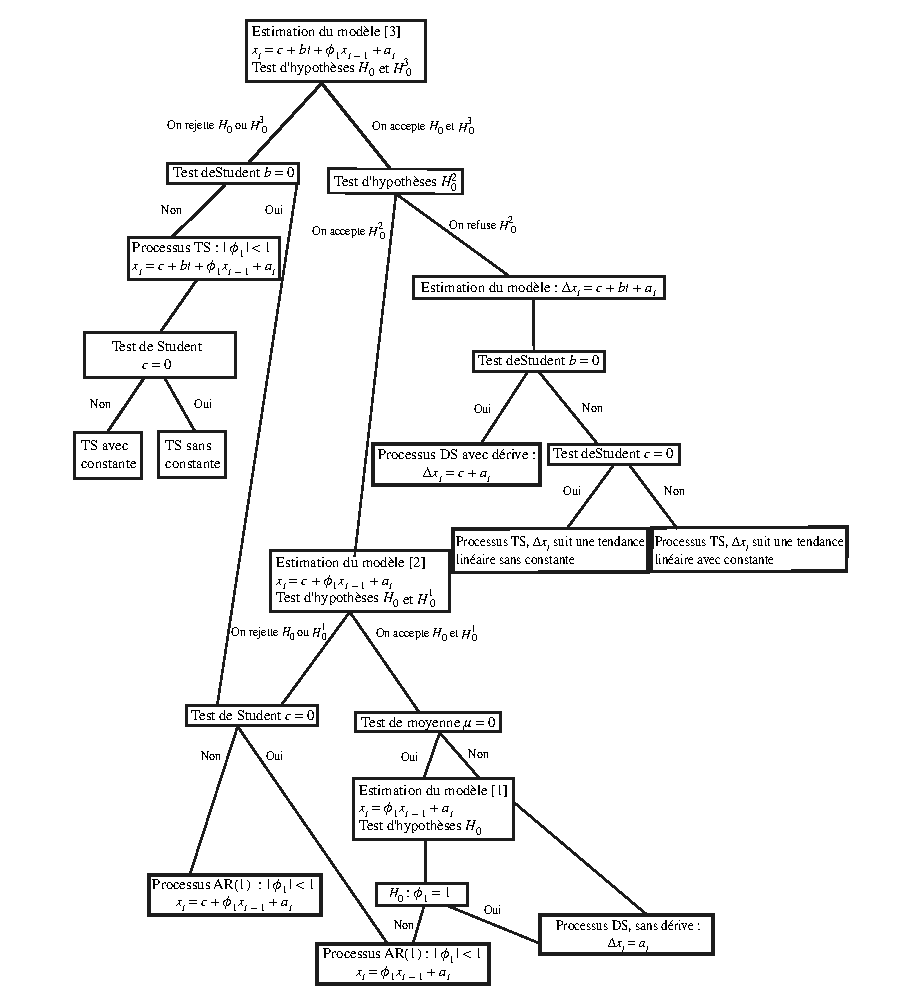
\includegraphics[scale=1.2]{annexes/df_test.pdf}
    \label{fig:strategie}
\end{figure}

\begin{figure}[H]
    \centering
    \caption{Distribution empirique de $\Phi_1$ pour $H_0^1$ (modèle 2).}
    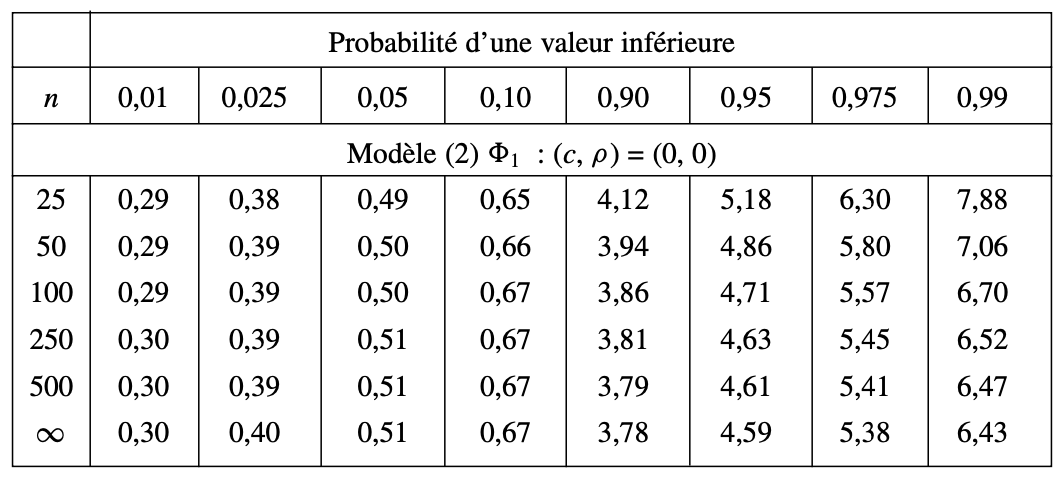
\includegraphics[scale=0.8]{annexes/dfvalues1.png}
    \label{fig:tabledf1}
\end{figure}

\begin{figure}[H]
    \centering
    \caption{Distribution empirique de $\Phi_2$ pour $H_0^2$ (modèle 3).}
    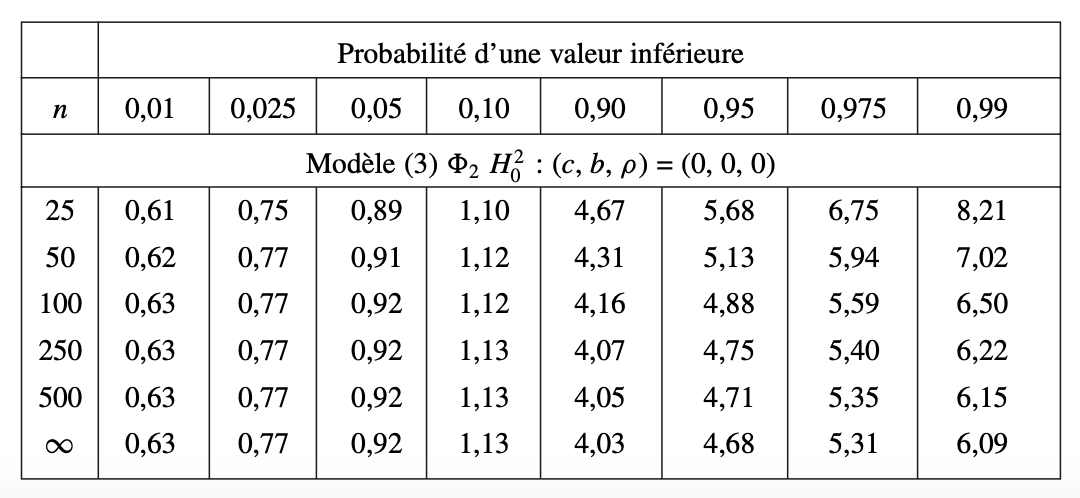
\includegraphics[scale=0.8]{annexes/dfvalues2.png}
    \label{fig:tabledf2}
\end{figure}

\begin{figure}[H]
    \centering
    \caption{Distribution empirique de $\Phi_3$ pour $H_0^3$ (modèle 3).}
    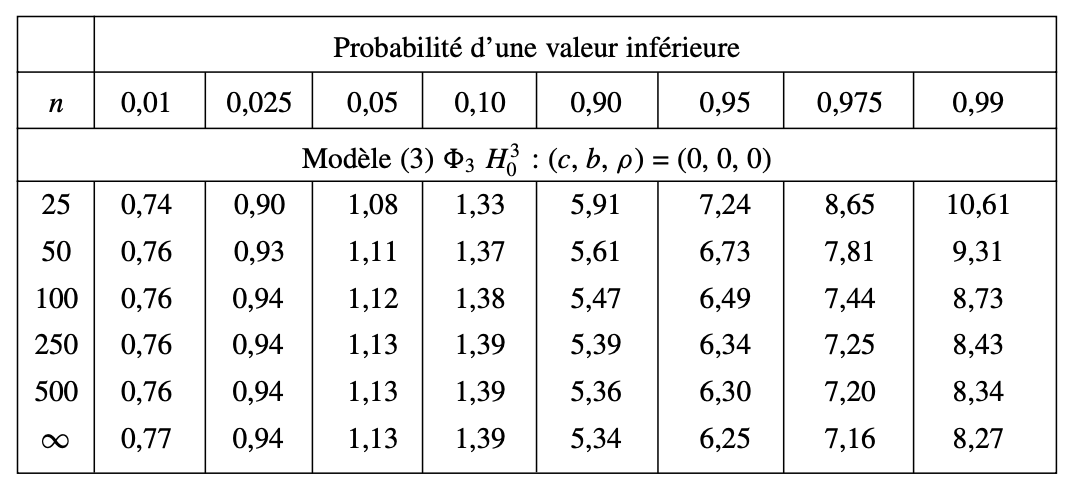
\includegraphics[scale=0.8]{annexes/dfvalues3.png}
    \label{fig:tabledf3}
\end{figure}

\begin{table}[H]
    \centering
    \caption{Estimation du modèle 3 du marché actions (equity).}
    \sffamily
    \resizebox{0.8\textwidth}{!}{\begin{tabular}{lrrrr}
\multicolumn{4}{l}{Null Hypothesis: LOGEQUITY has a unit root}&\multicolumn{1}{c}{}\\
\multicolumn{3}{l}{Exogenous: Constant, Linear Trend}&\multicolumn{1}{c}{}&\multicolumn{1}{c}{}\\
\multicolumn{5}{l}{Bandwidth: 1 (Newey-West automatic) using Bartlett kernel}\\
[4.5pt] \hline \\ [-4.5pt]
\multicolumn{1}{c}{}&\multicolumn{1}{c}{}&\multicolumn{1}{c}{}&\multicolumn{1}{c}{Adj. t-Stat}&\multicolumn{1}{c}{Prob.*}\\
[4.5pt] \hline \\ [-4.5pt]
\multicolumn{2}{l}{Phillips-Perron test statistic}&\multicolumn{1}{l}{}&\multicolumn{1}{c}{$-4.778553$}&\multicolumn{1}{c}{$0.0007$}\\
\multicolumn{1}{l}{Test critical values:}&\multicolumn{1}{c}{1\% level}&\multicolumn{1}{c}{}&\multicolumn{1}{c}{$-3.998997$}&\multicolumn{1}{c}{}\\
\multicolumn{1}{c}{}&\multicolumn{1}{c}{5\% level}&\multicolumn{1}{c}{}&\multicolumn{1}{c}{$-3.429745$}&\multicolumn{1}{c}{}\\
\multicolumn{1}{c}{}&\multicolumn{1}{c}{10\% level}&\multicolumn{1}{c}{}&\multicolumn{1}{c}{$-3.138397$}&\multicolumn{1}{c}{}\\
[4.5pt] \hline \\ [-4.5pt]
\multicolumn{2}{l}{Phillips-Perron Test Equation}&\multicolumn{1}{c}{}&\multicolumn{1}{c}{}&\multicolumn{1}{c}{}\\
\multicolumn{3}{l}{Dependent Variable: D(LOGEQUITY)}&\multicolumn{1}{c}{}&\multicolumn{1}{c}{}\\
\multicolumn{2}{l}{Method: Least Squares}&\multicolumn{1}{c}{}&\multicolumn{1}{c}{}&\multicolumn{1}{c}{}\\
\multicolumn{3}{l}{Sample (adjusted): 2005M02 2023M12}&\multicolumn{1}{c}{}&\multicolumn{1}{c}{}\\
\multicolumn{4}{l}{Included observations: 227 after adjustments}&\multicolumn{1}{c}{}\\
[4.5pt] \hline \\ [-4.5pt]
\multicolumn{1}{c}{Variable}&\multicolumn{1}{r}{Coefficient}&\multicolumn{1}{r}{Std. Error}&\multicolumn{1}{r}{t-Statistic}&\multicolumn{1}{r}{Prob.}\\
[4.5pt] \hline \\ [-4.5pt]
\multicolumn{1}{c}{LOGEQUITY(-1)}&\multicolumn{1}{r}{$-0.195158$}&\multicolumn{1}{r}{$0.038469$}&\multicolumn{1}{r}{$-5.073123$}&\multicolumn{1}{r}{$0.0000$}\\
\multicolumn{1}{c}{C}&\multicolumn{1}{r}{$0.390611$}&\multicolumn{1}{r}{$0.085740$}&\multicolumn{1}{r}{$4.555756$}&\multicolumn{1}{r}{$0.0000$}\\
\multicolumn{1}{c}{@TREND("2005M01")}&\multicolumn{1}{r}{$-0.000121$}&\multicolumn{1}{r}{$0.000364$}&\multicolumn{1}{r}{$-0.331994$}&\multicolumn{1}{r}{$0.7402$}\\
[4.5pt] \hline \\ [-4.5pt]
\multicolumn{1}{l}{R-squared}&\multicolumn{1}{r}{$0.104353$}&\multicolumn{2}{l}{Mean dependent var}&\multicolumn{1}{r}{$0.004628$}\\
\multicolumn{1}{l}{Adjusted R-squared}&\multicolumn{1}{r}{$0.096356$}&\multicolumn{2}{l}{S.D. dependent var}&\multicolumn{1}{r}{$0.377699$}\\
\multicolumn{1}{l}{S.E. of regression}&\multicolumn{1}{r}{$0.359041$}&\multicolumn{2}{l}{Akaike info criterion}&\multicolumn{1}{r}{$0.802367$}\\
\multicolumn{1}{l}{Sum squared resid}&\multicolumn{1}{r}{$28.87593$}&\multicolumn{2}{l}{Schwarz criterion}&\multicolumn{1}{r}{$0.847631$}\\
\multicolumn{1}{l}{Log likelihood}&\multicolumn{1}{r}{$-88.06867$}&\multicolumn{2}{l}{Hannan-Quinn criter.}&\multicolumn{1}{r}{$0.820632$}\\
\multicolumn{1}{l}{F-statistic}&\multicolumn{1}{r}{$13.04930$}&\multicolumn{2}{l}{Durbin-Watson stat}&\multicolumn{1}{r}{$2.312016$}\\
\multicolumn{1}{l}{Prob(F-statistic)}&\multicolumn{1}{r}{$0.000004$}&\multicolumn{1}{c}{}&\multicolumn{1}{c}{}&\multicolumn{1}{c}{}\\
[4.5pt] \hline \\ [-4.5pt]
\end{tabular}}
    \label{tab:modele3equity}
\end{table}

\begin{table}[H]
    \centering
    \caption{Estimation du modèle 3 du marché des changes (forex).}
    \sffamily
    \resizebox{0.8\textwidth}{!}{\begin{tabular}{lrrrr}
\multicolumn{4}{l}{Null Hypothesis: LOGFOREX has a unit root}&\multicolumn{1}{c}{}\\
\multicolumn{3}{l}{Exogenous: Constant, Linear Trend}&\multicolumn{1}{c}{}&\multicolumn{1}{c}{}\\
\multicolumn{5}{l}{Bandwidth: 4 (Newey-West automatic) using Bartlett kernel}\\
[4.5pt] \hline \\ [-4.5pt]
\multicolumn{1}{c}{}&\multicolumn{1}{c}{}&\multicolumn{1}{c}{}&\multicolumn{1}{c}{Adj. t-Stat}&\multicolumn{1}{c}{Prob.*}\\
[4.5pt] \hline \\ [-4.5pt]
\multicolumn{2}{l}{Phillips-Perron test statistic}&\multicolumn{1}{l}{}&\multicolumn{1}{c}{$-4.454248$}&\multicolumn{1}{c}{$0.0022$}\\
\multicolumn{1}{l}{Test critical values:}&\multicolumn{1}{c}{1\% level}&\multicolumn{1}{c}{}&\multicolumn{1}{c}{$-3.998997$}&\multicolumn{1}{c}{}\\
\multicolumn{1}{c}{}&\multicolumn{1}{c}{5\% level}&\multicolumn{1}{c}{}&\multicolumn{1}{c}{$-3.429745$}&\multicolumn{1}{c}{}\\
\multicolumn{1}{c}{}&\multicolumn{1}{c}{10\% level}&\multicolumn{1}{c}{}&\multicolumn{1}{c}{$-3.138397$}&\multicolumn{1}{c}{}\\
[4.5pt] \hline \\ [-4.5pt]
\multicolumn{2}{l}{Phillips-Perron Test Equation}&\multicolumn{1}{c}{}&\multicolumn{1}{c}{}&\multicolumn{1}{c}{}\\
\multicolumn{3}{l}{Dependent Variable: D(LOGFOREX)}&\multicolumn{1}{c}{}&\multicolumn{1}{c}{}\\
\multicolumn{2}{l}{Method: Least Squares}&\multicolumn{1}{c}{}&\multicolumn{1}{c}{}&\multicolumn{1}{c}{}\\
\multicolumn{3}{l}{Sample (adjusted): 2005M02 2023M12}&\multicolumn{1}{c}{}&\multicolumn{1}{c}{}\\
\multicolumn{4}{l}{Included observations: 227 after adjustments}&\multicolumn{1}{c}{}\\
[4.5pt] \hline \\ [-4.5pt]
\multicolumn{1}{c}{Variable}&\multicolumn{1}{r}{Coefficient}&\multicolumn{1}{r}{Std. Error}&\multicolumn{1}{r}{t-Statistic}&\multicolumn{1}{r}{Prob.}\\
[4.5pt] \hline \\ [-4.5pt]
\multicolumn{1}{c}{LOGFOREX(-1)}&\multicolumn{1}{r}{$-0.183168$}&\multicolumn{1}{r}{$0.038310$}&\multicolumn{1}{r}{$-4.781184$}&\multicolumn{1}{r}{$0.0000$}\\
\multicolumn{1}{c}{C}&\multicolumn{1}{r}{$0.255576$}&\multicolumn{1}{r}{$0.073272$}&\multicolumn{1}{r}{$3.488049$}&\multicolumn{1}{r}{$0.0006$}\\
\multicolumn{1}{c}{@TREND("2005M01")}&\multicolumn{1}{r}{$-0.000259$}&\multicolumn{1}{r}{$0.000400$}&\multicolumn{1}{r}{$-0.647636$}&\multicolumn{1}{r}{$0.5179$}\\
[4.5pt] \hline \\ [-4.5pt]
\multicolumn{1}{l}{R-squared}&\multicolumn{1}{r}{$0.092720$}&\multicolumn{2}{l}{Mean dependent var}&\multicolumn{1}{r}{$0.001984$}\\
\multicolumn{1}{l}{Adjusted R-squared}&\multicolumn{1}{r}{$0.084620$}&\multicolumn{2}{l}{S.D. dependent var}&\multicolumn{1}{r}{$0.410266$}\\
\multicolumn{1}{l}{S.E. of regression}&\multicolumn{1}{r}{$0.392524$}&\multicolumn{2}{l}{Akaike info criterion}&\multicolumn{1}{r}{$0.980692$}\\
\multicolumn{1}{l}{Sum squared resid}&\multicolumn{1}{r}{$34.51289$}&\multicolumn{2}{l}{Schwarz criterion}&\multicolumn{1}{r}{$1.025955$}\\
\multicolumn{1}{l}{Log likelihood}&\multicolumn{1}{r}{$-108.3085$}&\multicolumn{2}{l}{Hannan-Quinn criter.}&\multicolumn{1}{r}{$0.998956$}\\
\multicolumn{1}{l}{F-statistic}&\multicolumn{1}{r}{$11.44594$}&\multicolumn{2}{l}{Durbin-Watson stat}&\multicolumn{1}{r}{$2.300682$}\\
\multicolumn{1}{l}{Prob(F-statistic)}&\multicolumn{1}{r}{$0.000018$}&\multicolumn{1}{c}{}&\multicolumn{1}{c}{}&\multicolumn{1}{c}{}\\
[4.5pt] \hline \\ [-4.5pt]
\end{tabular}}
    \label{tab:modele3forex}
\end{table}

\begin{table}[H]
    \centering
    \caption{Estimation du modèle 3 du marché interbancaire (imm).}
    \sffamily
    \resizebox{0.8\textwidth}{!}{\begin{tabular}{lrrrr}
\multicolumn{3}{l}{Null Hypothesis: LOGIMM has a unit root}&\multicolumn{1}{c}{}&\multicolumn{1}{c}{}\\
\multicolumn{3}{l}{Exogenous: Constant, Linear Trend}&\multicolumn{1}{c}{}&\multicolumn{1}{c}{}\\
\multicolumn{5}{l}{Bandwidth: 4 (Newey-West automatic) using Bartlett kernel}\\
[4.5pt] \hline \\ [-4.5pt]
\multicolumn{1}{c}{}&\multicolumn{1}{c}{}&\multicolumn{1}{c}{}&\multicolumn{1}{c}{Adj. t-Stat}&\multicolumn{1}{c}{Prob.*}\\
[4.5pt] \hline \\ [-4.5pt]
\multicolumn{2}{l}{Phillips-Perron test statistic}&\multicolumn{1}{l}{}&\multicolumn{1}{c}{$-3.503584$}&\multicolumn{1}{c}{$0.0414$}\\
\multicolumn{1}{l}{Test critical values:}&\multicolumn{1}{c}{1\% level}&\multicolumn{1}{c}{}&\multicolumn{1}{c}{$-3.998997$}&\multicolumn{1}{c}{}\\
\multicolumn{1}{c}{}&\multicolumn{1}{c}{5\% level}&\multicolumn{1}{c}{}&\multicolumn{1}{c}{$-3.429745$}&\multicolumn{1}{c}{}\\
\multicolumn{1}{c}{}&\multicolumn{1}{c}{10\% level}&\multicolumn{1}{c}{}&\multicolumn{1}{c}{$-3.138397$}&\multicolumn{1}{c}{}\\
[4.5pt] \hline \\ [-4.5pt]
\multicolumn{2}{l}{Phillips-Perron Test Equation}&\multicolumn{1}{c}{}&\multicolumn{1}{c}{}&\multicolumn{1}{c}{}\\
\multicolumn{3}{l}{Dependent Variable: D(LOGIMM)}&\multicolumn{1}{c}{}&\multicolumn{1}{c}{}\\
\multicolumn{2}{l}{Method: Least Squares}&\multicolumn{1}{c}{}&\multicolumn{1}{c}{}&\multicolumn{1}{c}{}\\
\multicolumn{3}{l}{Sample (adjusted): 2005M02 2023M12}&\multicolumn{1}{c}{}&\multicolumn{1}{c}{}\\
\multicolumn{4}{l}{Included observations: 227 after adjustments}&\multicolumn{1}{c}{}\\
[4.5pt] \hline \\ [-4.5pt]
\multicolumn{1}{c}{Variable}&\multicolumn{1}{r}{Coefficient}&\multicolumn{1}{r}{Std. Error}&\multicolumn{1}{r}{t-Statistic}&\multicolumn{1}{r}{Prob.}\\
[4.5pt] \hline \\ [-4.5pt]
\multicolumn{1}{c}{LOGIMM(-1)}&\multicolumn{1}{r}{$-0.089788$}&\multicolumn{1}{r}{$0.024944$}&\multicolumn{1}{r}{$-3.599590$}&\multicolumn{1}{r}{$0.0004$}\\
\multicolumn{1}{c}{C}&\multicolumn{1}{r}{$0.144106$}&\multicolumn{1}{r}{$0.042312$}&\multicolumn{1}{r}{$3.405797$}&\multicolumn{1}{r}{$0.0008$}\\
\multicolumn{1}{c}{@TREND("2005M01")}&\multicolumn{1}{r}{$4.74E-05$}&\multicolumn{1}{r}{$0.000219$}&\multicolumn{1}{r}{$0.216505$}&\multicolumn{1}{r}{$0.8288$}\\
[4.5pt] \hline \\ [-4.5pt]
\multicolumn{1}{l}{R-squared}&\multicolumn{1}{r}{$0.057418$}&\multicolumn{2}{l}{Mean dependent var}&\multicolumn{1}{r}{$0.008931$}\\
\multicolumn{1}{l}{Adjusted R-squared}&\multicolumn{1}{r}{$0.049002$}&\multicolumn{2}{l}{S.D. dependent var}&\multicolumn{1}{r}{$0.212872$}\\
\multicolumn{1}{l}{S.E. of regression}&\multicolumn{1}{r}{$0.207591$}&\multicolumn{2}{l}{Akaike info criterion}&\multicolumn{1}{r}{$-0.293364$}\\
\multicolumn{1}{l}{Sum squared resid}&\multicolumn{1}{r}{$9.653077$}&\multicolumn{2}{l}{Schwarz criterion}&\multicolumn{1}{r}{$-0.248101$}\\
\multicolumn{1}{l}{Log likelihood}&\multicolumn{1}{r}{$36.29687$}&\multicolumn{2}{l}{Hannan-Quinn criter.}&\multicolumn{1}{r}{$-0.275100$}\\
\multicolumn{1}{l}{F-statistic}&\multicolumn{1}{r}{$6.822506$}&\multicolumn{2}{l}{Durbin-Watson stat}&\multicolumn{1}{r}{$2.196933$}\\
\multicolumn{1}{l}{Prob(F-statistic)}&\multicolumn{1}{r}{$0.001330$}&\multicolumn{1}{c}{}&\multicolumn{1}{c}{}&\multicolumn{1}{c}{}\\
[4.5pt] \hline \\ [-4.5pt]
\end{tabular}}
    \label{tab:modele3imm}
\end{table}

\subsection{Estimation du modèle MS-VAR}

\subsubsection{Choix de la forme du modèle optimale}

\begin{table}[H]
    \centering
    \sffamily
    \caption{Estimation du modèle VAR(1) linéaire standard.}
    \label{tab:modele_ms_var_lineaire}
    \resizebox{0.8\textwidth}{!}{\begin{tabular}{lrrr}
\multicolumn{2}{l}{Vector Autoregression Estimates}&\multicolumn{1}{c}{}&\multicolumn{1}{c}{}\\
\multicolumn{3}{l}{Sample (adjusted): 2005M02 2023M12}&\multicolumn{1}{c}{}\\
\multicolumn{3}{l}{Included observations: 227 after adjustments}&\multicolumn{1}{c}{}\\
\multicolumn{3}{l}{Standard errors in ( ) \& t-statistics in [ ]}&\multicolumn{1}{c}{}\\
[4.5pt] \hline \\ [-4.5pt]
\multicolumn{1}{c}{}&\multicolumn{1}{c}{LOGIMM}&\multicolumn{1}{c}{LOGFOREX}&\multicolumn{1}{c}{LOGEQUITY}\\
[4.5pt] \hline \\ [-4.5pt]
\multicolumn{1}{c}{LOGIMM(-1)}&\multicolumn{1}{c}{$0.879708$}&\multicolumn{1}{c}{$0.152680$}&\multicolumn{1}{c}{$0.131701$}\\
\multicolumn{1}{c}{}&\multicolumn{1}{c}{$(0.04897)$}&\multicolumn{1}{c}{$(0.09426)$}&\multicolumn{1}{c}{$(0.08481)$}\\
\multicolumn{1}{c}{}&\multicolumn{1}{c}{[ 17.9656]}&\multicolumn{1}{c}{[ 1.61983]}&\multicolumn{1}{c}{[ 1.55284]}\\
\multicolumn{1}{c}{}&\multicolumn{1}{c}{}&\multicolumn{1}{c}{}&\multicolumn{1}{c}{}\\
\multicolumn{1}{c}{LOGFOREX(-1)}&\multicolumn{1}{c}{$0.036506$}&\multicolumn{1}{c}{$0.699607$}&\multicolumn{1}{c}{$0.135807$}\\
\multicolumn{1}{c}{}&\multicolumn{1}{c}{$(0.03539)$}&\multicolumn{1}{c}{$(0.06812)$}&\multicolumn{1}{c}{$(0.06129)$}\\
\multicolumn{1}{c}{}&\multicolumn{1}{c}{[ 1.03159]}&\multicolumn{1}{c}{[ 10.2702]}&\multicolumn{1}{c}{[ 2.21563]}\\
\multicolumn{1}{c}{}&\multicolumn{1}{c}{}&\multicolumn{1}{c}{}&\multicolumn{1}{c}{}\\
\multicolumn{1}{c}{LOGEQUITY(-1)}&\multicolumn{1}{c}{$-0.010466$}&\multicolumn{1}{c}{$0.046203$}&\multicolumn{1}{c}{$0.602090$}\\
\multicolumn{1}{c}{}&\multicolumn{1}{c}{$(0.04001)$}&\multicolumn{1}{c}{$(0.07701)$}&\multicolumn{1}{c}{$(0.06930)$}\\
\multicolumn{1}{c}{}&\multicolumn{1}{c}{[-0.26159]}&\multicolumn{1}{c}{[ 0.59993]}&\multicolumn{1}{c}{[ 8.68842]}\\
\multicolumn{1}{c}{}&\multicolumn{1}{c}{}&\multicolumn{1}{c}{}&\multicolumn{1}{c}{}\\
\multicolumn{1}{c}{C}&\multicolumn{1}{c}{$0.141685$}&\multicolumn{1}{c}{$0.074771$}&\multicolumn{1}{c}{$0.419139$}\\
\multicolumn{1}{c}{}&\multicolumn{1}{c}{$(0.04768)$}&\multicolumn{1}{c}{$(0.09179)$}&\multicolumn{1}{c}{$(0.08259)$}\\
\multicolumn{1}{c}{}&\multicolumn{1}{c}{[ 2.97142]}&\multicolumn{1}{c}{[ 0.81463]}&\multicolumn{1}{c}{[ 5.07500]}\\
[4.5pt] \hline \\ [-4.5pt]
\multicolumn{1}{l}{R-squared}&\multicolumn{1}{c}{$0.834127$}&\multicolumn{1}{c}{$0.679987$}&\multicolumn{1}{c}{$0.679165$}\\
\multicolumn{1}{l}{Adj. R-squared}&\multicolumn{1}{c}{$0.831895$}&\multicolumn{1}{c}{$0.675682$}&\multicolumn{1}{c}{$0.674849$}\\
\multicolumn{1}{l}{Sum sq. resids}&\multicolumn{1}{c}{$9.130951$}&\multicolumn{1}{c}{$33.83337$}&\multicolumn{1}{c}{$27.39324$}\\
\multicolumn{1}{l}{S.E. equation}&\multicolumn{1}{c}{$0.202351$}&\multicolumn{1}{c}{$0.389511$}&\multicolumn{1}{c}{$0.350485$}\\
\multicolumn{1}{l}{F-statistic}&\multicolumn{1}{c}{$373.8004$}&\multicolumn{1}{c}{$157.9491$}&\multicolumn{1}{c}{$157.3536$}\\
\multicolumn{1}{l}{Log likelihood}&\multicolumn{1}{c}{$42.60825$}&\multicolumn{1}{c}{$-106.0515$}&\multicolumn{1}{c}{$-82.08586$}\\
\multicolumn{1}{l}{Akaike AIC}&\multicolumn{1}{c}{$-0.340161$}&\multicolumn{1}{c}{$0.969617$}&\multicolumn{1}{c}{$0.758466$}\\
\multicolumn{1}{l}{Schwarz SC}&\multicolumn{1}{c}{$-0.279809$}&\multicolumn{1}{c}{$1.029969$}&\multicolumn{1}{c}{$0.818817$}\\
\multicolumn{1}{l}{Mean dependent}&\multicolumn{1}{c}{$1.356830$}&\multicolumn{1}{c}{$1.225433$}&\multicolumn{1}{c}{$1.911804$}\\
\multicolumn{1}{l}{S.D. dependent}&\multicolumn{1}{c}{$0.493533$}&\multicolumn{1}{c}{$0.683967$}&\multicolumn{1}{c}{$0.614648$}\\
[4.5pt] \hline \\ [-4.5pt]
\multicolumn{2}{l}{Determinant resid covariance (dof adj.)}&\multicolumn{1}{c}{$0.000280$}&\multicolumn{1}{c}{}\\
\multicolumn{2}{l}{Determinant resid covariance}&\multicolumn{1}{c}{$0.000266$}&\multicolumn{1}{c}{}\\
\multicolumn{1}{l}{Log likelihood}&\multicolumn{1}{c}{}&\multicolumn{1}{c}{$-31.90854$}&\multicolumn{1}{c}{}\\
\multicolumn{2}{l}{Akaike information criterion}&\multicolumn{1}{c}{$0.386859$}&\multicolumn{1}{c}{}\\
\multicolumn{1}{l}{Schwarz criterion}&\multicolumn{1}{c}{}&\multicolumn{1}{c}{$0.567914$}&\multicolumn{1}{c}{}\\
\multicolumn{1}{l}{Number of coefficients}&\multicolumn{1}{c}{}&\multicolumn{1}{c}{$12$}&\multicolumn{1}{c}{}\\
[4.5pt] \hline \\ [-4.5pt]
\end{tabular}
}
\end{table}

\begin{table}[H]
    \centering
    \sffamily
    \caption{Estimation du modèle MS-VAR.}
    \label{tab:modele_ms_var}
    \resizebox{0.8\textwidth}{!}{\begin{tabular}{lrrrr}
\multicolumn{5}{l}{Markov Switching Intercepts VAR Estimates (BFGS / Marquardt steps)}\\
\multicolumn{3}{l}{Sample (adjusted): 2005M02 2023M12}&\multicolumn{1}{c}{}&\multicolumn{1}{c}{}\\
\multicolumn{3}{l}{Included observations: 227 after adjustments}&\multicolumn{1}{c}{}&\multicolumn{1}{c}{}\\
\multicolumn{1}{l}{Number of states: 2}&\multicolumn{1}{c}{}&\multicolumn{1}{c}{}&\multicolumn{1}{c}{}&\multicolumn{1}{c}{}\\
\multicolumn{4}{l}{Initial probabilities obtained from ergodic solution}&\multicolumn{1}{c}{}\\
\multicolumn{4}{l}{Huber-White robust standard errors \& covariance}&\multicolumn{1}{c}{}\\
\multicolumn{6}{l}{Random search: 25 starting values with 10 iterations using 1 standard deviation}\\
\multicolumn{2}{l}{(rng=kn, seed=1307615851)}&\multicolumn{1}{c}{}&\multicolumn{1}{c}{}&\multicolumn{1}{c}{}\\
\multicolumn{3}{l}{Convergence achieved after 85 iterations}&\multicolumn{1}{c}{}&\multicolumn{1}{c}{}\\
\multicolumn{3}{l}{Standard errors in ( ) \& z-statistics in [ ]}&\multicolumn{1}{c}{}&\multicolumn{1}{c}{}\\
[4.5pt] \hline \\ [-4.5pt]
\multicolumn{1}{c}{}&\multicolumn{1}{c}{LOGFOREX}&\multicolumn{1}{c}{LOGIMM}&\multicolumn{1}{c}{LOGEQUITY}&\multicolumn{1}{c}{}\\
[4.5pt] \hline \\ [-4.5pt]
\multicolumn{1}{c}{}&\multicolumn{3}{c}{Regime 1}&\multicolumn{1}{c}{}\\
[4.5pt] \hline \\ [-4.5pt]
\multicolumn{1}{c}{LOGFOREX(-1)}&\multicolumn{1}{c}{$0.670980$}&\multicolumn{1}{c}{$0.108421$}&\multicolumn{1}{c}{$0.369011$}&\multicolumn{1}{c}{}\\
\multicolumn{1}{c}{}&\multicolumn{1}{c}{$(0.09454)$}&\multicolumn{1}{c}{$(0.11770)$}&\multicolumn{1}{c}{$(0.12907)$}&\multicolumn{1}{c}{}\\
\multicolumn{1}{c}{}&\multicolumn{1}{c}{[ 7.09711]}&\multicolumn{1}{c}{[ 0.92115]}&\multicolumn{1}{c}{[ 2.85904]}&\multicolumn{1}{c}{}\\
\multicolumn{1}{c}{}&\multicolumn{1}{c}{}&\multicolumn{1}{c}{}&\multicolumn{1}{c}{}&\multicolumn{1}{c}{}\\
\multicolumn{1}{c}{LOGIMM(-1)}&\multicolumn{1}{c}{$-0.057819$}&\multicolumn{1}{c}{$0.980738$}&\multicolumn{1}{c}{$0.010375$}&\multicolumn{1}{c}{}\\
\multicolumn{1}{c}{}&\multicolumn{1}{c}{$(0.13362)$}&\multicolumn{1}{c}{$(0.10492)$}&\multicolumn{1}{c}{$(0.20802)$}&\multicolumn{1}{c}{}\\
\multicolumn{1}{c}{}&\multicolumn{1}{c}{[-0.43272]}&\multicolumn{1}{c}{[ 9.34717]}&\multicolumn{1}{c}{[ 0.04988]}&\multicolumn{1}{c}{}\\
\multicolumn{1}{c}{}&\multicolumn{1}{c}{}&\multicolumn{1}{c}{}&\multicolumn{1}{c}{}&\multicolumn{1}{c}{}\\
\multicolumn{1}{c}{LOGEQUITY(-1)}&\multicolumn{1}{c}{$-0.409654$}&\multicolumn{1}{c}{$-0.199209$}&\multicolumn{1}{c}{$0.328507$}&\multicolumn{1}{c}{}\\
\multicolumn{1}{c}{}&\multicolumn{1}{c}{$(0.10474)$}&\multicolumn{1}{c}{$(0.09217)$}&\multicolumn{1}{c}{$(0.15871)$}&\multicolumn{1}{c}{}\\
\multicolumn{1}{c}{}&\multicolumn{1}{c}{[-3.91127]}&\multicolumn{1}{c}{[-2.16143]}&\multicolumn{1}{c}{[ 2.06991]}&\multicolumn{1}{c}{}\\
[4.5pt] \hline \\ [-4.5pt]
\multicolumn{1}{c}{}&\multicolumn{3}{c}{Regime 2}&\multicolumn{1}{c}{}\\
[4.5pt] \hline \\ [-4.5pt]
\multicolumn{1}{c}{LOGFOREX(-1)}&\multicolumn{1}{c}{$0.589368$}&\multicolumn{1}{c}{$0.015266$}&\multicolumn{1}{c}{$0.063535$}&\multicolumn{1}{c}{}\\
\multicolumn{1}{c}{}&\multicolumn{1}{c}{$(0.06161)$}&\multicolumn{1}{c}{$(0.03387)$}&\multicolumn{1}{c}{$(0.06456)$}&\multicolumn{1}{c}{}\\
\multicolumn{1}{c}{}&\multicolumn{1}{c}{[ 9.56612]}&\multicolumn{1}{c}{[ 0.45076]}&\multicolumn{1}{c}{[ 0.98408]}&\multicolumn{1}{c}{}\\
\multicolumn{1}{c}{}&\multicolumn{1}{c}{}&\multicolumn{1}{c}{}&\multicolumn{1}{c}{}&\multicolumn{1}{c}{}\\
\multicolumn{1}{c}{LOGIMM(-1)}&\multicolumn{1}{c}{$0.150407$}&\multicolumn{1}{c}{$0.874485$}&\multicolumn{1}{c}{$0.151132$}&\multicolumn{1}{c}{}\\
\multicolumn{1}{c}{}&\multicolumn{1}{c}{$(0.08320)$}&\multicolumn{1}{c}{$(0.05171)$}&\multicolumn{1}{c}{$(0.08005)$}&\multicolumn{1}{c}{}\\
\multicolumn{1}{c}{}&\multicolumn{1}{c}{[ 1.80787]}&\multicolumn{1}{c}{[ 16.9113]}&\multicolumn{1}{c}{[ 1.88801]}&\multicolumn{1}{c}{}\\
\multicolumn{1}{c}{}&\multicolumn{1}{c}{}&\multicolumn{1}{c}{}&\multicolumn{1}{c}{}&\multicolumn{1}{c}{}\\
\multicolumn{1}{c}{LOGEQUITY(-1)}&\multicolumn{1}{c}{$0.103621$}&\multicolumn{1}{c}{$0.005814$}&\multicolumn{1}{c}{$0.630707$}&\multicolumn{1}{c}{}\\
\multicolumn{1}{c}{}&\multicolumn{1}{c}{$(0.06571)$}&\multicolumn{1}{c}{$(0.03946)$}&\multicolumn{1}{c}{$(0.06945)$}&\multicolumn{1}{c}{}\\
\multicolumn{1}{c}{}&\multicolumn{1}{c}{[ 1.57695]}&\multicolumn{1}{c}{[ 0.14733]}&\multicolumn{1}{c}{[ 9.08210]}&\multicolumn{1}{c}{}\\
[4.5pt] \hline \\ [-4.5pt]
\multicolumn{1}{c}{}&\multicolumn{3}{c}{Common}&\multicolumn{1}{c}{}\\
[4.5pt] \hline \\ [-4.5pt]
\multicolumn{1}{c}{C}&\multicolumn{1}{c}{$0.159623$}&\multicolumn{1}{c}{$0.152555$}&\multicolumn{1}{c}{$0.452237$}&\multicolumn{1}{c}{}\\
\multicolumn{1}{c}{}&\multicolumn{1}{c}{$(0.07793)$}&\multicolumn{1}{c}{$(0.04875)$}&\multicolumn{1}{c}{$(0.09200)$}&\multicolumn{1}{c}{}\\
\multicolumn{1}{c}{}&\multicolumn{1}{c}{[ 2.04830]}&\multicolumn{1}{c}{[ 3.12926]}&\multicolumn{1}{c}{[ 4.91547]}&\multicolumn{1}{c}{}\\
\multicolumn{1}{c}{}&\multicolumn{1}{c}{}&\multicolumn{1}{c}{}&\multicolumn{1}{c}{}&\multicolumn{1}{c}{}\\
\multicolumn{1}{c}{SIGMA-LOGFOREX}&\multicolumn{1}{c}{$0.098064$}&\multicolumn{1}{c}{$0.038156$}&\multicolumn{1}{c}{$0.053320$}&\multicolumn{1}{c}{}\\
\multicolumn{1}{c}{}&\multicolumn{1}{c}{$(0.00999)$}&\multicolumn{1}{c}{$(0.00525)$}&\multicolumn{1}{c}{$(0.00891)$}&\multicolumn{1}{c}{}\\
\multicolumn{1}{c}{}&\multicolumn{1}{c}{[ 9.81263]}&\multicolumn{1}{c}{[ 7.27133]}&\multicolumn{1}{c}{[ 5.98120]}&\multicolumn{1}{c}{}\\
\multicolumn{1}{c}{}&\multicolumn{1}{c}{}&\multicolumn{1}{c}{}&\multicolumn{1}{c}{}&\multicolumn{1}{c}{}\\
\multicolumn{1}{c}{SIGMA-LOGIMM}&\multicolumn{1}{c}{$0.038156$}&\multicolumn{1}{c}{$0.038814$}&\multicolumn{1}{c}{$0.038473$}&\multicolumn{1}{c}{}\\
\multicolumn{1}{c}{}&\multicolumn{1}{c}{$(0.00525)$}&\multicolumn{1}{c}{$(0.00418)$}&\multicolumn{1}{c}{$(0.00522)$}&\multicolumn{1}{c}{}\\
\multicolumn{1}{c}{}&\multicolumn{1}{c}{[ 7.27133]}&\multicolumn{1}{c}{[ 9.28662]}&\multicolumn{1}{c}{[ 7.36365]}&\multicolumn{1}{c}{}\\
\multicolumn{1}{c}{}&\multicolumn{1}{c}{}&\multicolumn{1}{c}{}&\multicolumn{1}{c}{}&\multicolumn{1}{c}{}\\
\multicolumn{1}{c}{SIGMA-LOGEQUITY}&\multicolumn{1}{c}{$0.053320$}&\multicolumn{1}{c}{$0.038473$}&\multicolumn{1}{c}{$0.110090$}&\multicolumn{1}{c}{}\\
\multicolumn{1}{c}{}&\multicolumn{1}{c}{$(0.00891)$}&\multicolumn{1}{c}{$(0.00522)$}&\multicolumn{1}{c}{$(0.01189)$}&\multicolumn{1}{c}{}\\
\multicolumn{1}{c}{}&\multicolumn{1}{c}{[ 5.98120]}&\multicolumn{1}{c}{[ 7.36365]}&\multicolumn{1}{c}{[ 9.25745]}&\multicolumn{1}{c}{}\\
[4.5pt] \hline \\ [-4.5pt]
\multicolumn{5}{c}{Transition Matrix Parameters}\\
\multicolumn{1}{c}{Variable}&\multicolumn{1}{r}{Coefficient}&\multicolumn{1}{r}{Std. Error}&\multicolumn{1}{r}{z-Statistic}&\multicolumn{1}{c}{Prob.}\\
[4.5pt] \hline \\ [-4.5pt]
\multicolumn{1}{c}{P11-C}&\multicolumn{1}{r}{$-1.179722$}&\multicolumn{1}{r}{$0.744786$}&\multicolumn{1}{r}{$-1.583974$}&\multicolumn{1}{c}{$0.1132$}\\
\multicolumn{1}{c}{P21-C}&\multicolumn{1}{r}{$-2.979102$}&\multicolumn{1}{r}{$0.401306$}&\multicolumn{1}{r}{$-7.423515$}&\multicolumn{1}{c}{$0.0000$}\\
[4.5pt] \hline \\ [-4.5pt]
\multicolumn{2}{l}{Determinant resid covariance}&\multicolumn{1}{c}{$0.000276$}&\multicolumn{1}{c}{}&\multicolumn{1}{c}{}\\
\multicolumn{1}{l}{Log likelihood}&\multicolumn{1}{c}{}&\multicolumn{1}{c}{$-14.48092$}&\multicolumn{1}{c}{}&\multicolumn{1}{c}{}\\
\multicolumn{1}{l}{Akaike info criterion}&\multicolumn{1}{c}{}&\multicolumn{1}{c}{$0.383092$}&\multicolumn{1}{c}{}&\multicolumn{1}{c}{}\\
\multicolumn{1}{l}{Schwarz criterion}&\multicolumn{1}{c}{}&\multicolumn{1}{c}{$0.820641$}&\multicolumn{1}{c}{}&\multicolumn{1}{c}{}\\
\multicolumn{1}{l}{Number of coefficients}&\multicolumn{1}{c}{}&\multicolumn{1}{c}{$29$}&\multicolumn{1}{c}{}&\multicolumn{1}{c}{}\\
[4.5pt] \hline \\ [-4.5pt]
\end{tabular}}
\end{table}

\begin{table}[H]
    \centering
    \sffamily
    \caption{Estimation du modèle MSAH-VAR.}
    \label{tab:modele_msah_var}
    \resizebox{0.8\textwidth}{!}{\begin{tabular}{lrrrr}
\multicolumn{5}{l}{Markov Switching Intercepts VAR Estimates (BFGS / Marquardt steps)}\\
\multicolumn{3}{l}{Sample (adjusted): 2005M02 2023M12}&\multicolumn{1}{c}{}&\multicolumn{1}{c}{}\\
\multicolumn{3}{l}{Included observations: 227 after adjustments}&\multicolumn{1}{c}{}&\multicolumn{1}{c}{}\\
\multicolumn{1}{l}{Number of states: 2}&\multicolumn{1}{c}{}&\multicolumn{1}{c}{}&\multicolumn{1}{c}{}&\multicolumn{1}{c}{}\\
\multicolumn{4}{l}{Initial probabilities obtained from ergodic solution}&\multicolumn{1}{c}{}\\
\multicolumn{4}{l}{Huber-White robust standard errors \& covariance}&\multicolumn{1}{c}{}\\
\multicolumn{6}{l}{Random search: 25 starting values with 10 iterations using 1 standard deviation}\\
\multicolumn{2}{l}{(rng=kn, seed=1307615851)}&\multicolumn{1}{c}{}&\multicolumn{1}{c}{}&\multicolumn{1}{c}{}\\
\multicolumn{3}{l}{Convergence achieved after 94 iterations}&\multicolumn{1}{c}{}&\multicolumn{1}{c}{}\\
\multicolumn{3}{l}{Standard errors in ( ) \& z-statistics in [ ]}&\multicolumn{1}{c}{}&\multicolumn{1}{c}{}\\
[4.5pt] \hline \\ [-4.5pt]
\multicolumn{1}{c}{}&\multicolumn{1}{c}{LOGFOREX}&\multicolumn{1}{c}{LOGIMM}&\multicolumn{1}{c}{LOGEQUITY}&\multicolumn{1}{c}{}\\
[4.5pt] \hline \\ [-4.5pt]
\multicolumn{1}{c}{}&\multicolumn{3}{c}{Regime 1}&\multicolumn{1}{c}{}\\
[4.5pt] \hline \\ [-4.5pt]
\multicolumn{1}{c}{LOGFOREX(-1)}&\multicolumn{1}{c}{$0.743669$}&\multicolumn{1}{c}{$0.029205$}&\multicolumn{1}{c}{$0.183865$}&\multicolumn{1}{c}{}\\
\multicolumn{1}{c}{}&\multicolumn{1}{c}{$(0.09396)$}&\multicolumn{1}{c}{$(0.03871)$}&\multicolumn{1}{c}{$(0.08423)$}&\multicolumn{1}{c}{}\\
\multicolumn{1}{c}{}&\multicolumn{1}{c}{[ 7.91448]}&\multicolumn{1}{c}{[ 0.75456]}&\multicolumn{1}{c}{[ 2.18289]}&\multicolumn{1}{c}{}\\
\multicolumn{1}{c}{}&\multicolumn{1}{c}{}&\multicolumn{1}{c}{}&\multicolumn{1}{c}{}&\multicolumn{1}{c}{}\\
\multicolumn{1}{c}{LOGIMM(-1)}&\multicolumn{1}{c}{$0.092634$}&\multicolumn{1}{c}{$0.837078$}&\multicolumn{1}{c}{$0.018926$}&\multicolumn{1}{c}{}\\
\multicolumn{1}{c}{}&\multicolumn{1}{c}{$(0.16104)$}&\multicolumn{1}{c}{$(0.08040)$}&\multicolumn{1}{c}{$(0.14597)$}&\multicolumn{1}{c}{}\\
\multicolumn{1}{c}{}&\multicolumn{1}{c}{[ 0.57521]}&\multicolumn{1}{c}{[ 10.4113]}&\multicolumn{1}{c}{[ 0.12966]}&\multicolumn{1}{c}{}\\
\multicolumn{1}{c}{}&\multicolumn{1}{c}{}&\multicolumn{1}{c}{}&\multicolumn{1}{c}{}&\multicolumn{1}{c}{}\\
\multicolumn{1}{c}{LOGEQUITY(-1)}&\multicolumn{1}{c}{$-0.160321$}&\multicolumn{1}{c}{$-0.101383$}&\multicolumn{1}{c}{$0.279151$}&\multicolumn{1}{c}{}\\
\multicolumn{1}{c}{}&\multicolumn{1}{c}{$(0.10971)$}&\multicolumn{1}{c}{$(0.04927)$}&\multicolumn{1}{c}{$(0.09638)$}&\multicolumn{1}{c}{}\\
\multicolumn{1}{c}{}&\multicolumn{1}{c}{[-1.46129]}&\multicolumn{1}{c}{[-2.05760]}&\multicolumn{1}{c}{[ 2.89623]}&\multicolumn{1}{c}{}\\
\multicolumn{1}{c}{}&\multicolumn{1}{c}{}&\multicolumn{1}{c}{}&\multicolumn{1}{c}{}&\multicolumn{1}{c}{}\\
\multicolumn{1}{c}{SIGMA-LOGFOREX}&\multicolumn{1}{c}{$0.176326$}&\multicolumn{1}{c}{$0.037850$}&\multicolumn{1}{c}{$0.061690$}&\multicolumn{1}{c}{}\\
\multicolumn{1}{c}{}&\multicolumn{1}{c}{$(0.02609)$}&\multicolumn{1}{c}{$(0.00879)$}&\multicolumn{1}{c}{$(0.01473)$}&\multicolumn{1}{c}{}\\
\multicolumn{1}{c}{}&\multicolumn{1}{c}{[ 6.75737]}&\multicolumn{1}{c}{[ 4.30399]}&\multicolumn{1}{c}{[ 4.18675]}&\multicolumn{1}{c}{}\\
\multicolumn{1}{c}{}&\multicolumn{1}{c}{}&\multicolumn{1}{c}{}&\multicolumn{1}{c}{}&\multicolumn{1}{c}{}\\
\multicolumn{1}{c}{SIGMA-LOGIMM}&\multicolumn{1}{c}{$0.037850$}&\multicolumn{1}{c}{$0.035743$}&\multicolumn{1}{c}{$0.037145$}&\multicolumn{1}{c}{}\\
\multicolumn{1}{c}{}&\multicolumn{1}{c}{$(0.00879)$}&\multicolumn{1}{c}{$(0.00547)$}&\multicolumn{1}{c}{$(0.00659)$}&\multicolumn{1}{c}{}\\
\multicolumn{1}{c}{}&\multicolumn{1}{c}{[ 4.30399]}&\multicolumn{1}{c}{[ 6.53560]}&\multicolumn{1}{c}{[ 5.63597]}&\multicolumn{1}{c}{}\\
\multicolumn{1}{c}{}&\multicolumn{1}{c}{}&\multicolumn{1}{c}{}&\multicolumn{1}{c}{}&\multicolumn{1}{c}{}\\
\multicolumn{1}{c}{SIGMA-LOGEQUITY}&\multicolumn{1}{c}{$0.061690$}&\multicolumn{1}{c}{$0.037145$}&\multicolumn{1}{c}{$0.132296$}&\multicolumn{1}{c}{}\\
\multicolumn{1}{c}{}&\multicolumn{1}{c}{$(0.01473)$}&\multicolumn{1}{c}{$(0.00659)$}&\multicolumn{1}{c}{$(0.01719)$}&\multicolumn{1}{c}{}\\
\multicolumn{1}{c}{}&\multicolumn{1}{c}{[ 4.18675]}&\multicolumn{1}{c}{[ 5.63597]}&\multicolumn{1}{c}{[ 7.69672]}&\multicolumn{1}{c}{}\\
[4.5pt] \hline \\ [-4.5pt]
\multicolumn{1}{c}{}&\multicolumn{3}{c}{Regime 2}&\multicolumn{1}{c}{}\\
[4.5pt] \hline \\ [-4.5pt]
\multicolumn{1}{c}{LOGFOREX(-1)}&\multicolumn{1}{c}{$0.573189$}&\multicolumn{1}{c}{$0.057758$}&\multicolumn{1}{c}{$0.008146$}&\multicolumn{1}{c}{}\\
\multicolumn{1}{c}{}&\multicolumn{1}{c}{$(0.10369)$}&\multicolumn{1}{c}{$(0.06495)$}&\multicolumn{1}{c}{$(0.09674)$}&\multicolumn{1}{c}{}\\
\multicolumn{1}{c}{}&\multicolumn{1}{c}{[ 5.52782]}&\multicolumn{1}{c}{[ 0.88931]}&\multicolumn{1}{c}{[ 0.08420]}&\multicolumn{1}{c}{}\\
\multicolumn{1}{c}{}&\multicolumn{1}{c}{}&\multicolumn{1}{c}{}&\multicolumn{1}{c}{}&\multicolumn{1}{c}{}\\
\multicolumn{1}{c}{LOGIMM(-1)}&\multicolumn{1}{c}{$0.135146$}&\multicolumn{1}{c}{$0.866049$}&\multicolumn{1}{c}{$0.100147$}&\multicolumn{1}{c}{}\\
\multicolumn{1}{c}{}&\multicolumn{1}{c}{$(0.11856)$}&\multicolumn{1}{c}{$(0.06860)$}&\multicolumn{1}{c}{$(0.09762)$}&\multicolumn{1}{c}{}\\
\multicolumn{1}{c}{}&\multicolumn{1}{c}{[ 1.13994]}&\multicolumn{1}{c}{[ 12.6239]}&\multicolumn{1}{c}{[ 1.02586]}&\multicolumn{1}{c}{}\\
\multicolumn{1}{c}{}&\multicolumn{1}{c}{}&\multicolumn{1}{c}{}&\multicolumn{1}{c}{}&\multicolumn{1}{c}{}\\
\multicolumn{1}{c}{LOGEQUITY(-1)}&\multicolumn{1}{c}{$0.063743$}&\multicolumn{1}{c}{$-0.064380$}&\multicolumn{1}{c}{$0.569974$}&\multicolumn{1}{c}{}\\
\multicolumn{1}{c}{}&\multicolumn{1}{c}{$(0.12281)$}&\multicolumn{1}{c}{$(0.06845)$}&\multicolumn{1}{c}{$(0.10396)$}&\multicolumn{1}{c}{}\\
\multicolumn{1}{c}{}&\multicolumn{1}{c}{[ 0.51905]}&\multicolumn{1}{c}{[-0.94052]}&\multicolumn{1}{c}{[ 5.48261]}&\multicolumn{1}{c}{}\\
\multicolumn{1}{c}{}&\multicolumn{1}{c}{}&\multicolumn{1}{c}{}&\multicolumn{1}{c}{}&\multicolumn{1}{c}{}\\
\multicolumn{1}{c}{SIGMA-LOGFOREX}&\multicolumn{1}{c}{$0.096453$}&\multicolumn{1}{c}{$0.044396$}&\multicolumn{1}{c}{$0.054452$}&\multicolumn{1}{c}{}\\
\multicolumn{1}{c}{}&\multicolumn{1}{c}{$(0.01517)$}&\multicolumn{1}{c}{$(0.00829)$}&\multicolumn{1}{c}{$(0.00960)$}&\multicolumn{1}{c}{}\\
\multicolumn{1}{c}{}&\multicolumn{1}{c}{[ 6.35724]}&\multicolumn{1}{c}{[ 5.35418]}&\multicolumn{1}{c}{[ 5.67180]}&\multicolumn{1}{c}{}\\
\multicolumn{1}{c}{}&\multicolumn{1}{c}{}&\multicolumn{1}{c}{}&\multicolumn{1}{c}{}&\multicolumn{1}{c}{}\\
\multicolumn{1}{c}{SIGMA-LOGIMM}&\multicolumn{1}{c}{$0.044396$}&\multicolumn{1}{c}{$0.039006$}&\multicolumn{1}{c}{$0.029822$}&\multicolumn{1}{c}{}\\
\multicolumn{1}{c}{}&\multicolumn{1}{c}{$(0.00829)$}&\multicolumn{1}{c}{$(0.00630)$}&\multicolumn{1}{c}{$(0.00591)$}&\multicolumn{1}{c}{}\\
\multicolumn{1}{c}{}&\multicolumn{1}{c}{[ 5.35418]}&\multicolumn{1}{c}{[ 6.19390]}&\multicolumn{1}{c}{[ 5.04510]}&\multicolumn{1}{c}{}\\
\multicolumn{1}{c}{}&\multicolumn{1}{c}{}&\multicolumn{1}{c}{}&\multicolumn{1}{c}{}&\multicolumn{1}{c}{}\\
\multicolumn{1}{c}{SIGMA-LOGEQUITY}&\multicolumn{1}{c}{$0.054452$}&\multicolumn{1}{c}{$0.029822$}&\multicolumn{1}{c}{$0.051028$}&\multicolumn{1}{c}{}\\
\multicolumn{1}{c}{}&\multicolumn{1}{c}{$(0.00960)$}&\multicolumn{1}{c}{$(0.00591)$}&\multicolumn{1}{c}{$(0.00841)$}&\multicolumn{1}{c}{}\\
\multicolumn{1}{c}{}&\multicolumn{1}{c}{[ 5.67180]}&\multicolumn{1}{c}{[ 5.04510]}&\multicolumn{1}{c}{[ 6.06940]}&\multicolumn{1}{c}{}\\
[4.5pt] \hline \\ [-4.5pt]
\multicolumn{1}{c}{}&\multicolumn{3}{c}{Common}&\multicolumn{1}{c}{}\\
[4.5pt] \hline \\ [-4.5pt]
\multicolumn{1}{c}{C}&\multicolumn{1}{c}{$0.341588$}&\multicolumn{1}{c}{$0.294099$}&\multicolumn{1}{c}{$0.872432$}&\multicolumn{1}{c}{}\\
\multicolumn{1}{c}{}&\multicolumn{1}{c}{$(0.12651)$}&\multicolumn{1}{c}{$(0.06676)$}&\multicolumn{1}{c}{$(0.13313)$}&\multicolumn{1}{c}{}\\
\multicolumn{1}{c}{}&\multicolumn{1}{c}{[ 2.70005]}&\multicolumn{1}{c}{[ 4.40560]}&\multicolumn{1}{c}{[ 6.55343]}&\multicolumn{1}{c}{}\\
[4.5pt] \hline \\ [-4.5pt]
\multicolumn{5}{c}{Transition Matrix Parameters}\\
\multicolumn{1}{c}{Variable}&\multicolumn{1}{r}{Coefficient}&\multicolumn{1}{r}{Std. Error}&\multicolumn{1}{r}{z-Statistic}&\multicolumn{1}{c}{Prob.}\\
[4.5pt] \hline \\ [-4.5pt]
\multicolumn{1}{c}{P11-C}&\multicolumn{1}{r}{$2.826740$}&\multicolumn{1}{r}{$0.368999$}&\multicolumn{1}{r}{$7.660558$}&\multicolumn{1}{c}{$0.0000$}\\
\multicolumn{1}{c}{P21-C}&\multicolumn{1}{r}{$-2.630371$}&\multicolumn{1}{r}{$0.422228$}&\multicolumn{1}{r}{$-6.229747$}&\multicolumn{1}{c}{$0.0000$}\\
[4.5pt] \hline \\ [-4.5pt]
\multicolumn{2}{l}{Determinant resid covariance}&\multicolumn{1}{c}{$0.000249$}&\multicolumn{1}{c}{}&\multicolumn{1}{c}{}\\
\multicolumn{1}{l}{Log likelihood}&\multicolumn{1}{c}{}&\multicolumn{1}{c}{$14.49038$}&\multicolumn{1}{c}{}&\multicolumn{1}{c}{}\\
\multicolumn{1}{l}{Akaike info criterion}&\multicolumn{1}{c}{}&\multicolumn{1}{c}{$0.180702$}&\multicolumn{1}{c}{}&\multicolumn{1}{c}{}\\
\multicolumn{1}{l}{Schwarz criterion}&\multicolumn{1}{c}{}&\multicolumn{1}{c}{$0.708778$}&\multicolumn{1}{c}{}&\multicolumn{1}{c}{}\\
\multicolumn{1}{l}{Number of coefficients}&\multicolumn{1}{c}{}&\multicolumn{1}{c}{$35$}&\multicolumn{1}{c}{}&\multicolumn{1}{c}{}\\
[4.5pt] \hline \\ [-4.5pt]
\end{tabular}}
\end{table}

\begin{table}[H]
    \centering
    \sffamily
    \caption{Estimation du modèle MSH-VAR.}
    \label{tab:modele_msh_var}
    \resizebox{0.8\textwidth}{!}{\begin{tabular}{lrrrr}
\multicolumn{5}{l}{Markov Switching Intercepts VAR Estimates (BFGS / Marquardt steps)}\\
\multicolumn{3}{l}{Sample (adjusted): 2005M02 2023M12}&\multicolumn{1}{c}{}&\multicolumn{1}{c}{}\\
\multicolumn{3}{l}{Included observations: 227 after adjustments}&\multicolumn{1}{c}{}&\multicolumn{1}{c}{}\\
\multicolumn{1}{l}{Number of states: 2}&\multicolumn{1}{c}{}&\multicolumn{1}{c}{}&\multicolumn{1}{c}{}&\multicolumn{1}{c}{}\\
\multicolumn{4}{l}{Initial probabilities obtained from ergodic solution}&\multicolumn{1}{c}{}\\
\multicolumn{4}{l}{Huber-White robust standard errors \& covariance}&\multicolumn{1}{c}{}\\
\multicolumn{6}{l}{Random search: 25 starting values with 10 iterations using 1 standard deviation}\\
\multicolumn{2}{l}{(rng=kn, seed=1307615851)}&\multicolumn{1}{c}{}&\multicolumn{1}{c}{}&\multicolumn{1}{c}{}\\
\multicolumn{3}{l}{Convergence achieved after 67 iterations}&\multicolumn{1}{c}{}&\multicolumn{1}{c}{}\\
\multicolumn{3}{l}{Standard errors in ( ) \& z-statistics in [ ]}&\multicolumn{1}{c}{}&\multicolumn{1}{c}{}\\
[4.5pt] \hline \\ [-4.5pt]
\multicolumn{1}{c}{}&\multicolumn{1}{c}{LOGFOREX}&\multicolumn{1}{c}{LOGIMM}&\multicolumn{1}{c}{LOGEQUITY}&\multicolumn{1}{c}{}\\
[4.5pt] \hline \\ [-4.5pt]
\multicolumn{1}{c}{}&\multicolumn{3}{c}{Regime 1}&\multicolumn{1}{c}{}\\
[4.5pt] \hline \\ [-4.5pt]
\multicolumn{1}{c}{SIGMA-LOGFOREX}&\multicolumn{1}{c}{$0.076102$}&\multicolumn{1}{c}{$0.033113$}&\multicolumn{1}{c}{$0.044765$}&\multicolumn{1}{c}{}\\
\multicolumn{1}{c}{}&\multicolumn{1}{c}{$(0.01102)$}&\multicolumn{1}{c}{$(0.00788)$}&\multicolumn{1}{c}{$(0.01014)$}&\multicolumn{1}{c}{}\\
\multicolumn{1}{c}{}&\multicolumn{1}{c}{[ 6.90806]}&\multicolumn{1}{c}{[ 4.20073]}&\multicolumn{1}{c}{[ 4.41509]}&\multicolumn{1}{c}{}\\
\multicolumn{1}{c}{}&\multicolumn{1}{c}{}&\multicolumn{1}{c}{}&\multicolumn{1}{c}{}&\multicolumn{1}{c}{}\\
\multicolumn{1}{c}{SIGMA-LOGIMM}&\multicolumn{1}{c}{$0.033113$}&\multicolumn{1}{c}{$0.034898$}&\multicolumn{1}{c}{$0.028975$}&\multicolumn{1}{c}{}\\
\multicolumn{1}{c}{}&\multicolumn{1}{c}{$(0.00788)$}&\multicolumn{1}{c}{$(0.00644)$}&\multicolumn{1}{c}{$(0.00717)$}&\multicolumn{1}{c}{}\\
\multicolumn{1}{c}{}&\multicolumn{1}{c}{[ 4.20073]}&\multicolumn{1}{c}{[ 5.42062]}&\multicolumn{1}{c}{[ 4.04028]}&\multicolumn{1}{c}{}\\
\multicolumn{1}{c}{}&\multicolumn{1}{c}{}&\multicolumn{1}{c}{}&\multicolumn{1}{c}{}&\multicolumn{1}{c}{}\\
\multicolumn{1}{c}{SIGMA-LOGEQUITY}&\multicolumn{1}{c}{$0.044765$}&\multicolumn{1}{c}{$0.028975$}&\multicolumn{1}{c}{$0.060530$}&\multicolumn{1}{c}{}\\
\multicolumn{1}{c}{}&\multicolumn{1}{c}{$(0.01014)$}&\multicolumn{1}{c}{$(0.00717)$}&\multicolumn{1}{c}{$(0.00987)$}&\multicolumn{1}{c}{}\\
\multicolumn{1}{c}{}&\multicolumn{1}{c}{[ 4.41509]}&\multicolumn{1}{c}{[ 4.04028]}&\multicolumn{1}{c}{[ 6.13434]}&\multicolumn{1}{c}{}\\
[4.5pt] \hline \\ [-4.5pt]
\multicolumn{1}{c}{}&\multicolumn{3}{c}{Regime 2}&\multicolumn{1}{c}{}\\
[4.5pt] \hline \\ [-4.5pt]
\multicolumn{1}{c}{SIGMA-LOGFOREX}&\multicolumn{1}{c}{$0.240166$}&\multicolumn{1}{c}{$0.062612$}&\multicolumn{1}{c}{$0.114890$}&\multicolumn{1}{c}{}\\
\multicolumn{1}{c}{}&\multicolumn{1}{c}{$(0.04004)$}&\multicolumn{1}{c}{$(0.01563)$}&\multicolumn{1}{c}{$(0.02708)$}&\multicolumn{1}{c}{}\\
\multicolumn{1}{c}{}&\multicolumn{1}{c}{[ 5.99831]}&\multicolumn{1}{c}{[ 4.00529]}&\multicolumn{1}{c}{[ 4.24232]}&\multicolumn{1}{c}{}\\
\multicolumn{1}{c}{}&\multicolumn{1}{c}{}&\multicolumn{1}{c}{}&\multicolumn{1}{c}{}&\multicolumn{1}{c}{}\\
\multicolumn{1}{c}{SIGMA-LOGIMM}&\multicolumn{1}{c}{$0.062612$}&\multicolumn{1}{c}{$0.046874$}&\multicolumn{1}{c}{$0.058812$}&\multicolumn{1}{c}{}\\
\multicolumn{1}{c}{}&\multicolumn{1}{c}{$(0.01563)$}&\multicolumn{1}{c}{$(0.00907)$}&\multicolumn{1}{c}{$(0.01205)$}&\multicolumn{1}{c}{}\\
\multicolumn{1}{c}{}&\multicolumn{1}{c}{[ 4.00529]}&\multicolumn{1}{c}{[ 5.16741]}&\multicolumn{1}{c}{[ 4.88157]}&\multicolumn{1}{c}{}\\
\multicolumn{1}{c}{}&\multicolumn{1}{c}{}&\multicolumn{1}{c}{}&\multicolumn{1}{c}{}&\multicolumn{1}{c}{}\\
\multicolumn{1}{c}{SIGMA-LOGEQUITY}&\multicolumn{1}{c}{$0.114890$}&\multicolumn{1}{c}{$0.058812$}&\multicolumn{1}{c}{$0.196969$}&\multicolumn{1}{c}{}\\
\multicolumn{1}{c}{}&\multicolumn{1}{c}{$(0.02708)$}&\multicolumn{1}{c}{$(0.01205)$}&\multicolumn{1}{c}{$(0.02898)$}&\multicolumn{1}{c}{}\\
\multicolumn{1}{c}{}&\multicolumn{1}{c}{[ 4.24232]}&\multicolumn{1}{c}{[ 4.88157]}&\multicolumn{1}{c}{[ 6.79569]}&\multicolumn{1}{c}{}\\
[4.5pt] \hline \\ [-4.5pt]
\multicolumn{1}{c}{}&\multicolumn{3}{c}{Common}&\multicolumn{1}{c}{}\\
[4.5pt] \hline \\ [-4.5pt]
\multicolumn{1}{c}{LOGFOREX(-1)}&\multicolumn{1}{c}{$0.144892$}&\multicolumn{1}{c}{$0.876989$}&\multicolumn{1}{c}{$0.101726$}&\multicolumn{1}{c}{}\\
\multicolumn{1}{c}{}&\multicolumn{1}{c}{$(0.08186)$}&\multicolumn{1}{c}{$(0.04794)$}&\multicolumn{1}{c}{$(0.07823)$}&\multicolumn{1}{c}{}\\
\multicolumn{1}{c}{}&\multicolumn{1}{c}{[ 1.77009]}&\multicolumn{1}{c}{[ 18.2917]}&\multicolumn{1}{c}{[ 1.30032]}&\multicolumn{1}{c}{}\\
\multicolumn{1}{c}{}&\multicolumn{1}{c}{}&\multicolumn{1}{c}{}&\multicolumn{1}{c}{}&\multicolumn{1}{c}{}\\
\multicolumn{1}{c}{LOGIMM(-1)}&\multicolumn{1}{c}{$0.060644$}&\multicolumn{1}{c}{$0.000577$}&\multicolumn{1}{c}{$0.673098$}&\multicolumn{1}{c}{}\\
\multicolumn{1}{c}{}&\multicolumn{1}{c}{$(0.07662)$}&\multicolumn{1}{c}{$(0.03895)$}&\multicolumn{1}{c}{$(0.07126)$}&\multicolumn{1}{c}{}\\
\multicolumn{1}{c}{}&\multicolumn{1}{c}{[ 0.79146]}&\multicolumn{1}{c}{[ 0.01482]}&\multicolumn{1}{c}{[ 9.44601]}&\multicolumn{1}{c}{}\\
\multicolumn{1}{c}{}&\multicolumn{1}{c}{}&\multicolumn{1}{c}{}&\multicolumn{1}{c}{}&\multicolumn{1}{c}{}\\
\multicolumn{1}{c}{LOGEQUITY(-1)}&\multicolumn{1}{c}{$0.092975$}&\multicolumn{1}{c}{$0.137998$}&\multicolumn{1}{c}{$0.397099$}&\multicolumn{1}{c}{}\\
\multicolumn{1}{c}{}&\multicolumn{1}{c}{$(0.09168)$}&\multicolumn{1}{c}{$(0.04932)$}&\multicolumn{1}{c}{$(0.09088)$}&\multicolumn{1}{c}{}\\
\multicolumn{1}{c}{}&\multicolumn{1}{c}{[ 1.01417]}&\multicolumn{1}{c}{[ 2.79794]}&\multicolumn{1}{c}{[ 4.36932]}&\multicolumn{1}{c}{}\\
\multicolumn{1}{c}{}&\multicolumn{1}{c}{}&\multicolumn{1}{c}{}&\multicolumn{1}{c}{}&\multicolumn{1}{c}{}\\
\multicolumn{1}{c}{C}&\multicolumn{1}{c}{$0.692031$}&\multicolumn{1}{c}{$0.030089$}&\multicolumn{1}{c}{$0.094471$}&\multicolumn{1}{c}{}\\
\multicolumn{1}{c}{}&\multicolumn{1}{c}{$(0.06955)$}&\multicolumn{1}{c}{$(0.03294)$}&\multicolumn{1}{c}{$(0.06580)$}&\multicolumn{1}{c}{}\\
\multicolumn{1}{c}{}&\multicolumn{1}{c}{[ 9.95058]}&\multicolumn{1}{c}{[ 0.91345]}&\multicolumn{1}{c}{[ 1.43574]}&\multicolumn{1}{c}{}\\
[4.5pt] \hline \\ [-4.5pt]
\multicolumn{5}{c}{Transition Matrix Parameters}\\
\multicolumn{1}{c}{Variable}&\multicolumn{1}{r}{Coefficient}&\multicolumn{1}{r}{Std. Error}&\multicolumn{1}{r}{z-Statistic}&\multicolumn{1}{c}{Prob.}\\
[4.5pt] \hline \\ [-4.5pt]
\multicolumn{1}{c}{P11-C}&\multicolumn{1}{r}{$3.078396$}&\multicolumn{1}{r}{$0.601339$}&\multicolumn{1}{r}{$5.119235$}&\multicolumn{1}{c}{$0.0000$}\\
\multicolumn{1}{c}{P21-C}&\multicolumn{1}{r}{$-2.822409$}&\multicolumn{1}{r}{$0.641114$}&\multicolumn{1}{r}{$-4.402353$}&\multicolumn{1}{c}{$0.0000$}\\
[4.5pt] \hline \\ [-4.5pt]
\multicolumn{2}{l}{Determinant resid covariance}&\multicolumn{1}{c}{$0.000269$}&\multicolumn{1}{c}{}&\multicolumn{1}{c}{}\\
\multicolumn{1}{l}{Log likelihood}&\multicolumn{1}{c}{}&\multicolumn{1}{c}{$-2.493761$}&\multicolumn{1}{c}{}&\multicolumn{1}{c}{}\\
\multicolumn{1}{l}{Akaike info criterion}&\multicolumn{1}{c}{}&\multicolumn{1}{c}{$0.251046$}&\multicolumn{1}{c}{}&\multicolumn{1}{c}{}\\
\multicolumn{1}{l}{Schwarz criterion}&\multicolumn{1}{c}{}&\multicolumn{1}{c}{$0.643331$}&\multicolumn{1}{c}{}&\multicolumn{1}{c}{}\\
\multicolumn{1}{l}{Number of coefficients}&\multicolumn{1}{c}{}&\multicolumn{1}{c}{$26$}&\multicolumn{1}{c}{}&\multicolumn{1}{c}{}\\
[4.5pt] \hline \\ [-4.5pt]
\end{tabular}
}
\end{table}

\begin{table}[H]
    \centering
    \sffamily
    \caption{Estimation du modèle MSI-VAR.}
    \label{tab:modele_msi_var}
    \resizebox{0.8\textwidth}{!}{\begin{tabular}{lrrrr}
\multicolumn{5}{l}{Markov Switching Intercepts VAR Estimates (BFGS / Marquardt steps)}\\
\multicolumn{3}{l}{Sample (adjusted): 2005M02 2023M12}&\multicolumn{1}{c}{}&\multicolumn{1}{c}{}\\
\multicolumn{3}{l}{Included observations: 227 after adjustments}&\multicolumn{1}{c}{}&\multicolumn{1}{c}{}\\
\multicolumn{1}{l}{Number of states: 2}&\multicolumn{1}{c}{}&\multicolumn{1}{c}{}&\multicolumn{1}{c}{}&\multicolumn{1}{c}{}\\
\multicolumn{4}{l}{Initial probabilities obtained from ergodic solution}&\multicolumn{1}{c}{}\\
\multicolumn{4}{l}{Huber-White robust standard errors \& covariance}&\multicolumn{1}{c}{}\\
\multicolumn{6}{l}{Random search: 25 starting values with 10 iterations using 1 standard deviation}\\
\multicolumn{2}{l}{(rng=kn, seed=1307615851)}&\multicolumn{1}{c}{}&\multicolumn{1}{c}{}&\multicolumn{1}{c}{}\\
\multicolumn{3}{l}{Convergence achieved after 63 iterations}&\multicolumn{1}{c}{}&\multicolumn{1}{c}{}\\
\multicolumn{3}{l}{Standard errors in ( ) \& z-statistics in [ ]}&\multicolumn{1}{c}{}&\multicolumn{1}{c}{}\\
[4.5pt] \hline \\ [-4.5pt]
\multicolumn{1}{c}{}&\multicolumn{1}{c}{LOGFOREX}&\multicolumn{1}{c}{LOGIMM}&\multicolumn{1}{c}{LOGEQUITY}&\multicolumn{1}{c}{}\\
[4.5pt] \hline \\ [-4.5pt]
\multicolumn{1}{c}{}&\multicolumn{3}{c}{Regime 1}&\multicolumn{1}{c}{}\\
[4.5pt] \hline \\ [-4.5pt]
\multicolumn{1}{c}{C}&\multicolumn{1}{c}{$-0.697170$}&\multicolumn{1}{c}{$0.046230$}&\multicolumn{1}{c}{$0.167457$}&\multicolumn{1}{c}{}\\
\multicolumn{1}{c}{}&\multicolumn{1}{c}{$(0.18010)$}&\multicolumn{1}{c}{$(0.07830)$}&\multicolumn{1}{c}{$(0.19482)$}&\multicolumn{1}{c}{}\\
\multicolumn{1}{c}{}&\multicolumn{1}{c}{[-3.87092]}&\multicolumn{1}{c}{[ 0.59041]}&\multicolumn{1}{c}{[ 0.85957]}&\multicolumn{1}{c}{}\\
[4.5pt] \hline \\ [-4.5pt]
\multicolumn{1}{c}{}&\multicolumn{3}{c}{Regime 2}&\multicolumn{1}{c}{}\\
[4.5pt] \hline \\ [-4.5pt]
\multicolumn{1}{c}{C}&\multicolumn{1}{c}{$0.176304$}&\multicolumn{1}{c}{$0.154240$}&\multicolumn{1}{c}{$0.452243$}&\multicolumn{1}{c}{}\\
\multicolumn{1}{c}{}&\multicolumn{1}{c}{$(0.08489)$}&\multicolumn{1}{c}{$(0.04922)$}&\multicolumn{1}{c}{$(0.09398)$}&\multicolumn{1}{c}{}\\
\multicolumn{1}{c}{}&\multicolumn{1}{c}{[ 2.07681]}&\multicolumn{1}{c}{[ 3.13364]}&\multicolumn{1}{c}{[ 4.81206]}&\multicolumn{1}{c}{}\\
[4.5pt] \hline \\ [-4.5pt]
\multicolumn{1}{c}{}&\multicolumn{3}{c}{Common}&\multicolumn{1}{c}{}\\
[4.5pt] \hline \\ [-4.5pt]
\multicolumn{1}{c}{LOGFOREX(-1)}&\multicolumn{1}{c}{$0.547895$}&\multicolumn{1}{c}{$0.017746$}&\multicolumn{1}{c}{$0.086343$}&\multicolumn{1}{c}{}\\
\multicolumn{1}{c}{}&\multicolumn{1}{c}{$(0.07482)$}&\multicolumn{1}{c}{$(0.03410)$}&\multicolumn{1}{c}{$(0.06217)$}&\multicolumn{1}{c}{}\\
\multicolumn{1}{c}{}&\multicolumn{1}{c}{[ 7.32237]}&\multicolumn{1}{c}{[ 0.52035]}&\multicolumn{1}{c}{[ 1.38877]}&\multicolumn{1}{c}{}\\
\multicolumn{1}{c}{}&\multicolumn{1}{c}{}&\multicolumn{1}{c}{}&\multicolumn{1}{c}{}&\multicolumn{1}{c}{}\\
\multicolumn{1}{c}{LOGIMM(-1)}&\multicolumn{1}{c}{$0.220960$}&\multicolumn{1}{c}{$0.888151$}&\multicolumn{1}{c}{$0.153963$}&\multicolumn{1}{c}{}\\
\multicolumn{1}{c}{}&\multicolumn{1}{c}{$(0.09065)$}&\multicolumn{1}{c}{$(0.05012)$}&\multicolumn{1}{c}{$(0.07815)$}&\multicolumn{1}{c}{}\\
\multicolumn{1}{c}{}&\multicolumn{1}{c}{[ 2.43759]}&\multicolumn{1}{c}{[ 17.7218]}&\multicolumn{1}{c}{[ 1.97004]}&\multicolumn{1}{c}{}\\
\multicolumn{1}{c}{}&\multicolumn{1}{c}{}&\multicolumn{1}{c}{}&\multicolumn{1}{c}{}&\multicolumn{1}{c}{}\\
\multicolumn{1}{c}{LOGEQUITY(-1)}&\multicolumn{1}{c}{$0.078779$}&\multicolumn{1}{c}{$-0.006438$}&\multicolumn{1}{c}{$0.612711$}&\multicolumn{1}{c}{}\\
\multicolumn{1}{c}{}&\multicolumn{1}{c}{$(0.06982)$}&\multicolumn{1}{c}{$(0.03917)$}&\multicolumn{1}{c}{$(0.07216)$}&\multicolumn{1}{c}{}\\
\multicolumn{1}{c}{}&\multicolumn{1}{c}{[ 1.12827]}&\multicolumn{1}{c}{[-0.16436]}&\multicolumn{1}{c}{[ 8.49050]}&\multicolumn{1}{c}{}\\
\multicolumn{1}{c}{}&\multicolumn{1}{c}{}&\multicolumn{1}{c}{}&\multicolumn{1}{c}{}&\multicolumn{1}{c}{}\\
\multicolumn{1}{c}{SIGMA-LOGFOREX}&\multicolumn{1}{c}{$0.097059$}&\multicolumn{1}{c}{$0.039756$}&\multicolumn{1}{c}{$0.058593$}&\multicolumn{1}{c}{}\\
\multicolumn{1}{c}{}&\multicolumn{1}{c}{$(0.00963)$}&\multicolumn{1}{c}{$(0.00553)$}&\multicolumn{1}{c}{$(0.01061)$}&\multicolumn{1}{c}{}\\
\multicolumn{1}{c}{}&\multicolumn{1}{c}{[ 10.0837]}&\multicolumn{1}{c}{[ 7.19158]}&\multicolumn{1}{c}{[ 5.52179]}&\multicolumn{1}{c}{}\\
\multicolumn{1}{c}{}&\multicolumn{1}{c}{}&\multicolumn{1}{c}{}&\multicolumn{1}{c}{}&\multicolumn{1}{c}{}\\
\multicolumn{1}{c}{SIGMA-LOGIMM}&\multicolumn{1}{c}{$0.039756$}&\multicolumn{1}{c}{$0.039430$}&\multicolumn{1}{c}{$0.040050$}&\multicolumn{1}{c}{}\\
\multicolumn{1}{c}{}&\multicolumn{1}{c}{$(0.00553)$}&\multicolumn{1}{c}{$(0.00423)$}&\multicolumn{1}{c}{$(0.00562)$}&\multicolumn{1}{c}{}\\
\multicolumn{1}{c}{}&\multicolumn{1}{c}{[ 7.19158]}&\multicolumn{1}{c}{[ 9.32849]}&\multicolumn{1}{c}{[ 7.12747]}&\multicolumn{1}{c}{}\\
\multicolumn{1}{c}{}&\multicolumn{1}{c}{}&\multicolumn{1}{c}{}&\multicolumn{1}{c}{}&\multicolumn{1}{c}{}\\
\multicolumn{1}{c}{SIGMA-LOGEQUITY}&\multicolumn{1}{c}{$0.058593$}&\multicolumn{1}{c}{$0.040050$}&\multicolumn{1}{c}{$0.115149$}&\multicolumn{1}{c}{}\\
\multicolumn{1}{c}{}&\multicolumn{1}{c}{$(0.01061)$}&\multicolumn{1}{c}{$(0.00562)$}&\multicolumn{1}{c}{$(0.01357)$}&\multicolumn{1}{c}{}\\
\multicolumn{1}{c}{}&\multicolumn{1}{c}{[ 5.52179]}&\multicolumn{1}{c}{[ 7.12747]}&\multicolumn{1}{c}{[ 8.48701]}&\multicolumn{1}{c}{}\\
[4.5pt] \hline \\ [-4.5pt]
\multicolumn{5}{c}{Transition Matrix Parameters}\\
\multicolumn{1}{c}{Variable}&\multicolumn{1}{r}{Coefficient}&\multicolumn{1}{r}{Std. Error}&\multicolumn{1}{r}{z-Statistic}&\multicolumn{1}{c}{Prob.}\\
[4.5pt] \hline \\ [-4.5pt]
\multicolumn{1}{c}{P11-C}&\multicolumn{1}{r}{$-0.902662$}&\multicolumn{1}{r}{$0.988837$}&\multicolumn{1}{r}{$-0.912852$}&\multicolumn{1}{c}{$0.3613$}\\
\multicolumn{1}{c}{P21-C}&\multicolumn{1}{r}{$-2.711536$}&\multicolumn{1}{r}{$0.416508$}&\multicolumn{1}{r}{$-6.510173$}&\multicolumn{1}{c}{$0.0000$}\\
[4.5pt] \hline \\ [-4.5pt]
\multicolumn{2}{l}{Determinant resid covariance}&\multicolumn{1}{c}{$0.000277$}&\multicolumn{1}{c}{}&\multicolumn{1}{c}{}\\
\multicolumn{1}{l}{Log likelihood}&\multicolumn{1}{c}{}&\multicolumn{1}{c}{$-16.99991$}&\multicolumn{1}{c}{}&\multicolumn{1}{c}{}\\
\multicolumn{1}{l}{Akaike info criterion}&\multicolumn{1}{c}{}&\multicolumn{1}{c}{$0.352422$}&\multicolumn{1}{c}{}&\multicolumn{1}{c}{}\\
\multicolumn{1}{l}{Schwarz criterion}&\multicolumn{1}{c}{}&\multicolumn{1}{c}{$0.699444$}&\multicolumn{1}{c}{}&\multicolumn{1}{c}{}\\
\multicolumn{1}{l}{Number of coefficients}&\multicolumn{1}{c}{}&\multicolumn{1}{c}{$23$}&\multicolumn{1}{c}{}&\multicolumn{1}{c}{}\\
[4.5pt] \hline \\ [-4.5pt]
\end{tabular}

}
\end{table}

\begin{table}[H]
    \centering
    \sffamily
    \caption{Estimation du modèle MSIA-VAR.}
    \label{tab:modele_msia_var}
    \resizebox{0.8\textwidth}{!}{\begin{tabular}{lrrrr}
\multicolumn{5}{l}{Markov Switching Intercepts VAR Estimates (BFGS / Marquardt steps)}\\
\multicolumn{3}{l}{Sample (adjusted): 2005M02 2023M12}&\multicolumn{1}{c}{}&\multicolumn{1}{c}{}\\
\multicolumn{3}{l}{Included observations: 227 after adjustments}&\multicolumn{1}{c}{}&\multicolumn{1}{c}{}\\
\multicolumn{1}{l}{Number of states: 2}&\multicolumn{1}{c}{}&\multicolumn{1}{c}{}&\multicolumn{1}{c}{}&\multicolumn{1}{c}{}\\
\multicolumn{4}{l}{Initial probabilities obtained from ergodic solution}&\multicolumn{1}{c}{}\\
\multicolumn{4}{l}{Huber-White robust standard errors \& covariance}&\multicolumn{1}{c}{}\\
\multicolumn{6}{l}{Random search: 25 starting values with 10 iterations using 1 standard deviation}\\
\multicolumn{2}{l}{(rng=kn, seed=1307615851)}&\multicolumn{1}{c}{}&\multicolumn{1}{c}{}&\multicolumn{1}{c}{}\\
\multicolumn{3}{l}{Convergence achieved after 112 iterations}&\multicolumn{1}{c}{}&\multicolumn{1}{c}{}\\
\multicolumn{3}{l}{Standard errors in ( ) \& z-statistics in [ ]}&\multicolumn{1}{c}{}&\multicolumn{1}{c}{}\\
[4.5pt] \hline \\ [-4.5pt]
\multicolumn{1}{c}{}&\multicolumn{1}{c}{LOGFOREX}&\multicolumn{1}{c}{LOGIMM}&\multicolumn{1}{c}{LOGEQUITY}&\multicolumn{1}{c}{}\\
[4.5pt] \hline \\ [-4.5pt]
\multicolumn{1}{c}{}&\multicolumn{3}{c}{Regime 1}&\multicolumn{1}{c}{}\\
[4.5pt] \hline \\ [-4.5pt]
\multicolumn{1}{c}{LOGFOREX(-1)}&\multicolumn{1}{c}{$0.454441$}&\multicolumn{1}{c}{$1.014918$}&\multicolumn{1}{c}{$0.311873$}&\multicolumn{1}{c}{}\\
\multicolumn{1}{c}{}&\multicolumn{1}{c}{$(0.18025)$}&\multicolumn{1}{c}{$(0.06566)$}&\multicolumn{1}{c}{$(0.10598)$}&\multicolumn{1}{c}{}\\
\multicolumn{1}{c}{}&\multicolumn{1}{c}{[ 2.52111]}&\multicolumn{1}{c}{[ 15.4581]}&\multicolumn{1}{c}{[ 2.94264]}&\multicolumn{1}{c}{}\\
\multicolumn{1}{c}{}&\multicolumn{1}{c}{}&\multicolumn{1}{c}{}&\multicolumn{1}{c}{}&\multicolumn{1}{c}{}\\
\multicolumn{1}{c}{LOGIMM(-1)}&\multicolumn{1}{c}{$-0.193552$}&\multicolumn{1}{c}{$-0.193727$}&\multicolumn{1}{c}{$0.338592$}&\multicolumn{1}{c}{}\\
\multicolumn{1}{c}{}&\multicolumn{1}{c}{$(0.15253)$}&\multicolumn{1}{c}{$(0.07836)$}&\multicolumn{1}{c}{$(0.13866)$}&\multicolumn{1}{c}{}\\
\multicolumn{1}{c}{}&\multicolumn{1}{c}{[-1.26896]}&\multicolumn{1}{c}{[-2.47212]}&\multicolumn{1}{c}{[ 2.44181]}&\multicolumn{1}{c}{}\\
\multicolumn{1}{c}{}&\multicolumn{1}{c}{}&\multicolumn{1}{c}{}&\multicolumn{1}{c}{}&\multicolumn{1}{c}{}\\
\multicolumn{1}{c}{LOGEQUITY(-1)}&\multicolumn{1}{c}{$0.058791$}&\multicolumn{1}{c}{$0.250551$}&\multicolumn{1}{c}{$0.855802$}&\multicolumn{1}{c}{}\\
\multicolumn{1}{c}{}&\multicolumn{1}{c}{$(0.12328)$}&\multicolumn{1}{c}{$(0.10505)$}&\multicolumn{1}{c}{$(0.19474)$}&\multicolumn{1}{c}{}\\
\multicolumn{1}{c}{}&\multicolumn{1}{c}{[ 0.47690]}&\multicolumn{1}{c}{[ 2.38496]}&\multicolumn{1}{c}{[ 4.39465]}&\multicolumn{1}{c}{}\\
\multicolumn{1}{c}{}&\multicolumn{1}{c}{}&\multicolumn{1}{c}{}&\multicolumn{1}{c}{}&\multicolumn{1}{c}{}\\
\multicolumn{1}{c}{C}&\multicolumn{1}{c}{$0.712034$}&\multicolumn{1}{c}{$0.075576$}&\multicolumn{1}{c}{$0.095500$}&\multicolumn{1}{c}{}\\
\multicolumn{1}{c}{}&\multicolumn{1}{c}{$(0.17128)$}&\multicolumn{1}{c}{$(0.07438)$}&\multicolumn{1}{c}{$(0.13320)$}&\multicolumn{1}{c}{}\\
\multicolumn{1}{c}{}&\multicolumn{1}{c}{[ 4.15709]}&\multicolumn{1}{c}{[ 1.01611]}&\multicolumn{1}{c}{[ 0.71696]}&\multicolumn{1}{c}{}\\
[4.5pt] \hline \\ [-4.5pt]
\multicolumn{1}{c}{}&\multicolumn{3}{c}{Regime 2}&\multicolumn{1}{c}{}\\
[4.5pt] \hline \\ [-4.5pt]
\multicolumn{1}{c}{LOGFOREX(-1)}&\multicolumn{1}{c}{$-0.172351$}&\multicolumn{1}{c}{$0.713436$}&\multicolumn{1}{c}{$-0.178672$}&\multicolumn{1}{c}{}\\
\multicolumn{1}{c}{}&\multicolumn{1}{c}{$(0.18536)$}&\multicolumn{1}{c}{$(0.13312)$}&\multicolumn{1}{c}{$(0.12458)$}&\multicolumn{1}{c}{}\\
\multicolumn{1}{c}{}&\multicolumn{1}{c}{[-0.92982]}&\multicolumn{1}{c}{[ 5.35916]}&\multicolumn{1}{c}{[-1.43424]}&\multicolumn{1}{c}{}\\
\multicolumn{1}{c}{}&\multicolumn{1}{c}{}&\multicolumn{1}{c}{}&\multicolumn{1}{c}{}&\multicolumn{1}{c}{}\\
\multicolumn{1}{c}{LOGIMM(-1)}&\multicolumn{1}{c}{$0.303883$}&\multicolumn{1}{c}{$0.207014$}&\multicolumn{1}{c}{$1.030933$}&\multicolumn{1}{c}{}\\
\multicolumn{1}{c}{}&\multicolumn{1}{c}{$(0.13834)$}&\multicolumn{1}{c}{$(0.10183)$}&\multicolumn{1}{c}{$(0.12884)$}&\multicolumn{1}{c}{}\\
\multicolumn{1}{c}{}&\multicolumn{1}{c}{[ 2.19666]}&\multicolumn{1}{c}{[ 2.03290]}&\multicolumn{1}{c}{[ 8.00159]}&\multicolumn{1}{c}{}\\
\multicolumn{1}{c}{}&\multicolumn{1}{c}{}&\multicolumn{1}{c}{}&\multicolumn{1}{c}{}&\multicolumn{1}{c}{}\\
\multicolumn{1}{c}{LOGEQUITY(-1)}&\multicolumn{1}{c}{$0.036273$}&\multicolumn{1}{c}{$-0.022540$}&\multicolumn{1}{c}{$-0.178315$}&\multicolumn{1}{c}{}\\
\multicolumn{1}{c}{}&\multicolumn{1}{c}{$(0.13462)$}&\multicolumn{1}{c}{$(0.10806)$}&\multicolumn{1}{c}{$(0.11528)$}&\multicolumn{1}{c}{}\\
\multicolumn{1}{c}{}&\multicolumn{1}{c}{[ 0.26944]}&\multicolumn{1}{c}{[-0.20859]}&\multicolumn{1}{c}{[-1.54678]}&\multicolumn{1}{c}{}\\
\multicolumn{1}{c}{}&\multicolumn{1}{c}{}&\multicolumn{1}{c}{}&\multicolumn{1}{c}{}&\multicolumn{1}{c}{}\\
\multicolumn{1}{c}{C}&\multicolumn{1}{c}{$0.717775$}&\multicolumn{1}{c}{$0.015674$}&\multicolumn{1}{c}{$0.184484$}&\multicolumn{1}{c}{}\\
\multicolumn{1}{c}{}&\multicolumn{1}{c}{$(0.14830)$}&\multicolumn{1}{c}{$(0.06479)$}&\multicolumn{1}{c}{$(0.08241)$}&\multicolumn{1}{c}{}\\
\multicolumn{1}{c}{}&\multicolumn{1}{c}{[ 4.84011]}&\multicolumn{1}{c}{[ 0.24191]}&\multicolumn{1}{c}{[ 2.23862]}&\multicolumn{1}{c}{}\\
[4.5pt] \hline \\ [-4.5pt]
\multicolumn{1}{c}{}&\multicolumn{3}{c}{Common}&\multicolumn{1}{c}{}\\
[4.5pt] \hline \\ [-4.5pt]
\multicolumn{1}{c}{SIGMA-LOGFOREX}&\multicolumn{1}{c}{$0.137550$}&\multicolumn{1}{c}{$0.039805$}&\multicolumn{1}{c}{$0.070693$}&\multicolumn{1}{c}{}\\
\multicolumn{1}{c}{}&\multicolumn{1}{c}{$(0.01611)$}&\multicolumn{1}{c}{$(0.00685)$}&\multicolumn{1}{c}{$(0.01117)$}&\multicolumn{1}{c}{}\\
\multicolumn{1}{c}{}&\multicolumn{1}{c}{[ 8.54033]}&\multicolumn{1}{c}{[ 5.80957]}&\multicolumn{1}{c}{[ 6.32888]}&\multicolumn{1}{c}{}\\
\multicolumn{1}{c}{}&\multicolumn{1}{c}{}&\multicolumn{1}{c}{}&\multicolumn{1}{c}{}&\multicolumn{1}{c}{}\\
\multicolumn{1}{c}{SIGMA-LOGIMM}&\multicolumn{1}{c}{$0.039805$}&\multicolumn{1}{c}{$0.035276$}&\multicolumn{1}{c}{$0.033064$}&\multicolumn{1}{c}{}\\
\multicolumn{1}{c}{}&\multicolumn{1}{c}{$(0.00685)$}&\multicolumn{1}{c}{$(0.00476)$}&\multicolumn{1}{c}{$(0.00611)$}&\multicolumn{1}{c}{}\\
\multicolumn{1}{c}{}&\multicolumn{1}{c}{[ 5.80957]}&\multicolumn{1}{c}{[ 7.41376]}&\multicolumn{1}{c}{[ 5.40895]}&\multicolumn{1}{c}{}\\
\multicolumn{1}{c}{}&\multicolumn{1}{c}{}&\multicolumn{1}{c}{}&\multicolumn{1}{c}{}&\multicolumn{1}{c}{}\\
\multicolumn{1}{c}{SIGMA-LOGEQUITY}&\multicolumn{1}{c}{$0.070693$}&\multicolumn{1}{c}{$0.033064$}&\multicolumn{1}{c}{$0.078833$}&\multicolumn{1}{c}{}\\
\multicolumn{1}{c}{}&\multicolumn{1}{c}{$(0.01117)$}&\multicolumn{1}{c}{$(0.00611)$}&\multicolumn{1}{c}{$(0.01438)$}&\multicolumn{1}{c}{}\\
\multicolumn{1}{c}{}&\multicolumn{1}{c}{[ 6.32888]}&\multicolumn{1}{c}{[ 5.40895]}&\multicolumn{1}{c}{[ 5.48374]}&\multicolumn{1}{c}{}\\
[4.5pt] \hline \\ [-4.5pt]
\multicolumn{5}{c}{Transition Matrix Parameters}\\
\multicolumn{1}{c}{Variable}&\multicolumn{1}{r}{Coefficient}&\multicolumn{1}{r}{Std. Error}&\multicolumn{1}{r}{z-Statistic}&\multicolumn{1}{c}{Prob.}\\
[4.5pt] \hline \\ [-4.5pt]
\multicolumn{1}{c}{P11-C}&\multicolumn{1}{r}{$-0.368035$}&\multicolumn{1}{r}{$0.664290$}&\multicolumn{1}{r}{$-0.554027$}&\multicolumn{1}{c}{$0.5796$}\\
\multicolumn{1}{c}{P21-C}&\multicolumn{1}{r}{$0.209067$}&\multicolumn{1}{r}{$0.567655$}&\multicolumn{1}{r}{$0.368300$}&\multicolumn{1}{c}{$0.7126$}\\
[4.5pt] \hline \\ [-4.5pt]
\multicolumn{2}{l}{Determinant resid covariance}&\multicolumn{1}{c}{$0.000262$}&\multicolumn{1}{c}{}&\multicolumn{1}{c}{}\\
\multicolumn{1}{l}{Log likelihood}&\multicolumn{1}{c}{}&\multicolumn{1}{c}{$-3.098430$}&\multicolumn{1}{c}{}&\multicolumn{1}{c}{}\\
\multicolumn{1}{l}{Akaike info criterion}&\multicolumn{1}{c}{}&\multicolumn{1}{c}{$0.309237$}&\multicolumn{1}{c}{}&\multicolumn{1}{c}{}\\
\multicolumn{1}{l}{Schwarz criterion}&\multicolumn{1}{c}{}&\multicolumn{1}{c}{$0.792050$}&\multicolumn{1}{c}{}&\multicolumn{1}{c}{}\\
\multicolumn{1}{l}{Number of coefficients}&\multicolumn{1}{c}{}&\multicolumn{1}{c}{$32$}&\multicolumn{1}{c}{}&\multicolumn{1}{c}{}\\
[4.5pt] \hline \\ [-4.5pt]
\end{tabular}
}
\end{table}

\begin{table}[H]
    \centering
    \sffamily
    \caption{Estimation du modèle MSIAH-VAR.}
    \label{tab:modele_msiah_var}
    \resizebox{0.8\textwidth}{!}{\begin{tabular}{lrrrr}
\multicolumn{5}{l}{Markov Switching Intercepts VAR Estimates (BFGS / Marquardt steps)}\\
\multicolumn{3}{l}{Sample (adjusted): 2005M02 2023M12}&\multicolumn{1}{c}{}&\multicolumn{1}{c}{}\\
\multicolumn{3}{l}{Included observations: 227 after adjustments}&\multicolumn{1}{c}{}&\multicolumn{1}{c}{}\\
\multicolumn{1}{l}{Number of states: 2}&\multicolumn{1}{c}{}&\multicolumn{1}{c}{}&\multicolumn{1}{c}{}&\multicolumn{1}{c}{}\\
\multicolumn{4}{l}{Initial probabilities obtained from ergodic solution}&\multicolumn{1}{c}{}\\
\multicolumn{4}{l}{Huber-White robust standard errors \& covariance}&\multicolumn{1}{c}{}\\
\multicolumn{6}{l}{Random search: 25 starting values with 10 iterations using 1 standard deviation}\\
\multicolumn{2}{l}{(rng=kn, seed=1307615851)}&\multicolumn{1}{c}{}&\multicolumn{1}{c}{}&\multicolumn{1}{c}{}\\
\multicolumn{3}{l}{Convergence achieved after 117 iterations}&\multicolumn{1}{c}{}&\multicolumn{1}{c}{}\\
\multicolumn{3}{l}{Standard errors in ( ) \& z-statistics in [ ]}&\multicolumn{1}{c}{}&\multicolumn{1}{c}{}\\
[4.5pt] \hline \\ [-4.5pt]
\multicolumn{1}{c}{}&\multicolumn{1}{c}{LOGFOREX}&\multicolumn{1}{c}{LOGIMM}&\multicolumn{1}{c}{LOGEQUITY}&\multicolumn{1}{c}{}\\
[4.5pt] \hline \\ [-4.5pt]
\multicolumn{1}{c}{}&\multicolumn{3}{c}{Regime 1}&\multicolumn{1}{c}{}\\
[4.5pt] \hline \\ [-4.5pt]
\multicolumn{1}{c}{LOGFOREX(-1)}&\multicolumn{1}{c}{$0.167444$}&\multicolumn{1}{c}{$0.849814$}&\multicolumn{1}{c}{$0.133498$}&\multicolumn{1}{c}{}\\
\multicolumn{1}{c}{}&\multicolumn{1}{c}{$(0.10706)$}&\multicolumn{1}{c}{$(0.06480)$}&\multicolumn{1}{c}{$(0.08344)$}&\multicolumn{1}{c}{}\\
\multicolumn{1}{c}{}&\multicolumn{1}{c}{[ 1.56409]}&\multicolumn{1}{c}{[ 13.1136]}&\multicolumn{1}{c}{[ 1.59999]}&\multicolumn{1}{c}{}\\
\multicolumn{1}{c}{}&\multicolumn{1}{c}{}&\multicolumn{1}{c}{}&\multicolumn{1}{c}{}&\multicolumn{1}{c}{}\\
\multicolumn{1}{c}{LOGIMM(-1)}&\multicolumn{1}{c}{$-0.063424$}&\multicolumn{1}{c}{$0.024230$}&\multicolumn{1}{c}{$0.762291$}&\multicolumn{1}{c}{}\\
\multicolumn{1}{c}{}&\multicolumn{1}{c}{$(0.09351)$}&\multicolumn{1}{c}{$(0.07162)$}&\multicolumn{1}{c}{$(0.08663)$}&\multicolumn{1}{c}{}\\
\multicolumn{1}{c}{}&\multicolumn{1}{c}{[-0.67825]}&\multicolumn{1}{c}{[ 0.33829]}&\multicolumn{1}{c}{[ 8.79902]}&\multicolumn{1}{c}{}\\
\multicolumn{1}{c}{}&\multicolumn{1}{c}{}&\multicolumn{1}{c}{}&\multicolumn{1}{c}{}&\multicolumn{1}{c}{}\\
\multicolumn{1}{c}{LOGEQUITY(-1)}&\multicolumn{1}{c}{$0.689865$}&\multicolumn{1}{c}{$0.233499$}&\multicolumn{1}{c}{$0.657356$}&\multicolumn{1}{c}{}\\
\multicolumn{1}{c}{}&\multicolumn{1}{c}{$(0.15523)$}&\multicolumn{1}{c}{$(0.09886)$}&\multicolumn{1}{c}{$(0.13989)$}&\multicolumn{1}{c}{}\\
\multicolumn{1}{c}{}&\multicolumn{1}{c}{[ 4.44412]}&\multicolumn{1}{c}{[ 2.36181]}&\multicolumn{1}{c}{[ 4.69920]}&\multicolumn{1}{c}{}\\
\multicolumn{1}{c}{}&\multicolumn{1}{c}{}&\multicolumn{1}{c}{}&\multicolumn{1}{c}{}&\multicolumn{1}{c}{}\\
\multicolumn{1}{c}{C}&\multicolumn{1}{c}{$0.531734$}&\multicolumn{1}{c}{$-0.016897$}&\multicolumn{1}{c}{$-0.182076$}&\multicolumn{1}{c}{}\\
\multicolumn{1}{c}{}&\multicolumn{1}{c}{$(0.09193)$}&\multicolumn{1}{c}{$(0.06262)$}&\multicolumn{1}{c}{$(0.08541)$}&\multicolumn{1}{c}{}\\
\multicolumn{1}{c}{}&\multicolumn{1}{c}{[ 5.78390]}&\multicolumn{1}{c}{[-0.26985]}&\multicolumn{1}{c}{[-2.13190]}&\multicolumn{1}{c}{}\\
\multicolumn{1}{c}{}&\multicolumn{1}{c}{}&\multicolumn{1}{c}{}&\multicolumn{1}{c}{}&\multicolumn{1}{c}{}\\
\multicolumn{1}{c}{SIGMA-LOGFOREX}&\multicolumn{1}{c}{$0.082025$}&\multicolumn{1}{c}{$0.040098$}&\multicolumn{1}{c}{$0.049608$}&\multicolumn{1}{c}{}\\
\multicolumn{1}{c}{}&\multicolumn{1}{c}{$(0.01138)$}&\multicolumn{1}{c}{$(0.00733)$}&\multicolumn{1}{c}{$(0.00835)$}&\multicolumn{1}{c}{}\\
\multicolumn{1}{c}{}&\multicolumn{1}{c}{[ 7.20938]}&\multicolumn{1}{c}{[ 5.46958]}&\multicolumn{1}{c}{[ 5.94349]}&\multicolumn{1}{c}{}\\
\multicolumn{1}{c}{}&\multicolumn{1}{c}{}&\multicolumn{1}{c}{}&\multicolumn{1}{c}{}&\multicolumn{1}{c}{}\\
\multicolumn{1}{c}{SIGMA-LOGIMM}&\multicolumn{1}{c}{$0.040098$}&\multicolumn{1}{c}{$0.043272$}&\multicolumn{1}{c}{$0.032399$}&\multicolumn{1}{c}{}\\
\multicolumn{1}{c}{}&\multicolumn{1}{c}{$(0.00733)$}&\multicolumn{1}{c}{$(0.00686)$}&\multicolumn{1}{c}{$(0.00582)$}&\multicolumn{1}{c}{}\\
\multicolumn{1}{c}{}&\multicolumn{1}{c}{[ 5.46958]}&\multicolumn{1}{c}{[ 6.31204]}&\multicolumn{1}{c}{[ 5.57019]}&\multicolumn{1}{c}{}\\
\multicolumn{1}{c}{}&\multicolumn{1}{c}{}&\multicolumn{1}{c}{}&\multicolumn{1}{c}{}&\multicolumn{1}{c}{}\\
\multicolumn{1}{c}{SIGMA-LOGEQUITY}&\multicolumn{1}{c}{$0.049608$}&\multicolumn{1}{c}{$0.032399$}&\multicolumn{1}{c}{$0.060756$}&\multicolumn{1}{c}{}\\
\multicolumn{1}{c}{}&\multicolumn{1}{c}{$(0.00835)$}&\multicolumn{1}{c}{$(0.00582)$}&\multicolumn{1}{c}{$(0.00818)$}&\multicolumn{1}{c}{}\\
\multicolumn{1}{c}{}&\multicolumn{1}{c}{[ 5.94349]}&\multicolumn{1}{c}{[ 5.57019]}&\multicolumn{1}{c}{[ 7.42379]}&\multicolumn{1}{c}{}\\
[4.5pt] \hline \\ [-4.5pt]
\multicolumn{1}{c}{}&\multicolumn{3}{c}{Regime 2}&\multicolumn{1}{c}{}\\
[4.5pt] \hline \\ [-4.5pt]
\multicolumn{1}{c}{LOGFOREX(-1)}&\multicolumn{1}{c}{$0.058146$}&\multicolumn{1}{c}{$0.863536$}&\multicolumn{1}{c}{$0.064400$}&\multicolumn{1}{c}{}\\
\multicolumn{1}{c}{}&\multicolumn{1}{c}{$(0.19442)$}&\multicolumn{1}{c}{$(0.08467)$}&\multicolumn{1}{c}{$(0.18977)$}&\multicolumn{1}{c}{}\\
\multicolumn{1}{c}{}&\multicolumn{1}{c}{[ 0.29907]}&\multicolumn{1}{c}{[ 10.1983]}&\multicolumn{1}{c}{[ 0.33936]}&\multicolumn{1}{c}{}\\
\multicolumn{1}{c}{}&\multicolumn{1}{c}{}&\multicolumn{1}{c}{}&\multicolumn{1}{c}{}&\multicolumn{1}{c}{}\\
\multicolumn{1}{c}{LOGIMM(-1)}&\multicolumn{1}{c}{$-0.047817$}&\multicolumn{1}{c}{$-0.079358$}&\multicolumn{1}{c}{$0.406602$}&\multicolumn{1}{c}{}\\
\multicolumn{1}{c}{}&\multicolumn{1}{c}{$(0.10768)$}&\multicolumn{1}{c}{$(0.04915)$}&\multicolumn{1}{c}{$(0.12544)$}&\multicolumn{1}{c}{}\\
\multicolumn{1}{c}{}&\multicolumn{1}{c}{[-0.44405]}&\multicolumn{1}{c}{[-1.61450]}&\multicolumn{1}{c}{[ 3.24150]}&\multicolumn{1}{c}{}\\
\multicolumn{1}{c}{}&\multicolumn{1}{c}{}&\multicolumn{1}{c}{}&\multicolumn{1}{c}{}&\multicolumn{1}{c}{}\\
\multicolumn{1}{c}{LOGEQUITY(-1)}&\multicolumn{1}{c}{$0.282166$}&\multicolumn{1}{c}{$0.254476$}&\multicolumn{1}{c}{$0.681547$}&\multicolumn{1}{c}{}\\
\multicolumn{1}{c}{}&\multicolumn{1}{c}{$(0.14184)$}&\multicolumn{1}{c}{$(0.08098)$}&\multicolumn{1}{c}{$(0.17798)$}&\multicolumn{1}{c}{}\\
\multicolumn{1}{c}{}&\multicolumn{1}{c}{[ 1.98939]}&\multicolumn{1}{c}{[ 3.14251]}&\multicolumn{1}{c}{[ 3.82932]}&\multicolumn{1}{c}{}\\
\multicolumn{1}{c}{}&\multicolumn{1}{c}{}&\multicolumn{1}{c}{}&\multicolumn{1}{c}{}&\multicolumn{1}{c}{}\\
\multicolumn{1}{c}{C}&\multicolumn{1}{c}{$0.589259$}&\multicolumn{1}{c}{$-0.003139$}&\multicolumn{1}{c}{$0.156002$}&\multicolumn{1}{c}{}\\
\multicolumn{1}{c}{}&\multicolumn{1}{c}{$(0.10635)$}&\multicolumn{1}{c}{$(0.03548)$}&\multicolumn{1}{c}{$(0.09285)$}&\multicolumn{1}{c}{}\\
\multicolumn{1}{c}{}&\multicolumn{1}{c}{[ 5.54097]}&\multicolumn{1}{c}{[-0.08848]}&\multicolumn{1}{c}{[ 1.68016]}&\multicolumn{1}{c}{}\\
\multicolumn{1}{c}{}&\multicolumn{1}{c}{}&\multicolumn{1}{c}{}&\multicolumn{1}{c}{}&\multicolumn{1}{c}{}\\
\multicolumn{1}{c}{SIGMA-LOGFOREX}&\multicolumn{1}{c}{$0.170451$}&\multicolumn{1}{c}{$0.037017$}&\multicolumn{1}{c}{$0.065727$}&\multicolumn{1}{c}{}\\
\multicolumn{1}{c}{}&\multicolumn{1}{c}{$(0.02619)$}&\multicolumn{1}{c}{$(0.00820)$}&\multicolumn{1}{c}{$(0.01693)$}&\multicolumn{1}{c}{}\\
\multicolumn{1}{c}{}&\multicolumn{1}{c}{[ 6.50924]}&\multicolumn{1}{c}{[ 4.51218]}&\multicolumn{1}{c}{[ 3.88310]}&\multicolumn{1}{c}{}\\
\multicolumn{1}{c}{}&\multicolumn{1}{c}{}&\multicolumn{1}{c}{}&\multicolumn{1}{c}{}&\multicolumn{1}{c}{}\\
\multicolumn{1}{c}{SIGMA-LOGIMM}&\multicolumn{1}{c}{$0.037017$}&\multicolumn{1}{c}{$0.031243$}&\multicolumn{1}{c}{$0.039194$}&\multicolumn{1}{c}{}\\
\multicolumn{1}{c}{}&\multicolumn{1}{c}{$(0.00820)$}&\multicolumn{1}{c}{$(0.00429)$}&\multicolumn{1}{c}{$(0.00705)$}&\multicolumn{1}{c}{}\\
\multicolumn{1}{c}{}&\multicolumn{1}{c}{[ 4.51218]}&\multicolumn{1}{c}{[ 7.27512]}&\multicolumn{1}{c}{[ 5.55709]}&\multicolumn{1}{c}{}\\
\multicolumn{1}{c}{}&\multicolumn{1}{c}{}&\multicolumn{1}{c}{}&\multicolumn{1}{c}{}&\multicolumn{1}{c}{}\\
\multicolumn{1}{c}{SIGMA-LOGEQUITY}&\multicolumn{1}{c}{$0.065727$}&\multicolumn{1}{c}{$0.039194$}&\multicolumn{1}{c}{$0.147448$}&\multicolumn{1}{c}{}\\
\multicolumn{1}{c}{}&\multicolumn{1}{c}{$(0.01693)$}&\multicolumn{1}{c}{$(0.00705)$}&\multicolumn{1}{c}{$(0.01913)$}&\multicolumn{1}{c}{}\\
\multicolumn{1}{c}{}&\multicolumn{1}{c}{[ 3.88310]}&\multicolumn{1}{c}{[ 5.55709]}&\multicolumn{1}{c}{[ 7.70744]}&\multicolumn{1}{c}{}\\
[4.5pt] \hline \\ [-4.5pt]
\multicolumn{5}{c}{Transition Matrix Parameters}\\
\multicolumn{1}{c}{Variable}&\multicolumn{1}{r}{Coefficient}&\multicolumn{1}{r}{Std. Error}&\multicolumn{1}{r}{z-Statistic}&\multicolumn{1}{c}{Prob.}\\
[4.5pt] \hline \\ [-4.5pt]
\multicolumn{1}{c}{P11-C}&\multicolumn{1}{r}{$3.038356$}&\multicolumn{1}{r}{$0.357736$}&\multicolumn{1}{r}{$8.493292$}&\multicolumn{1}{c}{$0.0000$}\\
\multicolumn{1}{c}{P21-C}&\multicolumn{1}{r}{$-3.154369$}&\multicolumn{1}{r}{$0.554367$}&\multicolumn{1}{r}{$-5.690042$}&\multicolumn{1}{c}{$0.0000$}\\
[4.5pt] \hline \\ [-4.5pt]
\multicolumn{2}{l}{Determinant resid covariance}&\multicolumn{1}{c}{$0.000241$}&\multicolumn{1}{c}{}&\multicolumn{1}{c}{}\\
\multicolumn{1}{l}{Log likelihood}&\multicolumn{1}{c}{}&\multicolumn{1}{c}{$14.86577$}&\multicolumn{1}{c}{}&\multicolumn{1}{c}{}\\
\multicolumn{1}{l}{Akaike info criterion}&\multicolumn{1}{c}{}&\multicolumn{1}{c}{$0.203826$}&\multicolumn{1}{c}{}&\multicolumn{1}{c}{}\\
\multicolumn{1}{l}{Schwarz criterion}&\multicolumn{1}{c}{}&\multicolumn{1}{c}{$0.777165$}&\multicolumn{1}{c}{}&\multicolumn{1}{c}{}\\
\multicolumn{1}{l}{Number of coefficients}&\multicolumn{1}{c}{}&\multicolumn{1}{c}{$38$}&\multicolumn{1}{c}{}&\multicolumn{1}{c}{}\\
[4.5pt] \hline \\ [-4.5pt]
\end{tabular}}
\end{table}

\begin{table}[H]
    \centering
    \sffamily
    \caption{Estimation du modèle MSIH-VAR.}
    \label{tab:modele_msih_var}
    \resizebox{0.8\textwidth}{!}{\begin{tabular}{lrrrr}
\multicolumn{5}{l}{Markov Switching Intercepts VAR Estimates (BFGS / Marquardt steps)}\\
\multicolumn{3}{l}{Sample (adjusted): 2005M02 2023M12}&\multicolumn{1}{c}{}&\multicolumn{1}{c}{}\\
\multicolumn{3}{l}{Included observations: 227 after adjustments}&\multicolumn{1}{c}{}&\multicolumn{1}{c}{}\\
\multicolumn{1}{l}{Number of states: 2}&\multicolumn{1}{c}{}&\multicolumn{1}{c}{}&\multicolumn{1}{c}{}&\multicolumn{1}{c}{}\\
\multicolumn{4}{l}{Initial probabilities obtained from ergodic solution}&\multicolumn{1}{c}{}\\
\multicolumn{4}{l}{Huber-White robust standard errors \& covariance}&\multicolumn{1}{c}{}\\
\multicolumn{6}{l}{Random search: 25 starting values with 10 iterations using 1 standard deviation}\\
\multicolumn{2}{l}{(rng=kn, seed=1307615851)}&\multicolumn{1}{c}{}&\multicolumn{1}{c}{}&\multicolumn{1}{c}{}\\
\multicolumn{3}{l}{Convergence achieved after 72 iterations}&\multicolumn{1}{c}{}&\multicolumn{1}{c}{}\\
\multicolumn{3}{l}{Standard errors in ( ) \& z-statistics in [ ]}&\multicolumn{1}{c}{}&\multicolumn{1}{c}{}\\
[4.5pt] \hline \\ [-4.5pt]
\multicolumn{1}{c}{}&\multicolumn{1}{c}{LOGFOREX}&\multicolumn{1}{c}{LOGIMM}&\multicolumn{1}{c}{LOGEQUITY}&\multicolumn{1}{c}{}\\
[4.5pt] \hline \\ [-4.5pt]
\multicolumn{1}{c}{}&\multicolumn{3}{c}{Regime 1}&\multicolumn{1}{c}{}\\
[4.5pt] \hline \\ [-4.5pt]
\multicolumn{1}{c}{C}&\multicolumn{1}{c}{$0.665124$}&\multicolumn{1}{c}{$0.405459$}&\multicolumn{1}{c}{$1.188954$}&\multicolumn{1}{c}{}\\
\multicolumn{1}{c}{}&\multicolumn{1}{c}{$(0.16646)$}&\multicolumn{1}{c}{$(0.08851)$}&\multicolumn{1}{c}{$(0.15971)$}&\multicolumn{1}{c}{}\\
\multicolumn{1}{c}{}&\multicolumn{1}{c}{[ 3.99571]}&\multicolumn{1}{c}{[ 4.58105]}&\multicolumn{1}{c}{[ 7.44459]}&\multicolumn{1}{c}{}\\
\multicolumn{1}{c}{}&\multicolumn{1}{c}{}&\multicolumn{1}{c}{}&\multicolumn{1}{c}{}&\multicolumn{1}{c}{}\\
\multicolumn{1}{c}{SIGMA-LOGFOREX}&\multicolumn{1}{c}{$0.092492$}&\multicolumn{1}{c}{$0.043034$}&\multicolumn{1}{c}{$0.051666$}&\multicolumn{1}{c}{}\\
\multicolumn{1}{c}{}&\multicolumn{1}{c}{$(0.01576)$}&\multicolumn{1}{c}{$(0.00836)$}&\multicolumn{1}{c}{$(0.01009)$}&\multicolumn{1}{c}{}\\
\multicolumn{1}{c}{}&\multicolumn{1}{c}{[ 5.86931]}&\multicolumn{1}{c}{[ 5.14708]}&\multicolumn{1}{c}{[ 5.12065]}&\multicolumn{1}{c}{}\\
\multicolumn{1}{c}{}&\multicolumn{1}{c}{}&\multicolumn{1}{c}{}&\multicolumn{1}{c}{}&\multicolumn{1}{c}{}\\
\multicolumn{1}{c}{SIGMA-LOGIMM}&\multicolumn{1}{c}{$0.043034$}&\multicolumn{1}{c}{$0.039148$}&\multicolumn{1}{c}{$0.028340$}&\multicolumn{1}{c}{}\\
\multicolumn{1}{c}{}&\multicolumn{1}{c}{$(0.00836)$}&\multicolumn{1}{c}{$(0.00674)$}&\multicolumn{1}{c}{$(0.00644)$}&\multicolumn{1}{c}{}\\
\multicolumn{1}{c}{}&\multicolumn{1}{c}{[ 5.14708]}&\multicolumn{1}{c}{[ 5.81050]}&\multicolumn{1}{c}{[ 4.40297]}&\multicolumn{1}{c}{}\\
\multicolumn{1}{c}{}&\multicolumn{1}{c}{}&\multicolumn{1}{c}{}&\multicolumn{1}{c}{}&\multicolumn{1}{c}{}\\
\multicolumn{1}{c}{SIGMA-LOGEQUITY}&\multicolumn{1}{c}{$0.051666$}&\multicolumn{1}{c}{$0.028340$}&\multicolumn{1}{c}{$0.047881$}&\multicolumn{1}{c}{}\\
\multicolumn{1}{c}{}&\multicolumn{1}{c}{$(0.01009)$}&\multicolumn{1}{c}{$(0.00644)$}&\multicolumn{1}{c}{$(0.00997)$}&\multicolumn{1}{c}{}\\
\multicolumn{1}{c}{}&\multicolumn{1}{c}{[ 5.12065]}&\multicolumn{1}{c}{[ 4.40297]}&\multicolumn{1}{c}{[ 4.80120]}&\multicolumn{1}{c}{}\\
[4.5pt] \hline \\ [-4.5pt]
\multicolumn{1}{c}{}&\multicolumn{3}{c}{Regime 2}&\multicolumn{1}{c}{}\\
[4.5pt] \hline \\ [-4.5pt]
\multicolumn{1}{c}{C}&\multicolumn{1}{c}{$0.312958$}&\multicolumn{1}{c}{$0.243907$}&\multicolumn{1}{c}{$0.711619$}&\multicolumn{1}{c}{}\\
\multicolumn{1}{c}{}&\multicolumn{1}{c}{$(0.09865)$}&\multicolumn{1}{c}{$(0.05768)$}&\multicolumn{1}{c}{$(0.10695)$}&\multicolumn{1}{c}{}\\
\multicolumn{1}{c}{}&\multicolumn{1}{c}{[ 3.17243]}&\multicolumn{1}{c}{[ 4.22842]}&\multicolumn{1}{c}{[ 6.65358]}&\multicolumn{1}{c}{}\\
\multicolumn{1}{c}{}&\multicolumn{1}{c}{}&\multicolumn{1}{c}{}&\multicolumn{1}{c}{}&\multicolumn{1}{c}{}\\
\multicolumn{1}{c}{SIGMA-LOGFOREX}&\multicolumn{1}{c}{$0.172256$}&\multicolumn{1}{c}{$0.037097$}&\multicolumn{1}{c}{$0.060672$}&\multicolumn{1}{c}{}\\
\multicolumn{1}{c}{}&\multicolumn{1}{c}{$(0.02512)$}&\multicolumn{1}{c}{$(0.00857)$}&\multicolumn{1}{c}{$(0.01424)$}&\multicolumn{1}{c}{}\\
\multicolumn{1}{c}{}&\multicolumn{1}{c}{[ 6.85685]}&\multicolumn{1}{c}{[ 4.32636]}&\multicolumn{1}{c}{[ 4.26121]}&\multicolumn{1}{c}{}\\
\multicolumn{1}{c}{}&\multicolumn{1}{c}{}&\multicolumn{1}{c}{}&\multicolumn{1}{c}{}&\multicolumn{1}{c}{}\\
\multicolumn{1}{c}{SIGMA-LOGIMM}&\multicolumn{1}{c}{$0.037097$}&\multicolumn{1}{c}{$0.035350$}&\multicolumn{1}{c}{$0.036449$}&\multicolumn{1}{c}{}\\
\multicolumn{1}{c}{}&\multicolumn{1}{c}{$(0.00857)$}&\multicolumn{1}{c}{$(0.00537)$}&\multicolumn{1}{c}{$(0.00634)$}&\multicolumn{1}{c}{}\\
\multicolumn{1}{c}{}&\multicolumn{1}{c}{[ 4.32636]}&\multicolumn{1}{c}{[ 6.58799]}&\multicolumn{1}{c}{[ 5.75157]}&\multicolumn{1}{c}{}\\
\multicolumn{1}{c}{}&\multicolumn{1}{c}{}&\multicolumn{1}{c}{}&\multicolumn{1}{c}{}&\multicolumn{1}{c}{}\\
\multicolumn{1}{c}{SIGMA-LOGEQUITY}&\multicolumn{1}{c}{$0.060672$}&\multicolumn{1}{c}{$0.036449$}&\multicolumn{1}{c}{$0.130131$}&\multicolumn{1}{c}{}\\
\multicolumn{1}{c}{}&\multicolumn{1}{c}{$(0.01424)$}&\multicolumn{1}{c}{$(0.00634)$}&\multicolumn{1}{c}{$(0.01652)$}&\multicolumn{1}{c}{}\\
\multicolumn{1}{c}{}&\multicolumn{1}{c}{[ 4.26121]}&\multicolumn{1}{c}{[ 5.75157]}&\multicolumn{1}{c}{[ 7.87602]}&\multicolumn{1}{c}{}\\
[4.5pt] \hline \\ [-4.5pt]
\multicolumn{1}{c}{}&\multicolumn{3}{c}{Common}&\multicolumn{1}{c}{}\\
[4.5pt] \hline \\ [-4.5pt]
\multicolumn{1}{c}{LOGFOREX(-1)}&\multicolumn{1}{c}{$0.667195$}&\multicolumn{1}{c}{$0.030369$}&\multicolumn{1}{c}{$0.102365$}&\multicolumn{1}{c}{}\\
\multicolumn{1}{c}{}&\multicolumn{1}{c}{$(0.07598)$}&\multicolumn{1}{c}{$(0.01459)$}&\multicolumn{1}{c}{$(0.04871)$}&\multicolumn{1}{c}{}\\
\multicolumn{1}{c}{}&\multicolumn{1}{c}{[ 8.78164]}&\multicolumn{1}{c}{[ 2.08149]}&\multicolumn{1}{c}{[ 2.10152]}&\multicolumn{1}{c}{}\\
\multicolumn{1}{c}{}&\multicolumn{1}{c}{}&\multicolumn{1}{c}{}&\multicolumn{1}{c}{}&\multicolumn{1}{c}{}\\
\multicolumn{1}{c}{LOGIMM(-1)}&\multicolumn{1}{c}{$0.126045$}&\multicolumn{1}{c}{$0.865274$}&\multicolumn{1}{c}{$0.091922$}&\multicolumn{1}{c}{}\\
\multicolumn{1}{c}{}&\multicolumn{1}{c}{$(0.06187)$}&\multicolumn{1}{c}{$(0.05668)$}&\multicolumn{1}{c}{$(0.05018)$}&\multicolumn{1}{c}{}\\
\multicolumn{1}{c}{}&\multicolumn{1}{c}{[ 2.03726]}&\multicolumn{1}{c}{[ 15.2666]}&\multicolumn{1}{c}{[ 1.83185]}&\multicolumn{1}{c}{}\\
\multicolumn{1}{c}{}&\multicolumn{1}{c}{}&\multicolumn{1}{c}{}&\multicolumn{1}{c}{}&\multicolumn{1}{c}{}\\
\multicolumn{1}{c}{LOGEQUITY(-1)}&\multicolumn{1}{c}{$-0.122352$}&\multicolumn{1}{c}{$-0.088125$}&\multicolumn{1}{c}{$0.385427$}&\multicolumn{1}{c}{}\\
\multicolumn{1}{c}{}&\multicolumn{1}{c}{$(0.05443)$}&\multicolumn{1}{c}{$(0.04249)$}&\multicolumn{1}{c}{$(0.07330)$}&\multicolumn{1}{c}{}\\
\multicolumn{1}{c}{}&\multicolumn{1}{c}{[-2.24788]}&\multicolumn{1}{c}{[-2.07396]}&\multicolumn{1}{c}{[ 5.25806]}&\multicolumn{1}{c}{}\\
[4.5pt] \hline \\ [-4.5pt]
\multicolumn{5}{c}{Transition Matrix Parameters}\\
\multicolumn{1}{c}{Variable}&\multicolumn{1}{r}{Coefficient}&\multicolumn{1}{r}{Std. Error}&\multicolumn{1}{r}{z-Statistic}&\multicolumn{1}{c}{Prob.}\\
[4.5pt] \hline \\ [-4.5pt]
\multicolumn{1}{c}{P11-C}&\multicolumn{1}{r}{$2.525814$}&\multicolumn{1}{r}{$0.481899$}&\multicolumn{1}{r}{$5.241378$}&\multicolumn{1}{c}{$0.0000$}\\
\multicolumn{1}{c}{P21-C}&\multicolumn{1}{r}{$-2.843867$}&\multicolumn{1}{r}{$0.418545$}&\multicolumn{1}{r}{$-6.794656$}&\multicolumn{1}{c}{$0.0000$}\\
[4.5pt] \hline \\ [-4.5pt]
\multicolumn{2}{l}{Determinant resid covariance}&\multicolumn{1}{c}{$0.000257$}&\multicolumn{1}{c}{}&\multicolumn{1}{c}{}\\
\multicolumn{1}{l}{Log likelihood}&\multicolumn{1}{c}{}&\multicolumn{1}{c}{$12.98104$}&\multicolumn{1}{c}{}&\multicolumn{1}{c}{}\\
\multicolumn{1}{l}{Akaike info criterion}&\multicolumn{1}{c}{}&\multicolumn{1}{c}{$0.141136$}&\multicolumn{1}{c}{}&\multicolumn{1}{c}{}\\
\multicolumn{1}{l}{Schwarz criterion}&\multicolumn{1}{c}{}&\multicolumn{1}{c}{$0.578685$}&\multicolumn{1}{c}{}&\multicolumn{1}{c}{}\\
\multicolumn{1}{l}{Number of coefficients}&\multicolumn{1}{c}{}&\multicolumn{1}{c}{$29$}&\multicolumn{1}{c}{}&\multicolumn{1}{c}{}\\
[4.5pt] \hline \\ [-4.5pt]
\end{tabular}
}
\end{table}

\subsubsection{Sélection du nombre de retards}

\begin{table}[H]
    \centering
    \sffamily
    \caption{Estimation du modèle MSIH-VAR(2).}
    \label{tab:msih_var(2)}
    \resizebox{0.75\textwidth}{!}{\begin{tabular}{lrrrr}
\multicolumn{5}{l}{Markov Switching Intercepts VAR Estimates (BFGS / Marquardt steps)}\\
{}&\multicolumn{1}{c}{}\\
\multicolumn{3}{l}{Sample (adjusted): 2005M03 2023M12}&\multicolumn{1}{c}{}&\multicolumn{1}{c}{}\\
\multicolumn{3}{l}{Included observations: 226 after adjustments}&\multicolumn{1}{c}{}&\multicolumn{1}{c}{}\\
\multicolumn{1}{l}{Number of states: 2}&\multicolumn{1}{c}{}&\multicolumn{1}{c}{}&\multicolumn{1}{c}{}&\multicolumn{1}{c}{}\\
\multicolumn{4}{l}{Initial probabilities obtained from ergodic solution}&\multicolumn{1}{c}{}\\
\multicolumn{4}{l}{Huber-White robust standard errors \& covariance}&\multicolumn{1}{c}{}\\
\multicolumn{6}{l}{Random search: 25 starting values with 10 iterations using 1 standard deviation}\\
\multicolumn{2}{l}{(rng=kn, seed=1307615851)}&\multicolumn{1}{c}{}&\multicolumn{1}{c}{}&\multicolumn{1}{c}{}\\
\multicolumn{3}{l}{Convergence achieved after 126 iterations}&\multicolumn{1}{c}{}&\multicolumn{1}{c}{}\\
\multicolumn{3}{l}{Standard errors in ( ) \& z-statistics in [ ]}&\multicolumn{1}{c}{}&\multicolumn{1}{c}{}\\
[4.5pt] \hline \\ [-4.5pt]
\multicolumn{1}{c}{}&\multicolumn{1}{c}{LOGFOREX}&\multicolumn{1}{c}{LOGIMM}&\multicolumn{1}{c}{LOGEQUITY}&\multicolumn{1}{c}{}\\
[4.5pt] \hline \\ [-4.5pt]
\multicolumn{1}{c}{}&\multicolumn{3}{c}{Regime 1}&\multicolumn{1}{c}{}\\
[4.5pt] \hline \\ [-4.5pt]
\multicolumn{1}{c}{C}&\multicolumn{1}{c}{$0.285142$}&\multicolumn{1}{c}{$0.206912$}&\multicolumn{1}{c}{$0.656213$}&\multicolumn{1}{c}{}\\
\multicolumn{1}{c}{}&\multicolumn{1}{c}{$(0.12501)$}&\multicolumn{1}{c}{$(0.11021)$}&\multicolumn{1}{c}{$(0.22897)$}&\multicolumn{1}{c}{}\\
\multicolumn{1}{c}{}&\multicolumn{1}{c}{[ 2.28090]}&\multicolumn{1}{c}{[ 1.87743]}&\multicolumn{1}{c}{[ 2.86593]}&\multicolumn{1}{c}{}\\
\multicolumn{1}{c}{}&\multicolumn{1}{c}{}&\multicolumn{1}{c}{}&\multicolumn{1}{c}{}&\multicolumn{1}{c}{}\\
\multicolumn{1}{c}{SIGMA-LOGFOREX}&\multicolumn{1}{c}{$0.160318$}&\multicolumn{1}{c}{$0.036521$}&\multicolumn{1}{c}{$0.056259$}&\multicolumn{1}{c}{}\\
\multicolumn{1}{c}{}&\multicolumn{1}{c}{$(0.02427)$}&\multicolumn{1}{c}{$(0.00805)$}&\multicolumn{1}{c}{$(0.01336)$}&\multicolumn{1}{c}{}\\
\multicolumn{1}{c}{}&\multicolumn{1}{c}{[ 6.60617]}&\multicolumn{1}{c}{[ 4.53611]}&\multicolumn{1}{c}{[ 4.20962]}&\multicolumn{1}{c}{}\\
\multicolumn{1}{c}{}&\multicolumn{1}{c}{}&\multicolumn{1}{c}{}&\multicolumn{1}{c}{}&\multicolumn{1}{c}{}\\
\multicolumn{1}{c}{SIGMA-LOGIMM}&\multicolumn{1}{c}{$0.036521$}&\multicolumn{1}{c}{$0.035437$}&\multicolumn{1}{c}{$0.036804$}&\multicolumn{1}{c}{}\\
\multicolumn{1}{c}{}&\multicolumn{1}{c}{$(0.00805)$}&\multicolumn{1}{c}{$(0.00512)$}&\multicolumn{1}{c}{$(0.00658)$}&\multicolumn{1}{c}{}\\
\multicolumn{1}{c}{}&\multicolumn{1}{c}{[ 4.53611]}&\multicolumn{1}{c}{[ 6.91952]}&\multicolumn{1}{c}{[ 5.59711]}&\multicolumn{1}{c}{}\\
\multicolumn{1}{c}{}&\multicolumn{1}{c}{}&\multicolumn{1}{c}{}&\multicolumn{1}{c}{}&\multicolumn{1}{c}{}\\
\multicolumn{1}{c}{SIGMA-LOGEQUITY}&\multicolumn{1}{c}{$0.056259$}&\multicolumn{1}{c}{$0.036804$}&\multicolumn{1}{c}{$0.128200$}&\multicolumn{1}{c}{}\\
\multicolumn{1}{c}{}&\multicolumn{1}{c}{$(0.01336)$}&\multicolumn{1}{c}{$(0.00658)$}&\multicolumn{1}{c}{$(0.01631)$}&\multicolumn{1}{c}{}\\
\multicolumn{1}{c}{}&\multicolumn{1}{c}{[ 4.20962]}&\multicolumn{1}{c}{[ 5.59711]}&\multicolumn{1}{c}{[ 7.86020]}&\multicolumn{1}{c}{}\\
[4.5pt] \hline \\ [-4.5pt]
\multicolumn{1}{c}{}&\multicolumn{3}{c}{Regime 2}&\multicolumn{1}{c}{}\\
[4.5pt] \hline \\ [-4.5pt]
\multicolumn{1}{c}{C}&\multicolumn{1}{c}{$0.625839$}&\multicolumn{1}{c}{$0.343982$}&\multicolumn{1}{c}{$1.111735$}&\multicolumn{1}{c}{}\\
\multicolumn{1}{c}{}&\multicolumn{1}{c}{$(0.15853)$}&\multicolumn{1}{c}{$(0.18512)$}&\multicolumn{1}{c}{$(0.33943)$}&\multicolumn{1}{c}{}\\
\multicolumn{1}{c}{}&\multicolumn{1}{c}{[ 3.94776]}&\multicolumn{1}{c}{[ 1.85815]}&\multicolumn{1}{c}{[ 3.27529]}&\multicolumn{1}{c}{}\\
\multicolumn{1}{c}{}&\multicolumn{1}{c}{}&\multicolumn{1}{c}{}&\multicolumn{1}{c}{}&\multicolumn{1}{c}{}\\
\multicolumn{1}{c}{SIGMA-LOGFOREX}&\multicolumn{1}{c}{$0.092032$}&\multicolumn{1}{c}{$0.045220$}&\multicolumn{1}{c}{$0.053047$}&\multicolumn{1}{c}{}\\
\multicolumn{1}{c}{}&\multicolumn{1}{c}{$(0.02138)$}&\multicolumn{1}{c}{$(0.00983)$}&\multicolumn{1}{c}{$(0.01060)$}&\multicolumn{1}{c}{}\\
\multicolumn{1}{c}{}&\multicolumn{1}{c}{[ 4.30388]}&\multicolumn{1}{c}{[ 4.59867]}&\multicolumn{1}{c}{[ 5.00522]}&\multicolumn{1}{c}{}\\
\multicolumn{1}{c}{}&\multicolumn{1}{c}{}&\multicolumn{1}{c}{}&\multicolumn{1}{c}{}&\multicolumn{1}{c}{}\\
\multicolumn{1}{c}{SIGMA-LOGIMM}&\multicolumn{1}{c}{$0.045220$}&\multicolumn{1}{c}{$0.040185$}&\multicolumn{1}{c}{$0.029146$}&\multicolumn{1}{c}{}\\
\multicolumn{1}{c}{}&\multicolumn{1}{c}{$(0.00983)$}&\multicolumn{1}{c}{$(0.00866)$}&\multicolumn{1}{c}{$(0.00820)$}&\multicolumn{1}{c}{}\\
\multicolumn{1}{c}{}&\multicolumn{1}{c}{[ 4.59867]}&\multicolumn{1}{c}{[ 4.64208]}&\multicolumn{1}{c}{[ 3.55426]}&\multicolumn{1}{c}{}\\
\multicolumn{1}{c}{}&\multicolumn{1}{c}{}&\multicolumn{1}{c}{}&\multicolumn{1}{c}{}&\multicolumn{1}{c}{}\\
\multicolumn{1}{c}{SIGMA-LOGEQUITY}&\multicolumn{1}{c}{$0.053047$}&\multicolumn{1}{c}{$0.029146$}&\multicolumn{1}{c}{$0.047567$}&\multicolumn{1}{c}{}\\
\multicolumn{1}{c}{}&\multicolumn{1}{c}{$(0.01060)$}&\multicolumn{1}{c}{$(0.00820)$}&\multicolumn{1}{c}{$(0.00967)$}&\multicolumn{1}{c}{}\\
\multicolumn{1}{c}{}&\multicolumn{1}{c}{[ 5.00522]}&\multicolumn{1}{c}{[ 3.55426]}&\multicolumn{1}{c}{[ 4.91863]}&\multicolumn{1}{c}{}\\
[4.5pt] \hline \\ [-4.5pt]
\multicolumn{1}{c}{}&\multicolumn{3}{c}{Common}&\multicolumn{1}{c}{}\\
[4.5pt] \hline \\ [-4.5pt]
\multicolumn{1}{c}{LOGFOREX(-1)}&\multicolumn{1}{c}{$0.624307$}&\multicolumn{1}{c}{$0.053095$}&\multicolumn{1}{c}{$0.097560$}&\multicolumn{1}{c}{}\\
\multicolumn{1}{c}{}&\multicolumn{1}{c}{$(0.11796)$}&\multicolumn{1}{c}{$(0.04871)$}&\multicolumn{1}{c}{$(0.10151)$}&\multicolumn{1}{c}{}\\
\multicolumn{1}{c}{}&\multicolumn{1}{c}{[ 5.29256]}&\multicolumn{1}{c}{[ 1.09010]}&\multicolumn{1}{c}{[ 0.96105]}&\multicolumn{1}{c}{}\\
\multicolumn{1}{c}{}&\multicolumn{1}{c}{}&\multicolumn{1}{c}{}&\multicolumn{1}{c}{}&\multicolumn{1}{c}{}\\
\multicolumn{1}{c}{LOGFOREX(-2)}&\multicolumn{1}{c}{$0.075625$}&\multicolumn{1}{c}{$-0.047575$}&\multicolumn{1}{c}{$-0.038245$}&\multicolumn{1}{c}{}\\
\multicolumn{1}{c}{}&\multicolumn{1}{c}{$(0.08725)$}&\multicolumn{1}{c}{$(0.04397)$}&\multicolumn{1}{c}{$(0.09746)$}&\multicolumn{1}{c}{}\\
\multicolumn{1}{c}{}&\multicolumn{1}{c}{[ 0.86675]}&\multicolumn{1}{c}{[-1.08191]}&\multicolumn{1}{c}{[-0.39240]}&\multicolumn{1}{c}{}\\
\multicolumn{1}{c}{}&\multicolumn{1}{c}{}&\multicolumn{1}{c}{}&\multicolumn{1}{c}{}&\multicolumn{1}{c}{}\\
\multicolumn{1}{c}{LOGIMM(-1)}&\multicolumn{1}{c}{$0.021337$}&\multicolumn{1}{c}{$0.868972$}&\multicolumn{1}{c}{$0.162058$}&\multicolumn{1}{c}{}\\
\multicolumn{1}{c}{}&\multicolumn{1}{c}{$(0.26739)$}&\multicolumn{1}{c}{$(0.10471)$}&\multicolumn{1}{c}{$(0.20307)$}&\multicolumn{1}{c}{}\\
\multicolumn{1}{c}{}&\multicolumn{1}{c}{[ 0.07980]}&\multicolumn{1}{c}{[ 8.29922]}&\multicolumn{1}{c}{[ 0.79804]}&\multicolumn{1}{c}{}\\
\multicolumn{1}{c}{}&\multicolumn{1}{c}{}&\multicolumn{1}{c}{}&\multicolumn{1}{c}{}&\multicolumn{1}{c}{}\\
\multicolumn{1}{c}{LOGIMM(-2)}&\multicolumn{1}{c}{$0.129138$}&\multicolumn{1}{c}{$0.021774$}&\multicolumn{1}{c}{$-0.017277$}&\multicolumn{1}{c}{}\\
\multicolumn{1}{c}{}&\multicolumn{1}{c}{$(0.15524)$}&\multicolumn{1}{c}{$(0.09443)$}&\multicolumn{1}{c}{$(0.12531)$}&\multicolumn{1}{c}{}\\
\multicolumn{1}{c}{}&\multicolumn{1}{c}{[ 0.83187]}&\multicolumn{1}{c}{[ 0.23058]}&\multicolumn{1}{c}{[-0.13788]}&\multicolumn{1}{c}{}\\
\multicolumn{1}{c}{}&\multicolumn{1}{c}{}&\multicolumn{1}{c}{}&\multicolumn{1}{c}{}&\multicolumn{1}{c}{}\\
\multicolumn{1}{c}{LOGEQUITY(-1)}&\multicolumn{1}{c}{$-0.171732$}&\multicolumn{1}{c}{$-0.097392$}&\multicolumn{1}{c}{$0.344587$}&\multicolumn{1}{c}{}\\
\multicolumn{1}{c}{}&\multicolumn{1}{c}{$(0.11809)$}&\multicolumn{1}{c}{$(0.06289)$}&\multicolumn{1}{c}{$(0.09751)$}&\multicolumn{1}{c}{}\\
\multicolumn{1}{c}{}&\multicolumn{1}{c}{[-1.45424]}&\multicolumn{1}{c}{[-1.54867]}&\multicolumn{1}{c}{[ 3.53372]}&\multicolumn{1}{c}{}\\
\multicolumn{1}{c}{}&\multicolumn{1}{c}{}&\multicolumn{1}{c}{}&\multicolumn{1}{c}{}&\multicolumn{1}{c}{}\\
\multicolumn{1}{c}{LOGEQUITY(-2)}&\multicolumn{1}{c}{$0.032958$}&\multicolumn{1}{c}{$0.033881$}&\multicolumn{1}{c}{$0.069902$}&\multicolumn{1}{c}{}\\
\multicolumn{1}{c}{}&\multicolumn{1}{c}{$(0.10186)$}&\multicolumn{1}{c}{$(0.05529)$}&\multicolumn{1}{c}{$(0.11639)$}&\multicolumn{1}{c}{}\\
\multicolumn{1}{c}{}&\multicolumn{1}{c}{[ 0.32355]}&\multicolumn{1}{c}{[ 0.61274]}&\multicolumn{1}{c}{[ 0.60057]}&\multicolumn{1}{c}{}\\
[4.5pt] \hline \\ [-4.5pt]
\multicolumn{5}{c}{Transition Matrix Parameters}\\
\multicolumn{1}{c}{Variable}&\multicolumn{1}{r}{Coefficient}&\multicolumn{1}{r}{Std. Error}&\multicolumn{1}{r}{z-Statistic}&\multicolumn{1}{c}{Prob.}\\
[4.5pt] \hline \\ [-4.5pt]
\multicolumn{1}{c}{P11-C}&\multicolumn{1}{r}{$2.748422$}&\multicolumn{1}{r}{$0.435620$}&\multicolumn{1}{r}{$6.309216$}&\multicolumn{1}{c}{$0.0000$}\\
\multicolumn{1}{c}{P21-C}&\multicolumn{1}{r}{$-2.376981$}&\multicolumn{1}{r}{$0.690819$}&\multicolumn{1}{r}{$-3.440814$}&\multicolumn{1}{c}{$0.0006$}\\
[4.5pt] \hline \\ [-4.5pt]
\multicolumn{2}{l}{Determinant resid covariance}&\multicolumn{1}{c}{$0.000243$}&\multicolumn{1}{c}{}&\multicolumn{1}{c}{}\\
\multicolumn{1}{l}{Log likelihood}&\multicolumn{1}{c}{}&\multicolumn{1}{c}{$20.63666$}&\multicolumn{1}{c}{}&\multicolumn{1}{c}{}\\
\multicolumn{1}{l}{Akaike info criterion}&\multicolumn{1}{c}{}&\multicolumn{1}{c}{$0.153658$}&\multicolumn{1}{c}{}&\multicolumn{1}{c}{}\\
\multicolumn{1}{l}{Schwarz criterion}&\multicolumn{1}{c}{}&\multicolumn{1}{c}{$0.728792$}&\multicolumn{1}{c}{}&\multicolumn{1}{c}{}\\
\multicolumn{1}{l}{Number of coefficients}&\multicolumn{1}{c}{}&\multicolumn{1}{c}{$38$}&\multicolumn{1}{c}{}&\multicolumn{1}{c}{}\\
[4.5pt] \hline \\ [-4.5pt]
\end{tabular}}
\end{table}

\subsubsection{Estimation}

\begin{figure}[H]
    \centering
    \caption{Résidus du modèle MSIH-VAR.}
    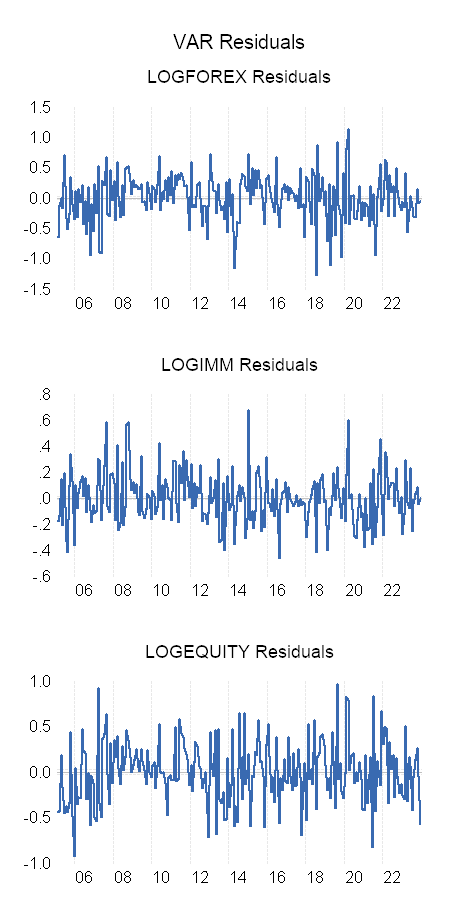
\includegraphics[scale=0.9]{annexes/msih_residuals.png}
    \label{fig:msih_resids}
\end{figure}

\begin{figure}[H]
    \centering
    \caption{Graphique des probabilités de transitions brutes du MSIH-VAR.}
    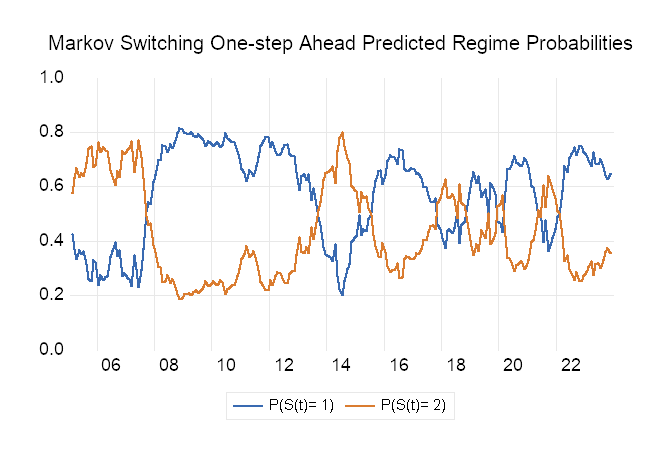
\includegraphics[scale=0.8]{annexes/msih_onestep.png}
    \label{fig:graph_prob_brutes}
\end{figure}

\begin{figure}[H]
    \centering
    \caption{Graphique des probabilités de transitions lisées du MSIH-VAR.}
    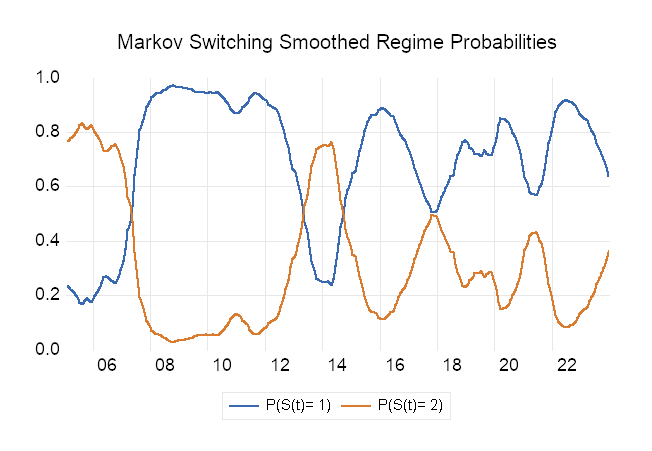
\includegraphics[scale=0.8]{annexes/msih_smoothed.png}
    \label{fig:graph_prob_lissees}
\end{figure}

\begin{table}[H]
    \centering
    \sffamily
    \caption{Test du portmanteau du modèle MISH-VAR.}
    \label{tab:test_portmanteau_var)}
    \resizebox{1\textwidth}{!}{\begin{tabular}{lrrrrr}
\multicolumn{6}{l}{VAR Residual Portmanteau Tests for Autocorrelations}\\
\multicolumn{6}{l}{Null Hypothesis: No residual autocorrelations up to lag h}\\
\multicolumn{3}{l}{Sample: 2005M01 2023M12}&\multicolumn{1}{c}{}&\multicolumn{1}{c}{}&\multicolumn{1}{c}{}\\
\multicolumn{3}{l}{Included observations: 227}&\multicolumn{1}{c}{}&\multicolumn{1}{c}{}&\multicolumn{1}{c}{}\\
[4.5pt] \hline \\ [-4.5pt]
\multicolumn{1}{c}{Lags}&\multicolumn{1}{c}{Q-Stat}&\multicolumn{1}{c}{Prob.*}&\multicolumn{1}{c}{Adj Q-Stat}&\multicolumn{1}{c}{Prob.*}&\multicolumn{1}{c}{df}\\
[4.5pt] \hline \\ [-4.5pt]
\multicolumn{1}{c}{1}&\multicolumn{1}{c}{$6.458256$}&\multicolumn{1}{c}{---}&\multicolumn{1}{c}{$6.486832$}&\multicolumn{1}{c}{---}&\multicolumn{1}{c}{---}\\
\multicolumn{1}{c}{2}&\multicolumn{1}{c}{$18.73100$}&\multicolumn{1}{c}{$0.0276$}&\multicolumn{1}{c}{$18.86867$}&\multicolumn{1}{c}{$0.0263$}&\multicolumn{1}{c}{9}\\
[4.5pt] \hline \\ [-4.5pt]
\multicolumn{6}{l}{*Test is valid only for lags larger than the VAR lag order.}\\
\multicolumn{7}{l}{df is degrees of freedom for (approximate) chi-square distribution}\\
\multicolumn{1}{c}{}&\multicolumn{1}{c}{}&\multicolumn{1}{c}{}&\multicolumn{1}{c}{}&\multicolumn{1}{c}{}&\multicolumn{1}{c}{}\\
\end{tabular}}
\end{table}

\begin{table}[H]
    \centering
    \sffamily
    \caption{Test de normalité du modèle MISH-VAR.}
    \label{tab:test_normalite_var}
    \resizebox{1\textwidth}{!}{\begin{tabular}{lrrrr}
\multicolumn{3}{l}{VAR Residual Normality Tests}&\multicolumn{1}{c}{}&\multicolumn{1}{c}{}\\
\multicolumn{4}{l}{Orthogonalization: Cholesky (Lutkepohl)}&\multicolumn{1}{c}{}\\
\multicolumn{5}{l}{Null Hypothesis: Residuals are multivariate normal}\\
\multicolumn{3}{l}{Sample: 2005M01 2023M12}&\multicolumn{1}{c}{}&\multicolumn{1}{c}{}\\
\multicolumn{3}{l}{Included observations: 227}&\multicolumn{1}{c}{}&\multicolumn{1}{c}{}\\
[4.5pt] \hline \\ [-4.5pt]
\multicolumn{1}{c}{}&\multicolumn{1}{c}{}&\multicolumn{1}{c}{}&\multicolumn{1}{c}{}&\multicolumn{1}{c}{}\\
\multicolumn{1}{c}{Component}&\multicolumn{1}{c}{Jarque-Bera}&\multicolumn{1}{c}{df}&\multicolumn{1}{c}{Prob.}&\multicolumn{1}{c}{}\\
[4.5pt] \hline \\ [-4.5pt]
\multicolumn{1}{c}{1}&\multicolumn{1}{c}{$5.760644$}&\multicolumn{1}{c}{2}&\multicolumn{1}{c}{$0.056117$}&\multicolumn{1}{c}{}\\
\multicolumn{1}{c}{2}&\multicolumn{1}{c}{$1.54375$}&\multicolumn{1}{c}{2}&\multicolumn{1}{c}{$0.4627$}&\multicolumn{1}{c}{}\\
\multicolumn{1}{c}{3}&\multicolumn{1}{c}{$4.746199$}&\multicolumn{1}{c}{2}&\multicolumn{1}{c}{$0.093191$}&\multicolumn{1}{c}{}\\
[4.5pt] \hline \\ [-4.5pt]
\multicolumn{1}{c}{Joint}&\multicolumn{1}{c}{$12.050593$}&\multicolumn{1}{c}{6}&\multicolumn{1}{c}{$0.049$}&\multicolumn{1}{c}{}\\
[4.5pt] \hline \\ [-4.5pt]
\multicolumn{6}{l}{*Approximate p-values do not account for coefficient}\\
\multicolumn{2}{l}{estimation}&\multicolumn{1}{c}{}&\multicolumn{1}{c}{}&\multicolumn{1}{c}{}\\
\multicolumn{1}{c}{}&\multicolumn{1}{c}{}&\multicolumn{1}{c}{}&\multicolumn{1}{c}{}&\multicolumn{1}{c}{}\\
\end{tabular}}
\end{table}

\subsubsection{Décomposition de la variance}

\begin{figure}[H]
    \centering
    \caption{Histogramme de décomposition de la variance du régime 1.}
    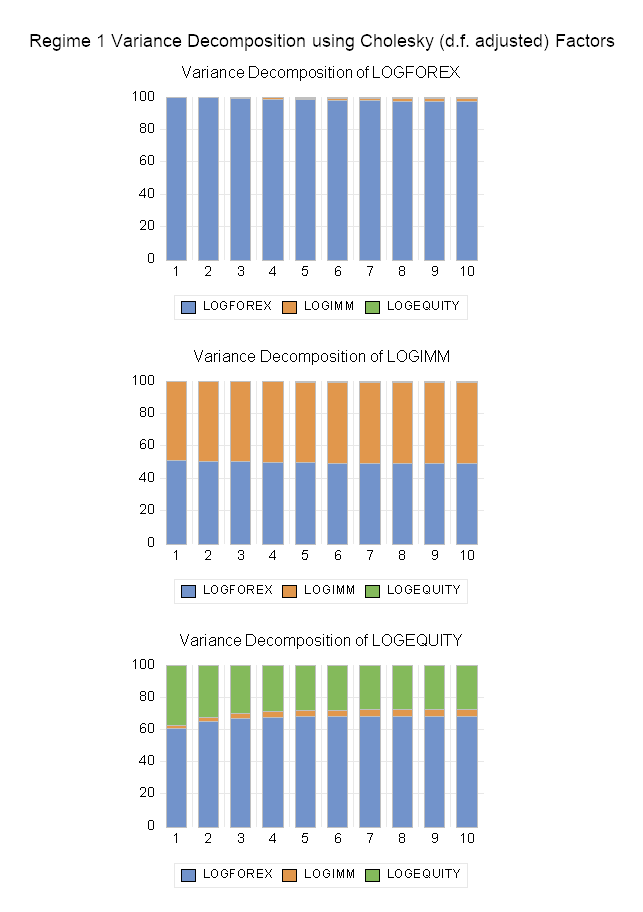
\includegraphics[scale=0.9]{annexes/regime_1.png}
    \label{fig:hist_variance_r1}
\end{figure}

\begin{figure}[H]
    \centering
    \caption{Histogramme de décomposition de la variance du régime 2.}
    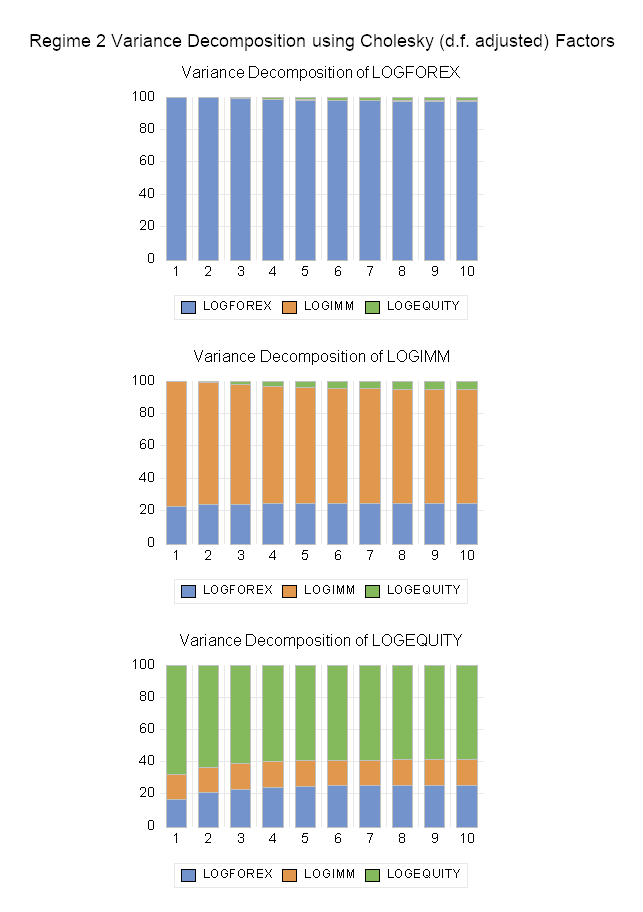
\includegraphics[scale=0.9]{annexes/regime_2.png}
    \label{fig:hist_variance_r2}
\end{figure}

\begin{table}[H]
    \centering
    \sffamily
    \caption{Tableau de décomposition de la variance du modèle 1.}
    \label{tab:tab_variance_r1}
    \resizebox{1\textwidth}{!}{\begin{tabular}{lrrrr}
\multicolumn{1}{c}{Variance Decomposition of LOGFOREX:}&\multicolumn{1}{c}{}&\multicolumn{1}{c}{}&\multicolumn{1}{c}{}&\multicolumn{1}{c}{}\\
\multicolumn{1}{l}{Period}&\multicolumn{1}{c}{S.E.}&\multicolumn{1}{c}{LOGFOREX}&\multicolumn{1}{c}{LOGIMM}&\multicolumn{1}{c}{LOGEQUITY}\\
[4.5pt] \hline \\ [-4.5pt]
\multicolumn{1}{c}{$1$}&\multicolumn{1}{c}{$0.304125$}&\multicolumn{1}{c}{$100.0000$}&\multicolumn{1}{c}{$0.000000$}&\multicolumn{1}{c}{$0.000000$}\\
\multicolumn{1}{c}{$2$}&\multicolumn{1}{c}{$0.364599$}&\multicolumn{1}{c}{$99.65702$}&\multicolumn{1}{c}{$0.139675$}&\multicolumn{1}{c}{$0.203303$}\\
\multicolumn{1}{c}{$3$}&\multicolumn{1}{c}{$0.389700$}&\multicolumn{1}{c}{$99.18205$}&\multicolumn{1}{c}{$0.407331$}&\multicolumn{1}{c}{$0.410614$}\\
\multicolumn{1}{c}{$4$}&\multicolumn{1}{c}{$0.401728$}&\multicolumn{1}{c}{$98.71024$}&\multicolumn{1}{c}{$0.733157$}&\multicolumn{1}{c}{$0.556603$}\\
\multicolumn{1}{c}{$5$}&\multicolumn{1}{c}{$0.408087$}&\multicolumn{1}{c}{$98.29265$}&\multicolumn{1}{c}{$1.060239$}&\multicolumn{1}{c}{$0.647109$}\\
\multicolumn{1}{c}{$6$}&\multicolumn{1}{c}{$0.411728$}&\multicolumn{1}{c}{$97.94471$}&\multicolumn{1}{c}{$1.354747$}&\multicolumn{1}{c}{$0.700546$}\\
\multicolumn{1}{c}{$7$}&\multicolumn{1}{c}{$0.413953$}&\multicolumn{1}{c}{$97.66572$}&\multicolumn{1}{c}{$1.602514$}&\multicolumn{1}{c}{$0.731762$}\\
\multicolumn{1}{c}{$8$}&\multicolumn{1}{c}{$0.415384$}&\multicolumn{1}{c}{$97.44793$}&\multicolumn{1}{c}{$1.801883$}&\multicolumn{1}{c}{$0.750185$}\\
\multicolumn{1}{c}{$9$}&\multicolumn{1}{c}{$0.416338$}&\multicolumn{1}{c}{$97.28114$}&\multicolumn{1}{c}{$1.957564$}&\multicolumn{1}{c}{$0.761296$}\\
\multicolumn{1}{c}{$10$}&\multicolumn{1}{c}{$0.416992$}&\multicolumn{1}{c}{$97.15517$}&\multicolumn{1}{c}{$2.076650$}&\multicolumn{1}{c}{$0.768178$}\\
[4.5pt] \hline \\ [-4.5pt]
\multicolumn{1}{c}{Variance Decomposition of LOGIMM:}&\multicolumn{1}{c}{}&\multicolumn{1}{c}{}&\multicolumn{1}{c}{}&\multicolumn{1}{c}{}\\
\multicolumn{1}{l}{Period}&\multicolumn{1}{c}{S.E.}&\multicolumn{1}{c}{LOGFOREX}&\multicolumn{1}{c}{LOGIMM}&\multicolumn{1}{c}{LOGEQUITY}\\
[4.5pt] \hline \\ [-4.5pt]
\multicolumn{1}{c}{$1$}&\multicolumn{1}{c}{$0.197859$}&\multicolumn{1}{c}{$51.14572$}&\multicolumn{1}{c}{$48.85428$}&\multicolumn{1}{c}{$0.000000$}\\
\multicolumn{1}{c}{$2$}&\multicolumn{1}{c}{$0.258028$}&\multicolumn{1}{c}{$50.52979$}&\multicolumn{1}{c}{$49.25963$}&\multicolumn{1}{c}{$0.210582$}\\
\multicolumn{1}{c}{$3$}&\multicolumn{1}{c}{$0.293564$}&\multicolumn{1}{c}{$50.04328$}&\multicolumn{1}{c}{$49.52211$}&\multicolumn{1}{c}{$0.434615$}\\
\multicolumn{1}{c}{$4$}&\multicolumn{1}{c}{$0.316703$}&\multicolumn{1}{c}{$49.68348$}&\multicolumn{1}{c}{$49.70874$}&\multicolumn{1}{c}{$0.607778$}\\
\multicolumn{1}{c}{$5$}&\multicolumn{1}{c}{$0.332438$}&\multicolumn{1}{c}{$49.42317$}&\multicolumn{1}{c}{$49.84636$}&\multicolumn{1}{c}{$0.730472$}\\
\multicolumn{1}{c}{$6$}&\multicolumn{1}{c}{$0.343393$}&\multicolumn{1}{c}{$49.23600$}&\multicolumn{1}{c}{$49.94878$}&\multicolumn{1}{c}{$0.815218$}\\
\multicolumn{1}{c}{$7$}&\multicolumn{1}{c}{$0.351132$}&\multicolumn{1}{c}{$49.10148$}&\multicolumn{1}{c}{$50.02494$}&\multicolumn{1}{c}{$0.873578$}\\
\multicolumn{1}{c}{$8$}&\multicolumn{1}{c}{$0.356650$}&\multicolumn{1}{c}{$49.00465$}&\multicolumn{1}{c}{$50.08136$}&\multicolumn{1}{c}{$0.913993$}\\
\multicolumn{1}{c}{$9$}&\multicolumn{1}{c}{$0.360608$}&\multicolumn{1}{c}{$48.93479$}&\multicolumn{1}{c}{$50.12299$}&\multicolumn{1}{c}{$0.942215$}\\
\multicolumn{1}{c}{$10$}&\multicolumn{1}{c}{$0.363460$}&\multicolumn{1}{c}{$48.88431$}&\multicolumn{1}{c}{$50.15360$}&\multicolumn{1}{c}{$0.962090$}\\
[4.5pt] \hline \\ [-4.5pt]
\multicolumn{1}{c}{Variance Decomposition of LOGEQUITY:}&\multicolumn{1}{c}{}&\multicolumn{1}{c}{}&\multicolumn{1}{c}{}&\multicolumn{1}{c}{}\\
\multicolumn{1}{l}{Period}&\multicolumn{1}{c}{S.E.}&\multicolumn{1}{c}{LOGFOREX}&\multicolumn{1}{c}{LOGIMM}&\multicolumn{1}{c}{LOGEQUITY}\\
[4.5pt] \hline \\ [-4.5pt]
\multicolumn{1}{c}{$1$}&\multicolumn{1}{c}{$0.218817$}&\multicolumn{1}{c}{$60.27540$}&\multicolumn{1}{c}{$2.020076$}&\multicolumn{1}{c}{$37.70453$}\\
\multicolumn{1}{c}{$2$}&\multicolumn{1}{c}{$0.251373$}&\multicolumn{1}{c}{$64.68915$}&\multicolumn{1}{c}{$2.496150$}&\multicolumn{1}{c}{$32.81470$}\\
\multicolumn{1}{c}{$3$}&\multicolumn{1}{c}{$0.263339$}&\multicolumn{1}{c}{$66.72249$}&\multicolumn{1}{c}{$2.951131$}&\multicolumn{1}{c}{$30.32638$}\\
\multicolumn{1}{c}{$4$}&\multicolumn{1}{c}{$0.268978$}&\multicolumn{1}{c}{$67.55629$}&\multicolumn{1}{c}{$3.360578$}&\multicolumn{1}{c}{$29.08313$}\\
\multicolumn{1}{c}{$5$}&\multicolumn{1}{c}{$0.272064$}&\multicolumn{1}{c}{$67.85628$}&\multicolumn{1}{c}{$3.711987$}&\multicolumn{1}{c}{$28.43173$}\\
\multicolumn{1}{c}{$6$}&\multicolumn{1}{c}{$0.273917$}&\multicolumn{1}{c}{$67.93461$}&\multicolumn{1}{c}{$4.001910$}&\multicolumn{1}{c}{$28.06347$}\\
\multicolumn{1}{c}{$7$}&\multicolumn{1}{c}{$0.275099$}&\multicolumn{1}{c}{$67.92733$}&\multicolumn{1}{c}{$4.233623$}&\multicolumn{1}{c}{$27.83905$}\\
\multicolumn{1}{c}{$8$}&\multicolumn{1}{c}{$0.275885$}&\multicolumn{1}{c}{$67.89177$}&\multicolumn{1}{c}{$4.414314$}&\multicolumn{1}{c}{$27.69391$}\\
\multicolumn{1}{c}{$9$}&\multicolumn{1}{c}{$0.276423$}&\multicolumn{1}{c}{$67.85126$}&\multicolumn{1}{c}{$4.552636$}&\multicolumn{1}{c}{$27.59610$}\\
\multicolumn{1}{c}{$10$}&\multicolumn{1}{c}{$0.276797$}&\multicolumn{1}{c}{$67.81454$}&\multicolumn{1}{c}{$4.657083$}&\multicolumn{1}{c}{$27.52837$}\\
[4.5pt] \hline \\ [-4.5pt]
\multicolumn{3}{l}{Cholesky One S.D. (d.f. adjusted)}&\multicolumn{1}{c}{}&\multicolumn{1}{c}{}\\
\multicolumn{5}{l}{Cholesky ordering:  LOGFOREX LOGIMM LOGEQUITY}\\
[4.5pt] \hline \\ [-4.5pt]
\end{tabular}}
\end{table}

\begin{table}[H]
    \centering
    \sffamily
    \caption{Tableau de décomposition de la variance du modèle 2.}
    \label{tab:tab_variance_r2}
    \resizebox{1\textwidth}{!}{\begin{tabular}{lrrrr}
\multicolumn{1}{c}{Variance Decomposition of LOGFOREX:}&\multicolumn{1}{c}{}&\multicolumn{1}{c}{}&\multicolumn{1}{c}{}&\multicolumn{1}{c}{}\\
\multicolumn{1}{l}{Period}&\multicolumn{1}{c}{S.E.}&\multicolumn{1}{c}{LOGFOREX}&\multicolumn{1}{c}{LOGIMM}&\multicolumn{1}{c}{LOGEQUITY}\\
[4.5pt] \hline \\ [-4.5pt]
\multicolumn{1}{c}{$1$}&\multicolumn{1}{c}{$0.415038$}&\multicolumn{1}{c}{$100.0000$}&\multicolumn{1}{c}{$0.000000$}&\multicolumn{1}{c}{$0.000000$}\\
\multicolumn{1}{c}{$2$}&\multicolumn{1}{c}{$0.496644$}&\multicolumn{1}{c}{$99.45607$}&\multicolumn{1}{c}{$0.005119$}&\multicolumn{1}{c}{$0.538808$}\\
\multicolumn{1}{c}{$3$}&\multicolumn{1}{c}{$0.528972$}&\multicolumn{1}{c}{$98.86155$}&\multicolumn{1}{c}{$0.042531$}&\multicolumn{1}{c}{$1.095918$}\\
\multicolumn{1}{c}{$4$}&\multicolumn{1}{c}{$0.543228$}&\multicolumn{1}{c}{$98.38060$}&\multicolumn{1}{c}{$0.122495$}&\multicolumn{1}{c}{$1.496909$}\\
\multicolumn{1}{c}{$5$}&\multicolumn{1}{c}{$0.549985$}&\multicolumn{1}{c}{$98.01558$}&\multicolumn{1}{c}{$0.232440$}&\multicolumn{1}{c}{$1.751985$}\\
\multicolumn{1}{c}{$6$}&\multicolumn{1}{c}{$0.553427$}&\multicolumn{1}{c}{$97.74044$}&\multicolumn{1}{c}{$0.352838$}&\multicolumn{1}{c}{$1.906723$}\\
\multicolumn{1}{c}{$7$}&\multicolumn{1}{c}{$0.555316$}&\multicolumn{1}{c}{$97.53238$}&\multicolumn{1}{c}{$0.468022$}&\multicolumn{1}{c}{$1.999598$}\\
\multicolumn{1}{c}{$8$}&\multicolumn{1}{c}{$0.556430$}&\multicolumn{1}{c}{$97.37499$}&\multicolumn{1}{c}{$0.569136$}&\multicolumn{1}{c}{$2.055876$}\\
\multicolumn{1}{c}{$9$}&\multicolumn{1}{c}{$0.557128$}&\multicolumn{1}{c}{$97.25634$}&\multicolumn{1}{c}{$0.652985$}&\multicolumn{1}{c}{$2.090672$}\\
\multicolumn{1}{c}{$10$}&\multicolumn{1}{c}{$0.557587$}&\multicolumn{1}{c}{$97.16740$}&\multicolumn{1}{c}{$0.719881$}&\multicolumn{1}{c}{$2.112723$}\\
[4.5pt] \hline \\ [-4.5pt]
\multicolumn{1}{c}{Variance Decomposition of LOGIMM:}&\multicolumn{1}{c}{}&\multicolumn{1}{c}{}&\multicolumn{1}{c}{}&\multicolumn{1}{c}{}\\
\multicolumn{1}{l}{Period}&\multicolumn{1}{c}{S.E.}&\multicolumn{1}{c}{LOGFOREX}&\multicolumn{1}{c}{LOGIMM}&\multicolumn{1}{c}{LOGEQUITY}\\
[4.5pt] \hline \\ [-4.5pt]
\multicolumn{1}{c}{$1$}&\multicolumn{1}{c}{$0.188015$}&\multicolumn{1}{c}{$22.60091$}&\multicolumn{1}{c}{$77.39909$}&\multicolumn{1}{c}{$0.000000$}\\
\multicolumn{1}{c}{$2$}&\multicolumn{1}{c}{$0.243005$}&\multicolumn{1}{c}{$23.58616$}&\multicolumn{1}{c}{$75.24629$}&\multicolumn{1}{c}{$1.167544$}\\
\multicolumn{1}{c}{$3$}&\multicolumn{1}{c}{$0.275579$}&\multicolumn{1}{c}{$23.98151$}&\multicolumn{1}{c}{$73.59318$}&\multicolumn{1}{c}{$2.425316$}\\
\multicolumn{1}{c}{$4$}&\multicolumn{1}{c}{$0.296923$}&\multicolumn{1}{c}{$24.12792$}&\multicolumn{1}{c}{$72.47180$}&\multicolumn{1}{c}{$3.400274$}\\
\multicolumn{1}{c}{$5$}&\multicolumn{1}{c}{$0.311498$}&\multicolumn{1}{c}{$24.17106$}&\multicolumn{1}{c}{$71.73760$}&\multicolumn{1}{c}{$4.091338$}\\
\multicolumn{1}{c}{$6$}&\multicolumn{1}{c}{$0.321669$}&\multicolumn{1}{c}{$24.17293$}&\multicolumn{1}{c}{$71.25840$}&\multicolumn{1}{c}{$4.568664$}\\
\multicolumn{1}{c}{$7$}&\multicolumn{1}{c}{$0.328862$}&\multicolumn{1}{c}{$24.16008$}&\multicolumn{1}{c}{$70.94251$}&\multicolumn{1}{c}{$4.897402$}\\
\multicolumn{1}{c}{$8$}&\multicolumn{1}{c}{$0.333993$}&\multicolumn{1}{c}{$24.14372$}&\multicolumn{1}{c}{$70.73118$}&\multicolumn{1}{c}{$5.125106$}\\
\multicolumn{1}{c}{$9$}&\multicolumn{1}{c}{$0.337674$}&\multicolumn{1}{c}{$24.12827$}&\multicolumn{1}{c}{$70.58757$}&\multicolumn{1}{c}{$5.284153$}\\
\multicolumn{1}{c}{$10$}&\multicolumn{1}{c}{$0.340327$}&\multicolumn{1}{c}{$24.11524$}&\multicolumn{1}{c}{$70.48858$}&\multicolumn{1}{c}{$5.396184$}\\
[4.5pt] \hline \\ [-4.5pt]
\multicolumn{1}{c}{Variance Decomposition of LOGEQUITY:}&\multicolumn{1}{c}{}&\multicolumn{1}{c}{}&\multicolumn{1}{c}{}&\multicolumn{1}{c}{}\\
\multicolumn{1}{l}{Period}&\multicolumn{1}{c}{S.E.}&\multicolumn{1}{c}{LOGFOREX}&\multicolumn{1}{c}{LOGIMM}&\multicolumn{1}{c}{LOGEQUITY}\\
[4.5pt] \hline \\ [-4.5pt]
\multicolumn{1}{c}{$1$}&\multicolumn{1}{c}{$0.360736$}&\multicolumn{1}{c}{$16.42181$}&\multicolumn{1}{c}{$15.35604$}&\multicolumn{1}{c}{$68.22215$}\\
\multicolumn{1}{c}{$2$}&\multicolumn{1}{c}{$0.399543$}&\multicolumn{1}{c}{$20.56477$}&\multicolumn{1}{c}{$15.56026$}&\multicolumn{1}{c}{$63.87498$}\\
\multicolumn{1}{c}{$3$}&\multicolumn{1}{c}{$0.410371$}&\multicolumn{1}{c}{$22.92458$}&\multicolumn{1}{c}{$15.66404$}&\multicolumn{1}{c}{$61.41138$}\\
\multicolumn{1}{c}{$4$}&\multicolumn{1}{c}{$0.414715$}&\multicolumn{1}{c}{$24.10645$}&\multicolumn{1}{c}{$15.73111$}&\multicolumn{1}{c}{$60.16245$}\\
\multicolumn{1}{c}{$5$}&\multicolumn{1}{c}{$0.416914$}&\multicolumn{1}{c}{$24.66861$}&\multicolumn{1}{c}{$15.79222$}&\multicolumn{1}{c}{$59.53917$}\\
\multicolumn{1}{c}{$6$}&\multicolumn{1}{c}{$0.418169$}&\multicolumn{1}{c}{$24.93277$}&\multicolumn{1}{c}{$15.85304$}&\multicolumn{1}{c}{$59.21420$}\\
\multicolumn{1}{c}{$7$}&\multicolumn{1}{c}{$0.418937$}&\multicolumn{1}{c}{$25.05740$}&\multicolumn{1}{c}{$15.91065$}&\multicolumn{1}{c}{$59.03195$}\\
\multicolumn{1}{c}{$8$}&\multicolumn{1}{c}{$0.419429$}&\multicolumn{1}{c}{$25.11669$}&\multicolumn{1}{c}{$15.96169$}&\multicolumn{1}{c}{$58.92162$}\\
\multicolumn{1}{c}{$9$}&\multicolumn{1}{c}{$0.419757$}&\multicolumn{1}{c}{$25.14505$}&\multicolumn{1}{c}{$16.00450$}&\multicolumn{1}{c}{$58.85045$}\\
\multicolumn{1}{c}{$10$}&\multicolumn{1}{c}{$0.419981$}&\multicolumn{1}{c}{$25.15861$}&\multicolumn{1}{c}{$16.03900$}&\multicolumn{1}{c}{$58.80239$}\\
[4.5pt] \hline \\ [-4.5pt]
\multicolumn{3}{l}{Cholesky One S.D. (d.f. adjusted)}&\multicolumn{1}{c}{}&\multicolumn{1}{c}{}\\
\multicolumn{5}{l}{Cholesky ordering:  LOGFOREX LOGIMM LOGEQUITY}\\
[4.5pt] \hline \\ [-4.5pt]
\end{tabular}}
\end{table}

\begin{figure}[H]
    \centering
    \caption{Décomposition historique du régime 2.}
    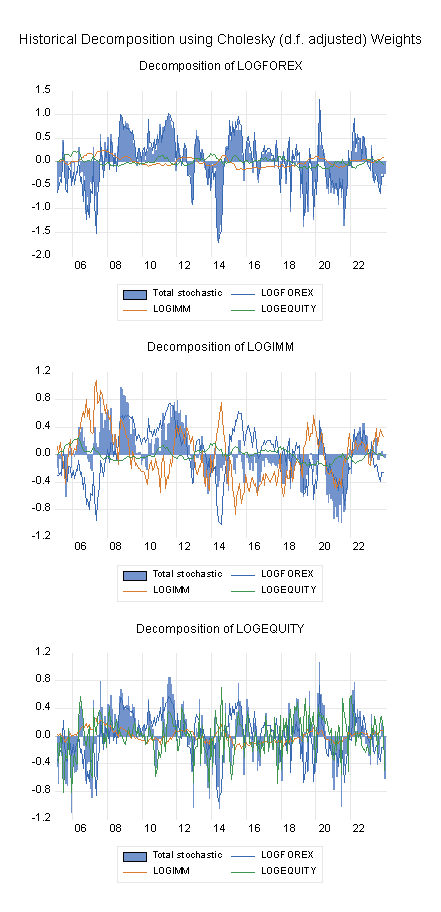
\includegraphics[scale=1]{annexes/regime_1_historcal_decomposition.png}
    \label{fig:msih_resids}
\end{figure}

\begin{figure}[H]
    \centering
    \caption{Décomposition historique du régime 2.}
    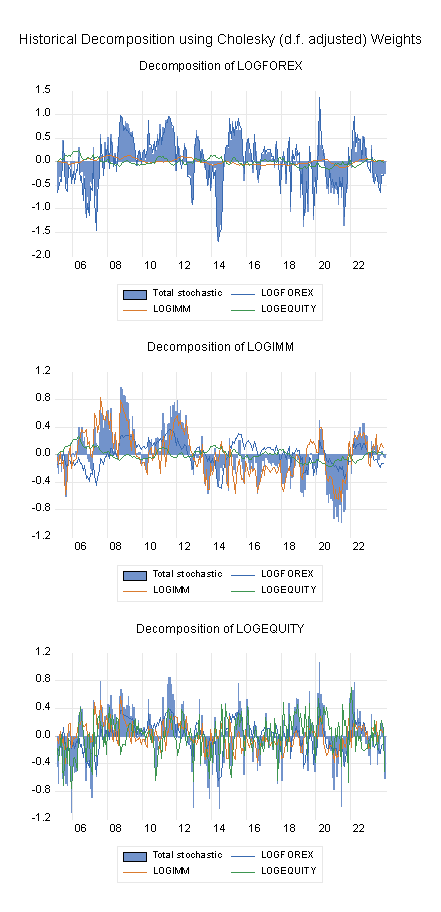
\includegraphics[scale=1]{annexes/regime_2_historical_decomposition.png}
    \label{fig:msih_resids}
\end{figure}

\subsubsection{Fonctions de réponses impulsionnelles}

\begin{figure}[H]
    \centering
    \caption{Réponses impulsionnelles du régime 1.}
    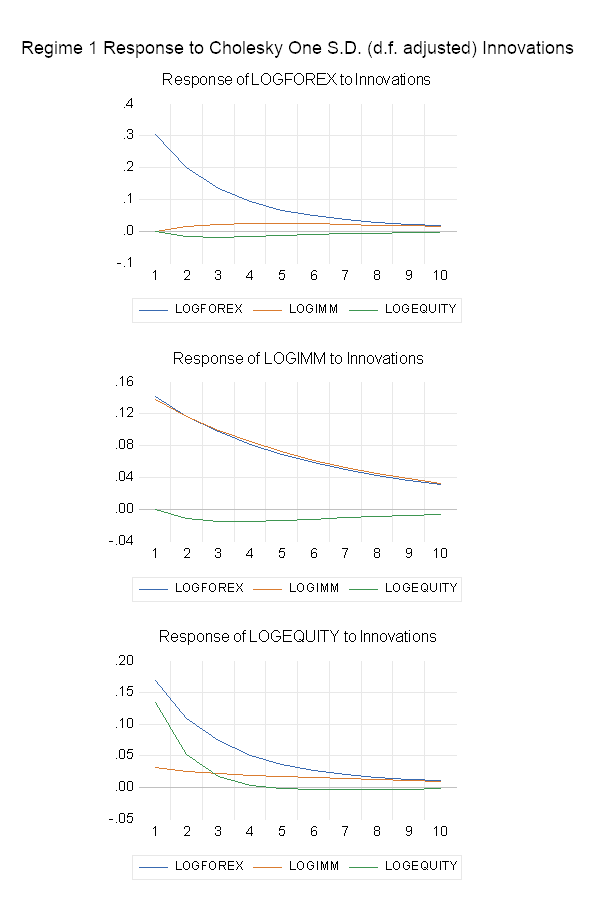
\includegraphics[scale=0.9]{annexes/regime_1_implusereponse.png}
    \label{fig:impulse_reponse_r1}
\end{figure}

\begin{figure}[H]
    \centering
    \caption{Réponses impulsionnelles du régime 2.}
    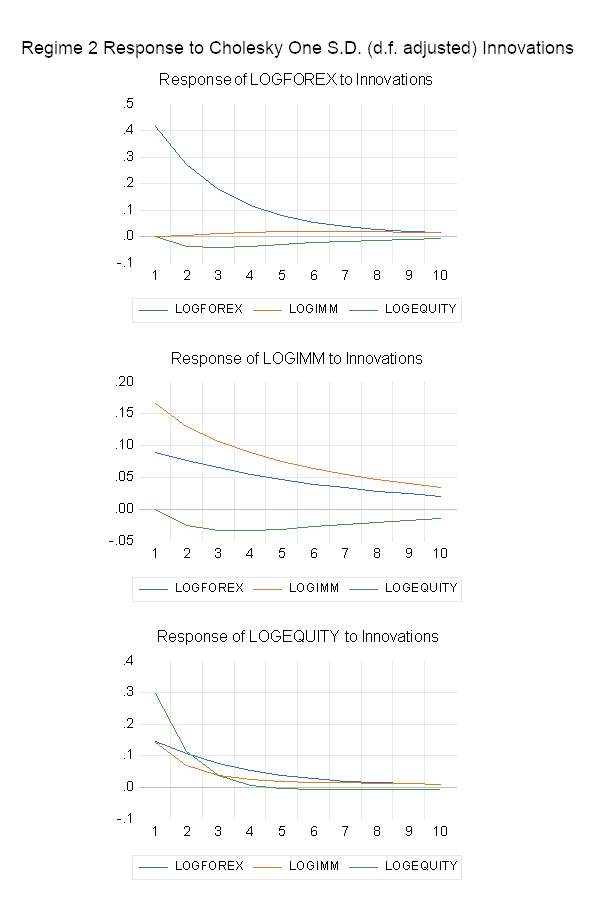
\includegraphics[scale=1]{annexes/regime_2_impulsereponse.png}
    \label{fig:impulse_reponse_r2}
\end{figure}

\begin{figure}[H]
    \centering
    \caption{Réponse impulsionnelle détaillées du régime 1.}
    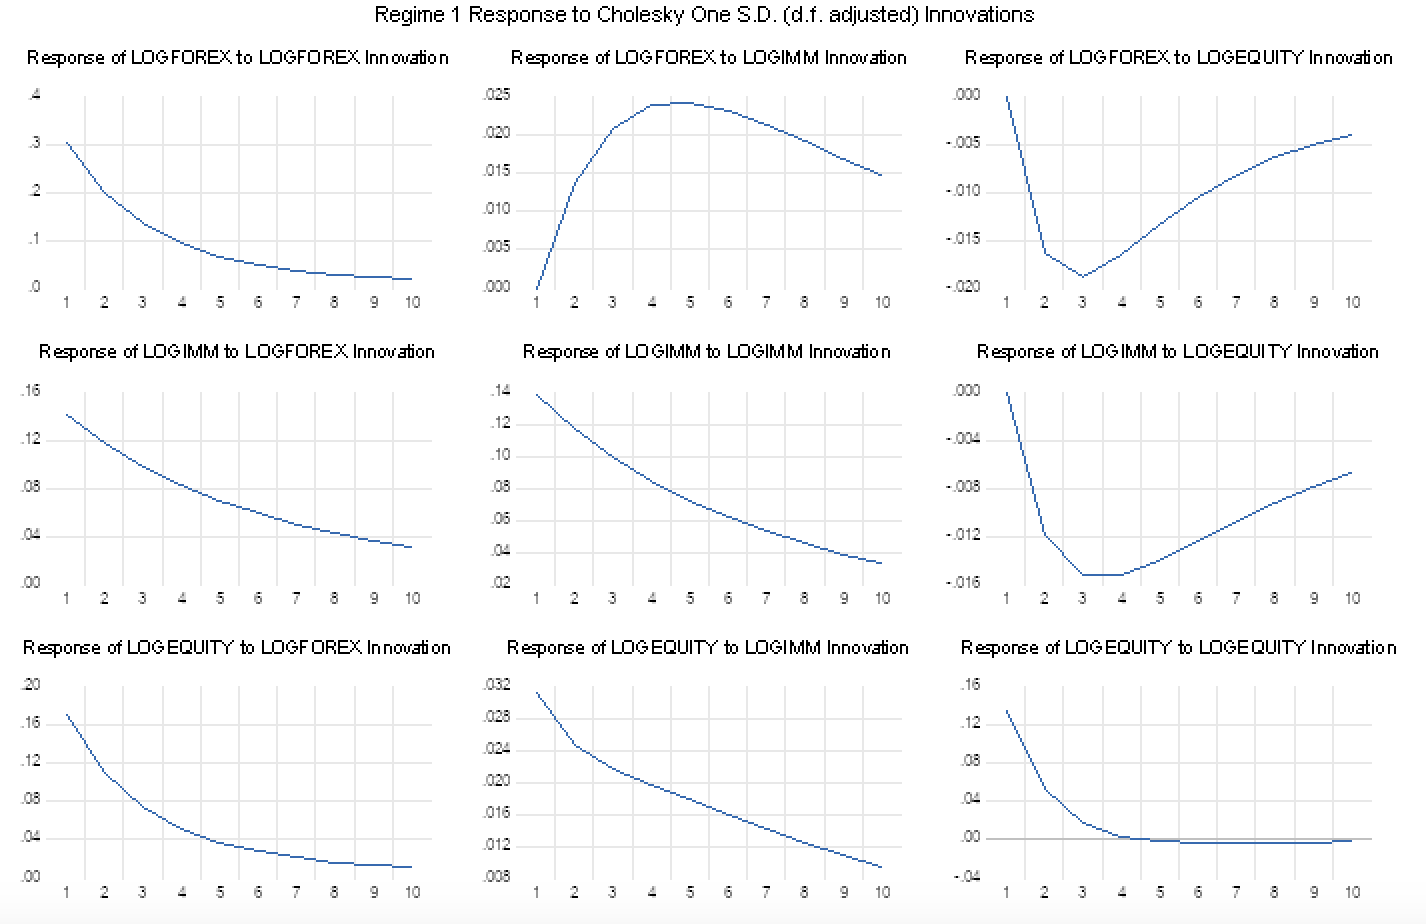
\includegraphics[scale=0.65]{annexes/regime1_mutiple_reponses.png}
    \label{fig:msih_resids}
\end{figure}

\begin{figure}[H]
    \centering
    \caption{Réponse impulsionnelle détaillées du régime 2.}
    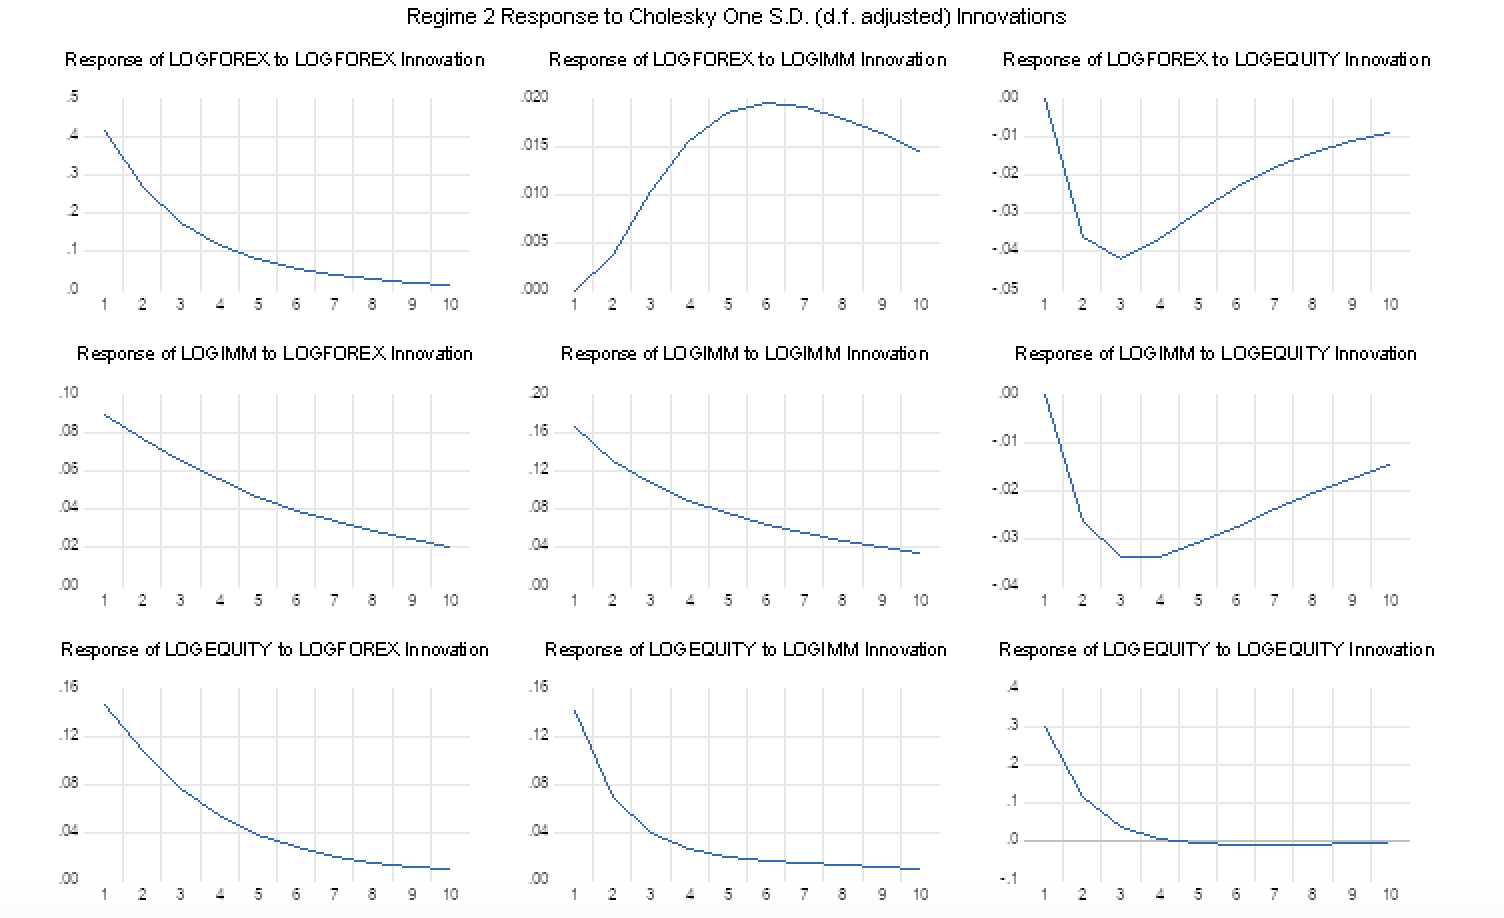
\includegraphics[scale=0.65]{annexes/regime2_multiples_reponses.png}
    \label{fig:msih_resids}
\end{figure}

\subsection{Estimation du modèle NARDL}

\subsubsection{Estimation du modèle NARDL sur le marché interbancaire}

\begin{table}[H]
    \centering
    \sffamily
    \caption{Estimation du modèle NARDL sur le LOGIMM.}
    \label{tab:nardl_logimm}
    \resizebox{1\textwidth}{!}{\begin{tabular}{lrrrr}
\multicolumn{2}{l}{Dependent Variable: LOGIMM}&\multicolumn{1}{c}{}&\multicolumn{1}{c}{}&\multicolumn{1}{c}{}\\
\multicolumn{1}{l}{Method: ARDL}&\multicolumn{1}{c}{}&\multicolumn{1}{c}{}&\multicolumn{1}{c}{}&\multicolumn{1}{c}{}\\
\multicolumn{3}{l}{Sample (adjusted): 2005M04 2023M12}&\multicolumn{1}{c}{}&\multicolumn{1}{c}{}\\
\multicolumn{4}{l}{Included observations: 225 after adjustments}&\multicolumn{1}{c}{}\\
\multicolumn{4}{l}{Maximum dependent lags: 4 (Automatic selection)}&\multicolumn{1}{c}{}\\
\multicolumn{4}{l}{Model selection method: Akaike info criterion (AIC)}&\multicolumn{1}{c}{}\\
\multicolumn{5}{l}{Dynamic regressors : LOGFOREX\_POS}\\
\multicolumn{5}{l}{LOGFOREX\_NEG  LOGEQUITY\_POS LOGEQUITY\_NEG}\\
\multicolumn{1}{l}{Fixed regressors: C}&\multicolumn{1}{c}{}&\multicolumn{1}{c}{}&\multicolumn{1}{c}{}&\multicolumn{1}{c}{}\\
\multicolumn{3}{l}{Number of models evaluated: 2500}&\multicolumn{1}{c}{}&\multicolumn{1}{c}{}\\
\multicolumn{3}{l}{Selected Model: ARDL(3, 1, 0, 1, 1)}&\multicolumn{1}{c}{}&\multicolumn{1}{c}{}\\
\multicolumn{6}{l}{HAC standard errors \& covariance} \\{}&\multicolumn{1}{c}{}&\multicolumn{1}{c}{} \\
[4.5pt] \hline \\ [-4.5pt]
\multicolumn{1}{c}{Variable}&\multicolumn{1}{r}{Coefficient}&\multicolumn{1}{r}{Std. Error}&\multicolumn{1}{r}{t-Statistic}&\multicolumn{1}{r}{Prob.*}\\
[4.5pt] \hline \\ [-4.5pt]
\multicolumn{1}{c}{LOGIMM(-1)}&\multicolumn{1}{r}{$0.838641$}&\multicolumn{1}{r}{$0.059959$}&\multicolumn{1}{r}{$13.98694$}&\multicolumn{1}{r}{$0.0000$}\\
\multicolumn{1}{c}{LOGIMM(-2)}&\multicolumn{1}{r}{$-0.161290$}&\multicolumn{1}{r}{$0.064646$}&\multicolumn{1}{r}{$-2.494978$}&\multicolumn{1}{r}{$0.0134$}\\
\multicolumn{1}{c}{LOGIMM(-3)}&\multicolumn{1}{r}{$0.097142$}&\multicolumn{1}{r}{$0.039186$}&\multicolumn{1}{r}{$2.479022$}&\multicolumn{1}{r}{$0.0139$}\\
\multicolumn{1}{c}{LOGFOREX\_POS}&\multicolumn{1}{r}{$0.313457$}&\multicolumn{1}{r}{$0.052513$}&\multicolumn{1}{r}{$5.969120$}&\multicolumn{1}{r}{$0.0000$}\\
\multicolumn{1}{c}{LOGFOREX\_POS(-1)}&\multicolumn{1}{r}{$-0.216963$}&\multicolumn{1}{r}{$0.046805$}&\multicolumn{1}{r}{$-4.635433$}&\multicolumn{1}{r}{$0.0000$}\\
\multicolumn{1}{c}{LOGFOREX\_NEG}&\multicolumn{1}{r}{$0.072413$}&\multicolumn{1}{r}{$0.024569$}&\multicolumn{1}{r}{$2.947298$}&\multicolumn{1}{r}{$0.0036$}\\
\multicolumn{1}{c}{LOGEQUITY\_POS}&\multicolumn{1}{r}{$0.190579$}&\multicolumn{1}{r}{$0.051848$}&\multicolumn{1}{r}{$3.675710$}&\multicolumn{1}{r}{$0.0003$}\\
\multicolumn{1}{c}{LOGEQUITY\_POS(-1)}&\multicolumn{1}{r}{$-0.127202$}&\multicolumn{1}{r}{$0.044382$}&\multicolumn{1}{r}{$-2.866090$}&\multicolumn{1}{r}{$0.0046$}\\
\multicolumn{1}{c}{LOGEQUITY\_NEG}&\multicolumn{1}{r}{$0.277842$}&\multicolumn{1}{r}{$0.056744$}&\multicolumn{1}{r}{$4.896384$}&\multicolumn{1}{r}{$0.0000$}\\
\multicolumn{1}{c}{LOGEQUITY\_NEG(-1)}&\multicolumn{1}{r}{$-0.185179$}&\multicolumn{1}{r}{$0.067938$}&\multicolumn{1}{r}{$-2.725690$}&\multicolumn{1}{r}{$0.0069$}\\
\multicolumn{1}{c}{C}&\multicolumn{1}{r}{$0.163384$}&\multicolumn{1}{r}{$0.058793$}&\multicolumn{1}{r}{$2.778979$}&\multicolumn{1}{r}{$0.0059$}\\
[4.5pt] \hline \\ [-4.5pt]
\multicolumn{1}{l}{R-squared}&\multicolumn{1}{r}{$0.916264$}&\multicolumn{2}{l}{Mean dependent var}&\multicolumn{1}{r}{$1.363154$}\\
\multicolumn{1}{l}{Adjusted R-squared}&\multicolumn{1}{r}{$0.912351$}&\multicolumn{2}{l}{S.D. dependent var}&\multicolumn{1}{r}{$0.491108$}\\
\multicolumn{1}{l}{S.E. of regression}&\multicolumn{1}{r}{$0.145395$}&\multicolumn{2}{l}{Akaike info criterion}&\multicolumn{1}{r}{$-0.971070$}\\
\multicolumn{1}{l}{Sum squared resid}&\multicolumn{1}{r}{$4.523904$}&\multicolumn{2}{l}{Schwarz criterion}&\multicolumn{1}{r}{$-0.804061$}\\
\multicolumn{1}{l}{Log likelihood}&\multicolumn{1}{r}{$120.2454$}&\multicolumn{2}{l}{Hannan-Quinn criter.}&\multicolumn{1}{r}{$-0.903665$}\\
\multicolumn{1}{l}{F-statistic}&\multicolumn{1}{r}{$234.1656$}&\multicolumn{2}{l}{Durbin-Watson stat}&\multicolumn{1}{r}{$2.019332$}\\
\multicolumn{1}{l}{Prob(F-statistic)}&\multicolumn{1}{r}{$0.000000$}&\multicolumn{1}{c}{}&\multicolumn{1}{c}{}&\multicolumn{1}{c}{}\\
[4.5pt] \hline \\ [-4.5pt]
\multicolumn{1}{l}{selection.}&\multicolumn{1}{c}{}&\multicolumn{1}{c}{}&\multicolumn{1}{c}{}&\multicolumn{1}{c}{}\\
\end{tabular}
}
\end{table}

\begin{table}[H]
    \centering
    \sffamily
    \caption{Test d'existence des asymétries sur le modèle NARDL LOGIMM.}
    \label{tab:asymetrie_nardl_logimm}
    \resizebox{0.8\textwidth}{!}{\begin{tabular}{lrrr}
\multicolumn{1}{l}{Wald Test:}&\multicolumn{1}{c}{}&\multicolumn{1}{c}{}&\multicolumn{1}{c}{}\\
\multicolumn{2}{l}{Equation: NARDL03}&\multicolumn{1}{c}{}&\multicolumn{1}{c}{}\\
[4.5pt] \hline \\ [-4.5pt]
\multicolumn{1}{l}{Test Statistic}&\multicolumn{1}{c}{Value}&\multicolumn{1}{c}{df}&\multicolumn{1}{c}{Probability}\\
[4.5pt] \hline \\ [-4.5pt]
\multicolumn{1}{l}{F-statistic}&\multicolumn{1}{c}{$8.856966$}&\multicolumn{1}{c}{(4, 214)}&\multicolumn{1}{c}{$0.0000$}\\
\multicolumn{1}{l}{Chi-square}&\multicolumn{1}{c}{$35.42787$}&\multicolumn{1}{c}{$4$}&\multicolumn{1}{c}{$0.0000$}\\
[4.5pt] \hline \\ [-4.5pt]
\multicolumn{1}{c}{}&\multicolumn{1}{c}{}&\multicolumn{1}{c}{}&\multicolumn{1}{c}{}\\
\multicolumn{5}{l}{Null Hypothesis: C(4) = C(6), C(5) = 0,}\\
\multicolumn{1}{l}{C(7) = C(9), C(8) =C(10)}&\multicolumn{1}{c}{}&\multicolumn{1}{c}{}&\multicolumn{1}{c}{}\\
\multicolumn{2}{l}{Null Hypothesis Summary:}&\multicolumn{1}{c}{}&\multicolumn{1}{c}{}\\
[4.5pt] \hline \\ [-4.5pt]
\multicolumn{2}{l}{Normalized Restriction (= 0)}&\multicolumn{1}{c}{Value}&\multicolumn{1}{c}{Std. Err.}\\
[4.5pt] \hline \\ [-4.5pt]
\multicolumn{1}{l}{C(4) - C(6)}&\multicolumn{1}{c}{}&\multicolumn{1}{c}{$0.241045$}&\multicolumn{1}{c}{$0.047354$}\\
\multicolumn{1}{l}{C(5)}&\multicolumn{1}{c}{}&\multicolumn{1}{c}{$-0.216963$}&\multicolumn{1}{c}{$0.046805$}\\
\multicolumn{1}{l}{C(7) - C(9)}&\multicolumn{1}{c}{}&\multicolumn{1}{c}{$-0.087263$}&\multicolumn{1}{c}{$0.090034$}\\
\multicolumn{1}{l}{C(8) - C(10)}&\multicolumn{1}{c}{}&\multicolumn{1}{c}{$0.057977$}&\multicolumn{1}{c}{$0.083753$}\\
[4.5pt] \hline \\ [-4.5pt]
\multicolumn{3}{l}{Restrictions are linear in coefficients.}&\multicolumn{1}{c}{}\\
\end{tabular}}
\end{table}

\begin{table}[H]
    \centering
    \sffamily
    \caption{Test de multicolinéarité (VIF) sur le modèle NARDL LOGIMM.}
    \label{tab:vif_nardl_logimm}
    \resizebox{0.8\textwidth}{!}{\begin{tabular}{lrrr}
\multicolumn{2}{l}{Variance Inflation Factors}&\multicolumn{1}{c}{}&\multicolumn{1}{c}{}\\
\multicolumn{2}{l}{Sample: 2005M01 2023M12}&\multicolumn{1}{c}{}&\multicolumn{1}{c}{}\\
\multicolumn{2}{l}{Included observations: 225}&\multicolumn{1}{c}{}&\multicolumn{1}{c}{}\\
[4.5pt] \hline \\ [-4.5pt]
\multicolumn{1}{c}{}&\multicolumn{1}{c}{Coefficient}&\multicolumn{1}{c}{Uncentered}&\multicolumn{1}{c}{Centered}\\
\multicolumn{1}{c}{Variable}&\multicolumn{1}{c}{Variance}&\multicolumn{1}{c}{VIF}&\multicolumn{1}{c}{VIF}\\
[4.5pt] \hline \\ [-4.5pt]
\multicolumn{1}{c}{LOGIMM(-1)}&\multicolumn{1}{c}{$0.003595$}&\multicolumn{1}{c}{$88.95157$}&\multicolumn{1}{c}{$11.45420$}\\
\multicolumn{1}{c}{LOGIMM(-2)}&\multicolumn{1}{c}{$0.004179$}&\multicolumn{1}{c}{$109.1952$}&\multicolumn{1}{c}{$15.65318$}\\
\multicolumn{1}{c}{LOGIMM(-3)}&\multicolumn{1}{c}{$0.001536$}&\multicolumn{1}{c}{$40.86455$}&\multicolumn{1}{c}{$6.780867$}\\
\multicolumn{1}{c}{LOGFOREX\_POS}&\multicolumn{1}{c}{$0.002758$}&\multicolumn{1}{c}{$15347.74$}&\multicolumn{1}{c}{$3607.471$}\\
\multicolumn{1}{c}{LOGFOREX\_POS(-1)}&\multicolumn{1}{c}{$0.002191$}&\multicolumn{1}{c}{$11972.51$}&\multicolumn{1}{c}{$2871.852$}\\
\multicolumn{1}{c}{LOGFOREX\_NEG}&\multicolumn{1}{c}{$0.000604$}&\multicolumn{1}{c}{$3249.708$}&\multicolumn{1}{c}{$807.2229$}\\
\multicolumn{1}{c}{LOGEQUITY\_POS}&\multicolumn{1}{c}{$0.002688$}&\multicolumn{1}{c}{$13237.66$}&\multicolumn{1}{c}{$3119.525$}\\
\multicolumn{1}{c}{LOGEQUITY\_POS(-1)}&\multicolumn{1}{c}{$0.001970$}&\multicolumn{1}{c}{$9509.601$}&\multicolumn{1}{c}{$2272.356$}\\
\multicolumn{1}{c}{LOGEQUITY\_NEG}&\multicolumn{1}{c}{$0.003220$}&\multicolumn{1}{c}{$13849.75$}&\multicolumn{1}{c}{$3687.246$}\\
\multicolumn{1}{c}{LOGEQUITY\_NEG(-1)}&\multicolumn{1}{c}{$0.004616$}&\multicolumn{1}{c}{$19669.81$}&\multicolumn{1}{c}{$5329.415$}\\
\multicolumn{1}{c}{C}&\multicolumn{1}{c}{$0.003457$}&\multicolumn{1}{c}{$47.52094$}&\multicolumn{1}{c}{$NA$}\\
[4.5pt] \hline \\ [-4.5pt]
\end{tabular}}
\end{table}

\begin{table}[H]
    \centering
    \sffamily
    \caption{Test de redondance des variables asymétriques dans le modèle NARDL LOGIMM.}
    \label{tab:redondance_nardl_logimm}
    \resizebox{1\textwidth}{!}{\begin{tabular}{lrrrr}
\multicolumn{2}{l}{Redundant Variables Test}&\multicolumn{1}{c}{}&\multicolumn{1}{c}{}&\multicolumn{1}{c}{}\\
\multicolumn{1}{l}{Equation: NARDL03}&\multicolumn{1}{c}{}&\multicolumn{1}{c}{}&\multicolumn{1}{c}{}&\multicolumn{1}{c}{}\\
\multicolumn{5}{l}{Redundant variables: LOGFOREX\_NEG LOGFOREX\_POS}\\
\multicolumn{5}{l}{LOGEQUITY\_POS LOGEQUITY\_NEG LOGFOREX\_POS(-1)}\\
\multicolumn{4}{l}{LOGEQUITY\_POS(-1) LOGEQUITY\_NEG(-1)}&\multicolumn{1}{c}{}\\
\multicolumn{5}{l}{Specification: LOGIMM LOGIMM(-1) LOGIMM(-2) LOGIMM(-3)}\\
\multicolumn{5}{l}{LOGFOREX\_POS LOGFOREX\_POS(-1) LOGFOREX\_NEG}\\
\multicolumn{5}{l}{LOGEQUITY\_POS LOGEQUITY\_POS(-1) LOGEQUITY\_NEG}\\
\multicolumn{2}{l}{LOGEQUITY\_NEG(-1) C}&\multicolumn{1}{c}{}&\multicolumn{1}{c}{}&\multicolumn{1}{c}{}\\
\multicolumn{6}{l}{Null hypothesis: LOGFOREX\_NEG LOGFOREX\_POS LOGEQUITY\_POS}\\
\multicolumn{6}{l}{LOGEQUITY\_NEG LOGFOREX\_POS(-1) LOGEQUITY\_POS(-1)}\\
\multicolumn{4}{l}{LOGEQUITY\_NEG(-1) are jointly insignificant}&\multicolumn{1}{c}{}\\
[4.5pt] \hline \\ [-4.5pt]
\multicolumn{1}{c}{}&\multicolumn{1}{c}{Value}&\multicolumn{1}{c}{df}&\multicolumn{1}{c}{Probability}&\multicolumn{1}{c}{}\\
\multicolumn{1}{l}{F-statistic}&\multicolumn{1}{c}{$29.94530$}&\multicolumn{1}{c}{(7, 214)}&\multicolumn{1}{c}{$0.0000$}&\multicolumn{1}{c}{}\\
[4.5pt] \hline \\ [-4.5pt]
\multicolumn{1}{l}{F-test summary:}&\multicolumn{1}{c}{}&\multicolumn{1}{c}{}&\multicolumn{1}{c}{}&\multicolumn{1}{c}{}\\
\multicolumn{1}{c}{}&\multicolumn{1}{c}{Sum of Sq.}&\multicolumn{1}{c}{df}&\multicolumn{1}{c}{Mean Squares}&\multicolumn{1}{c}{}\\
\multicolumn{1}{l}{Test SSR}&\multicolumn{1}{c}{$4.431250$}&\multicolumn{1}{c}{$7$}&\multicolumn{1}{c}{$0.633036$}&\multicolumn{1}{c}{}\\
\multicolumn{1}{l}{Restricted SSR}&\multicolumn{1}{c}{$8.955154$}&\multicolumn{1}{c}{$221$}&\multicolumn{1}{c}{$0.040521$}&\multicolumn{1}{c}{}\\
\multicolumn{1}{l}{Unrestricted SSR}&\multicolumn{1}{c}{$4.523904$}&\multicolumn{1}{c}{$214$}&\multicolumn{1}{c}{$0.021140$}&\multicolumn{1}{c}{}\\
[4.5pt] \hline \\ [-4.5pt]
\multicolumn{1}{c}{}&\multicolumn{1}{c}{}&\multicolumn{1}{c}{}&\multicolumn{1}{c}{}&\multicolumn{1}{c}{}\\
\multicolumn{2}{l}{Restricted Test Equation:}&\multicolumn{1}{c}{}&\multicolumn{1}{c}{}&\multicolumn{1}{c}{}\\
\multicolumn{2}{l}{Dependent Variable: LOGIMM}&\multicolumn{1}{c}{}&\multicolumn{1}{c}{}&\multicolumn{1}{c}{}\\
\multicolumn{2}{l}{Method: Least Squares}&\multicolumn{1}{c}{}&\multicolumn{1}{c}{}&\multicolumn{1}{c}{}\\
\multicolumn{2}{l}{Date: 11/12/24   Time: 22:07}&\multicolumn{1}{c}{}&\multicolumn{1}{c}{}&\multicolumn{1}{c}{}\\
\multicolumn{2}{l}{Sample: 2005M04 2023M12}&\multicolumn{1}{c}{}&\multicolumn{1}{c}{}&\multicolumn{1}{c}{}\\
\multicolumn{2}{l}{Included observations: 225}&\multicolumn{1}{c}{}&\multicolumn{1}{c}{}&\multicolumn{1}{c}{}\\
\multicolumn{6}{l}{HAC standard errors \& covariance}\\
\multicolumn{2}{l}{bandwidth = 5.0000)}&\multicolumn{1}{c}{}&\multicolumn{1}{c}{}&\multicolumn{1}{c}{}\\
[4.5pt] \hline \\ [-4.5pt]
\multicolumn{1}{c}{Variable}&\multicolumn{1}{r}{Coefficient}&\multicolumn{1}{r}{Std. Error}&\multicolumn{1}{r}{t-Statistic}&\multicolumn{1}{r}{Prob.}\\
[4.5pt] \hline \\ [-4.5pt]
\multicolumn{1}{c}{LOGIMM(-1)}&\multicolumn{1}{r}{$0.873466$}&\multicolumn{1}{r}{$0.071216$}&\multicolumn{1}{r}{$12.26504$}&\multicolumn{1}{r}{$0.0000$}\\
\multicolumn{1}{c}{LOGIMM(-2)}&\multicolumn{1}{r}{$-0.099342$}&\multicolumn{1}{r}{$0.093865$}&\multicolumn{1}{r}{$-1.058342$}&\multicolumn{1}{r}{$0.2911$}\\
\multicolumn{1}{c}{LOGIMM(-3)}&\multicolumn{1}{r}{$0.147103$}&\multicolumn{1}{r}{$0.057355$}&\multicolumn{1}{r}{$2.564778$}&\multicolumn{1}{r}{$0.0110$}\\
\multicolumn{1}{c}{C}&\multicolumn{1}{r}{$0.111491$}&\multicolumn{1}{r}{$0.036443$}&\multicolumn{1}{r}{$3.059348$}&\multicolumn{1}{r}{$0.0025$}\\
[4.5pt] \hline \\ [-4.5pt]
\multicolumn{1}{l}{R-squared}&\multicolumn{1}{r}{$0.834243$}&\multicolumn{2}{l}{Mean dependent var}&\multicolumn{1}{r}{$1.363154$}\\
\multicolumn{1}{l}{Adjusted R-squared}&\multicolumn{1}{r}{$0.831993$}&\multicolumn{2}{l}{S.D. dependent var}&\multicolumn{1}{r}{$0.491108$}\\
\multicolumn{1}{l}{S.E. of regression}&\multicolumn{1}{r}{$0.201298$}&\multicolumn{2}{l}{Akaike info criterion}&\multicolumn{1}{r}{$-0.350439$}\\
\multicolumn{1}{l}{Sum squared resid}&\multicolumn{1}{r}{$8.955154$}&\multicolumn{2}{l}{Schwarz criterion}&\multicolumn{1}{r}{$-0.289708$}\\
\multicolumn{1}{l}{Log likelihood}&\multicolumn{1}{r}{$43.42434$}&\multicolumn{2}{l}{Hannan-Quinn criter.}&\multicolumn{1}{r}{$-0.325927$}\\
\multicolumn{1}{l}{F-statistic}&\multicolumn{1}{r}{$370.7599$}&\multicolumn{2}{l}{Durbin-Watson stat}&\multicolumn{1}{r}{$1.992899$}\\
\multicolumn{1}{l}{Prob(F-statistic)}&\multicolumn{1}{r}{$0.000000$}&\multicolumn{2}{l}{Wald F-statistic}&\multicolumn{1}{r}{$432.8447$}\\
\multicolumn{1}{l}{Prob(Wald F-statistic)}&\multicolumn{1}{r}{$0.000000$}&\multicolumn{1}{c}{}&\multicolumn{1}{c}{}&\multicolumn{1}{c}{}\\
[4.5pt] \hline \\ [-4.5pt]
\end{tabular}
}
\end{table}

\begin{table}[H]
    \centering
    \sffamily
    \caption{Test RESET de Ramsey dans le modèle NARDL LOGIMM.}
    \label{tab:reset_nardl_logimm}
    \resizebox{1\textwidth}{!}{\begin{tabular}{lrrrr}
\multicolumn{1}{l}{Ramsey RESET Test}&\multicolumn{1}{c}{}&\multicolumn{1}{c}{}&\multicolumn{1}{c}{}&\multicolumn{1}{c}{}\\
\multicolumn{1}{l}{Equation: NARDL03}&\multicolumn{1}{c}{}&\multicolumn{1}{c}{}&\multicolumn{1}{c}{}&\multicolumn{1}{c}{}\\
\multicolumn{3}{l}{Omitted Variables: Squares of fitted values}&\multicolumn{1}{c}{}&\multicolumn{1}{c}{}\\
\multicolumn{5}{l}{Specification: LOGIMM LOGIMM(-1) LOGIMM(-2) LOGIMM(-3)}\\
\multicolumn{5}{l}{LOGFOREX\_POS LOGFOREX\_POS(-1) LOGFOREX\_NEG}\\
\multicolumn{5}{l}{LOGEQUITY\_POS LOGEQUITY\_POS(-1) LOGEQUITY\_NEG}\\
\multicolumn{2}{l}{LOGEQUITY\_NEG(-1) C}&\multicolumn{1}{c}{}&\multicolumn{1}{c}{}&\multicolumn{1}{c}{}\\
[4.5pt] \hline \\ [-4.5pt]
\multicolumn{1}{c}{}&\multicolumn{1}{c}{Value}&\multicolumn{1}{c}{df}&\multicolumn{1}{c}{Probability}&\multicolumn{1}{c}{}\\
\multicolumn{1}{l}{t-statistic}&\multicolumn{1}{c}{$0.816548$}&\multicolumn{1}{c}{$213$}&\multicolumn{1}{c}{$0.4151$}&\multicolumn{1}{c}{}\\
\multicolumn{1}{l}{F-statistic}&\multicolumn{1}{c}{$0.666751$}&\multicolumn{1}{c}{(1, 213)}&\multicolumn{1}{c}{$0.4151$}&\multicolumn{1}{c}{}\\
\multicolumn{1}{l}{Likelihood ratio}&\multicolumn{1}{c}{$0.703214$}&\multicolumn{1}{c}{$1$}&\multicolumn{1}{c}{$0.4017$}&\multicolumn{1}{c}{}\\
[4.5pt] \hline \\ [-4.5pt]
\multicolumn{1}{l}{F-test summary:}&\multicolumn{1}{c}{}&\multicolumn{1}{c}{}&\multicolumn{1}{c}{}&\multicolumn{1}{c}{}\\
\multicolumn{1}{c}{}&\multicolumn{1}{c}{Sum of Sq.}&\multicolumn{1}{c}{df}&\multicolumn{1}{c}{Mean Squares}&\multicolumn{1}{c}{}\\
\multicolumn{1}{l}{Test SSR}&\multicolumn{1}{c}{$0.014117$}&\multicolumn{1}{c}{$1$}&\multicolumn{1}{c}{$0.014117$}&\multicolumn{1}{c}{}\\
\multicolumn{1}{l}{Restricted SSR}&\multicolumn{1}{c}{$4.523904$}&\multicolumn{1}{c}{$214$}&\multicolumn{1}{c}{$0.021140$}&\multicolumn{1}{c}{}\\
\multicolumn{1}{l}{Unrestricted SSR}&\multicolumn{1}{c}{$4.509787$}&\multicolumn{1}{c}{$213$}&\multicolumn{1}{c}{$0.021173$}&\multicolumn{1}{c}{}\\
[4.5pt] \hline \\ [-4.5pt]
\multicolumn{1}{l}{LR test summary:}&\multicolumn{1}{c}{}&\multicolumn{1}{c}{}&\multicolumn{1}{c}{}&\multicolumn{1}{c}{}\\
\multicolumn{1}{c}{}&\multicolumn{1}{c}{Value}&\multicolumn{1}{c}{}&\multicolumn{1}{c}{}&\multicolumn{1}{c}{}\\
\multicolumn{1}{l}{Restricted LogL}&\multicolumn{1}{c}{$120.2454$}&\multicolumn{1}{c}{}&\multicolumn{1}{c}{}&\multicolumn{1}{c}{}\\
\multicolumn{1}{l}{Unrestricted LogL}&\multicolumn{1}{c}{$120.5970$}&\multicolumn{1}{c}{}&\multicolumn{1}{c}{}&\multicolumn{1}{c}{}\\
[4.5pt] \hline \\ [-4.5pt]
\multicolumn{1}{c}{}&\multicolumn{1}{c}{}&\multicolumn{1}{c}{}&\multicolumn{1}{c}{}&\multicolumn{1}{c}{}\\
\multicolumn{2}{l}{Unrestricted Test Equation:}&\multicolumn{1}{c}{}&\multicolumn{1}{c}{}&\multicolumn{1}{c}{}\\
\multicolumn{2}{l}{Dependent Variable: LOGIMM}&\multicolumn{1}{c}{}&\multicolumn{1}{c}{}&\multicolumn{1}{c}{}\\
\multicolumn{2}{l}{Method: Least Squares}&\multicolumn{1}{c}{}&\multicolumn{1}{c}{}&\multicolumn{1}{c}{}\\
\multicolumn{2}{l}{Sample: 2005M04 2023M12}&\multicolumn{1}{c}{}&\multicolumn{1}{c}{}&\multicolumn{1}{c}{}\\
\multicolumn{2}{l}{Included observations: 225}&\multicolumn{1}{c}{}&\multicolumn{1}{c}{}&\multicolumn{1}{c}{}\\
\multicolumn{6}{l}{HAC standard errors \& covariance (Bartlett kernel, Newey-West fixed}\\
\multicolumn{2}{l}{bandwidth = 5.0000)}&\multicolumn{1}{c}{}&\multicolumn{1}{c}{}&\multicolumn{1}{c}{}\\
[4.5pt] \hline \\ [-4.5pt]
\multicolumn{1}{c}{Variable}&\multicolumn{1}{r}{Coefficient}&\multicolumn{1}{r}{Std. Error}&\multicolumn{1}{r}{t-Statistic}&\multicolumn{1}{r}{Prob.}\\
[4.5pt] \hline \\ [-4.5pt]
\multicolumn{1}{c}{LOGIMM(-1)}&\multicolumn{1}{r}{$0.760707$}&\multicolumn{1}{r}{$0.108843$}&\multicolumn{1}{r}{$6.989038$}&\multicolumn{1}{r}{$0.0000$}\\
\multicolumn{1}{c}{LOGIMM(-2)}&\multicolumn{1}{r}{$-0.144983$}&\multicolumn{1}{r}{$0.063447$}&\multicolumn{1}{r}{$-2.285118$}&\multicolumn{1}{r}{$0.0233$}\\
\multicolumn{1}{c}{LOGIMM(-3)}&\multicolumn{1}{r}{$0.086958$}&\multicolumn{1}{r}{$0.039457$}&\multicolumn{1}{r}{$2.203869$}&\multicolumn{1}{r}{$0.0286$}\\
\multicolumn{1}{c}{LOGFOREX\_POS}&\multicolumn{1}{r}{$0.285451$}&\multicolumn{1}{r}{$0.059340$}&\multicolumn{1}{r}{$4.810386$}&\multicolumn{1}{r}{$0.0000$}\\
\multicolumn{1}{c}{LOGFOREX\_POS(-1)}&\multicolumn{1}{r}{$-0.197645$}&\multicolumn{1}{r}{$0.052296$}&\multicolumn{1}{r}{$-3.779336$}&\multicolumn{1}{r}{$0.0002$}\\
\multicolumn{1}{c}{LOGFOREX\_NEG}&\multicolumn{1}{r}{$0.068130$}&\multicolumn{1}{r}{$0.024451$}&\multicolumn{1}{r}{$2.786429$}&\multicolumn{1}{r}{$0.0058$}\\
\multicolumn{1}{c}{LOGEQUITY\_POS}&\multicolumn{1}{r}{$0.177361$}&\multicolumn{1}{r}{$0.053660$}&\multicolumn{1}{r}{$3.305252$}&\multicolumn{1}{r}{$0.0011$}\\
\multicolumn{1}{c}{LOGEQUITY\_POS(-1)}&\multicolumn{1}{r}{$-0.118945$}&\multicolumn{1}{r}{$0.044203$}&\multicolumn{1}{r}{$-2.690908$}&\multicolumn{1}{r}{$0.0077$}\\
\multicolumn{1}{c}{LOGEQUITY\_NEG}&\multicolumn{1}{r}{$0.249173$}&\multicolumn{1}{r}{$0.072024$}&\multicolumn{1}{r}{$3.459598$}&\multicolumn{1}{r}{$0.0007$}\\
\multicolumn{1}{c}{LOGEQUITY\_NEG(-1)}&\multicolumn{1}{r}{$-0.166697$}&\multicolumn{1}{r}{$0.075755$}&\multicolumn{1}{r}{$-2.200471$}&\multicolumn{1}{r}{$0.0288$}\\
\multicolumn{1}{c}{C}&\multicolumn{1}{r}{$0.203650$}&\multicolumn{1}{r}{$0.079829$}&\multicolumn{1}{r}{$2.551081$}&\multicolumn{1}{r}{$0.0114$}\\
\multicolumn{1}{c}{FITTED\textasciicircum 2}&\multicolumn{1}{r}{$0.032891$}&\multicolumn{1}{r}{$0.040964$}&\multicolumn{1}{r}{$0.802917$}&\multicolumn{1}{r}{$0.4229$}\\
[4.5pt] \hline \\ [-4.5pt]
\multicolumn{1}{l}{R-squared}&\multicolumn{1}{r}{$0.916525$}&\multicolumn{2}{l}{Mean dependent var}&\multicolumn{1}{r}{$1.363154$}\\
\multicolumn{1}{l}{Adjusted R-squared}&\multicolumn{1}{r}{$0.912215$}&\multicolumn{2}{l}{S.D. dependent var}&\multicolumn{1}{r}{$0.491108$}\\
\multicolumn{1}{l}{S.E. of regression}&\multicolumn{1}{r}{$0.145508$}&\multicolumn{2}{l}{Akaike info criterion}&\multicolumn{1}{r}{$-0.965307$}\\
\multicolumn{1}{l}{Sum squared resid}&\multicolumn{1}{r}{$4.509787$}&\multicolumn{2}{l}{Schwarz criterion}&\multicolumn{1}{r}{$-0.783115$}\\
\multicolumn{1}{l}{Log likelihood}&\multicolumn{1}{r}{$120.5970$}&\multicolumn{2}{l}{Hannan-Quinn criter.}&\multicolumn{1}{r}{$-0.891773$}\\
\multicolumn{1}{l}{F-statistic}&\multicolumn{1}{r}{$212.6069$}&\multicolumn{2}{l}{Durbin-Watson stat}&\multicolumn{1}{r}{$2.026747$}\\
\multicolumn{1}{l}{Prob(F-statistic)}&\multicolumn{1}{r}{$0.000000$}&\multicolumn{2}{l}{Wald F-statistic}&\multicolumn{1}{r}{$246.3661$}\\
\multicolumn{1}{l}{Prob(Wald F-statistic)}&\multicolumn{1}{r}{$0.000000$}&\multicolumn{1}{c}{}&\multicolumn{1}{c}{}&\multicolumn{1}{c}{}\\
[4.5pt] \hline \\ [-4.5pt]
\end{tabular}
}
\end{table}

\begin{figure}[H]
    \centering
    \caption{Test de CUSUM du modèle NARDL sur le LOGIMM.}
    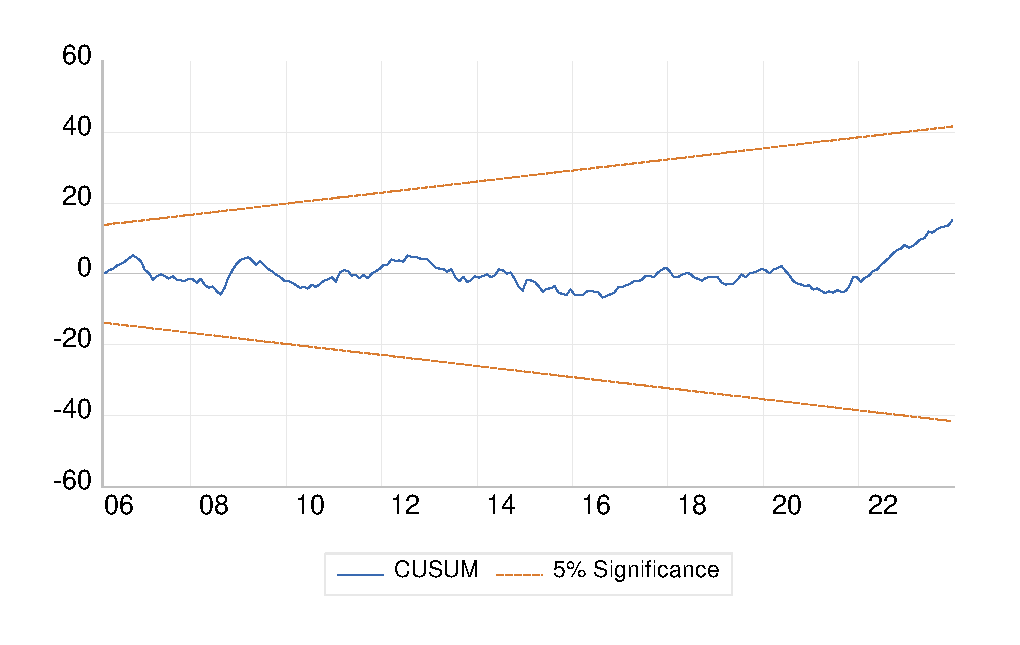
\includegraphics[scale=0.9]{annexes/cusum_nardl_logimm.pdf}
    \label{fig:msih_resids}
\end{figure}

\begin{figure}[H]
    \centering
    \caption{Test de normalité sur les résidus du modèle NARDL sur le LOGIMM.}
    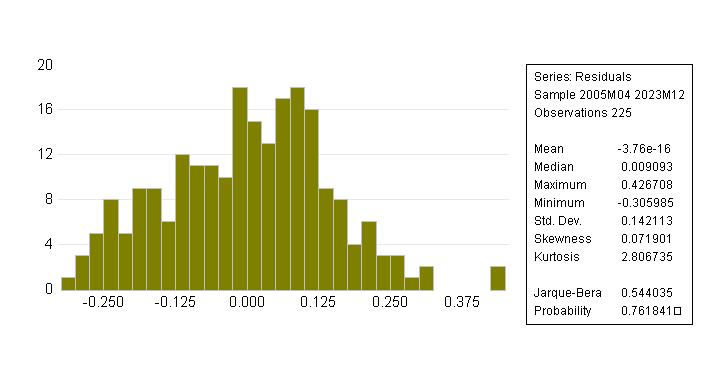
\includegraphics[scale=0.8]{annexes/normality_nardl_logimm.png}
    \label{fig:normalite_nardl_logimm}
\end{figure}

\begin{figure}[H]
    \centering
    \caption{Test d'autorrélation sur les résidus du modèle NARDL sur le LOGIMM.}
    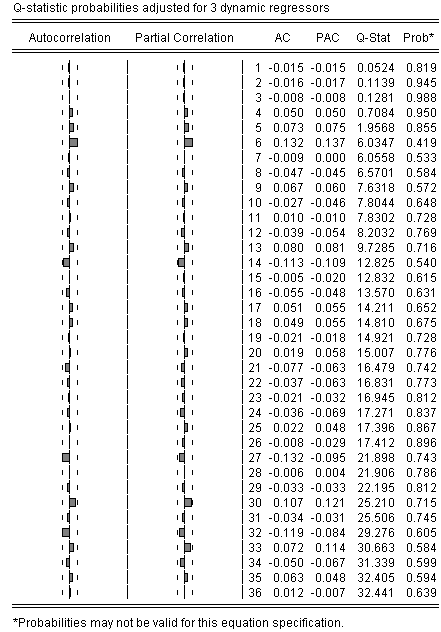
\includegraphics[scale=0.8]{annexes/correlogram_nardl_logimm.png}
    \label{fig:correlo_nardl_imm}
\end{figure}

\begin{table}[H]
    \centering
    \sffamily
    \caption{Test ARCH sur les résidus du modèle NARDL sur le LOGIMM.}
    \label{tab:arch_nardl_logimm}
    \resizebox{0.8\textwidth}{!}{\begin{tabular}{lrrrr}
\multicolumn{2}{l}{Heteroskedasticity Test: ARCH}&\multicolumn{1}{c}{}&\multicolumn{1}{c}{}&\multicolumn{1}{c}{}\\
[4.5pt] \hline \\ [-4.5pt]
\multicolumn{1}{l}{F-statistic}&\multicolumn{1}{r}{$0.398801$}&\multicolumn{2}{l}{Prob. F(10,204)}&\multicolumn{1}{r}{$0.9461$}\\
\multicolumn{1}{l}{Obs*R-squared}&\multicolumn{1}{r}{$4.122461$}&\multicolumn{2}{l}{Prob. Chi-Square(10)}&\multicolumn{1}{r}{$0.9417$}\\
[4.5pt] \hline \\ [-4.5pt]
\multicolumn{1}{c}{}&\multicolumn{1}{c}{}&\multicolumn{1}{c}{}&\multicolumn{1}{c}{}&\multicolumn{1}{c}{}\\
\multicolumn{1}{l}{Test Equation:}&\multicolumn{1}{c}{}&\multicolumn{1}{c}{}&\multicolumn{1}{c}{}&\multicolumn{1}{c}{}\\
\multicolumn{2}{l}{Dependent Variable: RESID\textasciicircum 2}&\multicolumn{1}{c}{}&\multicolumn{1}{c}{}&\multicolumn{1}{c}{}\\
\multicolumn{2}{l}{Method: Least Squares}&\multicolumn{1}{c}{}&\multicolumn{1}{c}{}&\multicolumn{1}{c}{}\\
\multicolumn{3}{l}{Sample (adjusted): 2006M02 2023M12}&\multicolumn{1}{c}{}&\multicolumn{1}{c}{}\\
\multicolumn{4}{l}{Included observations: 215 after adjustments}&\multicolumn{1}{c}{}\\
\multicolumn{6}{l}{HAC standard errors \& covariance}\\
{}&\multicolumn{1}{c}{}&\multicolumn{1}{c}{}\\
[4.5pt] \hline \\ [-4.5pt]
\multicolumn{1}{c}{Variable}&\multicolumn{1}{r}{Coefficient}&\multicolumn{1}{r}{Std. Error}&\multicolumn{1}{r}{t-Statistic}&\multicolumn{1}{r}{Prob.}\\
[4.5pt] \hline \\ [-4.5pt]
\multicolumn{1}{c}{C}&\multicolumn{1}{r}{$0.018258$}&\multicolumn{1}{r}{$0.004048$}&\multicolumn{1}{r}{$4.510838$}&\multicolumn{1}{r}{$0.0000$}\\
\multicolumn{1}{c}{RESID\textasciicircum 2(-1)}&\multicolumn{1}{r}{$0.030943$}&\multicolumn{1}{r}{$0.065730$}&\multicolumn{1}{r}{$0.470754$}&\multicolumn{1}{r}{$0.6383$}\\
\multicolumn{1}{c}{RESID\textasciicircum 2(-2)}&\multicolumn{1}{r}{$0.044582$}&\multicolumn{1}{r}{$0.071457$}&\multicolumn{1}{r}{$0.623905$}&\multicolumn{1}{r}{$0.5334$}\\
\multicolumn{1}{c}{RESID\textasciicircum 2(-3)}&\multicolumn{1}{r}{$0.030183$}&\multicolumn{1}{r}{$0.056093$}&\multicolumn{1}{r}{$0.538087$}&\multicolumn{1}{r}{$0.5911$}\\
\multicolumn{1}{c}{RESID\textasciicircum 2(-4)}&\multicolumn{1}{r}{$0.018190$}&\multicolumn{1}{r}{$0.070288$}&\multicolumn{1}{r}{$0.258790$}&\multicolumn{1}{r}{$0.7961$}\\
\multicolumn{1}{c}{RESID\textasciicircum 2(-5)}&\multicolumn{1}{r}{$0.012319$}&\multicolumn{1}{r}{$0.056729$}&\multicolumn{1}{r}{$0.217151$}&\multicolumn{1}{r}{$0.8283$}\\
\multicolumn{1}{c}{RESID\textasciicircum 2(-6)}&\multicolumn{1}{r}{$-0.009711$}&\multicolumn{1}{r}{$0.060427$}&\multicolumn{1}{r}{$-0.160709$}&\multicolumn{1}{r}{$0.8725$}\\
\multicolumn{1}{c}{RESID\textasciicircum 2(-7)}&\multicolumn{1}{r}{$-0.025220$}&\multicolumn{1}{r}{$0.050909$}&\multicolumn{1}{r}{$-0.495387$}&\multicolumn{1}{r}{$0.6209$}\\
\multicolumn{1}{c}{RESID\textasciicircum 2(-8)}&\multicolumn{1}{r}{$0.079311$}&\multicolumn{1}{r}{$0.071075$}&\multicolumn{1}{r}{$1.115873$}&\multicolumn{1}{r}{$0.2658$}\\
\multicolumn{1}{c}{RESID\textasciicircum 2(-9)}&\multicolumn{1}{r}{$-0.084982$}&\multicolumn{1}{r}{$0.046664$}&\multicolumn{1}{r}{$-1.821152$}&\multicolumn{1}{r}{$0.0700$}\\
\multicolumn{1}{c}{RESID\textasciicircum 2(-10)}&\multicolumn{1}{r}{$-0.023029$}&\multicolumn{1}{r}{$0.049464$}&\multicolumn{1}{r}{$-0.465568$}&\multicolumn{1}{r}{$0.6420$}\\
[4.5pt] \hline \\ [-4.5pt]
\multicolumn{1}{l}{R-squared}&\multicolumn{1}{r}{$0.019174$}&\multicolumn{2}{l}{Mean dependent var}&\multicolumn{1}{r}{$0.019635$}\\
\multicolumn{1}{l}{Adjusted R-squared}&\multicolumn{1}{r}{$-0.028905$}&\multicolumn{2}{l}{S.D. dependent var}&\multicolumn{1}{r}{$0.026870$}\\
\multicolumn{1}{l}{S.E. of regression}&\multicolumn{1}{r}{$0.027255$}&\multicolumn{2}{l}{Akaike info criterion}&\multicolumn{1}{r}{$-4.317326$}\\
\multicolumn{1}{l}{Sum squared resid}&\multicolumn{1}{r}{$0.151542$}&\multicolumn{2}{l}{Schwarz criterion}&\multicolumn{1}{r}{$-4.144874$}\\
\multicolumn{1}{l}{Log likelihood}&\multicolumn{1}{r}{$475.1125$}&\multicolumn{2}{l}{Hannan-Quinn criter.}&\multicolumn{1}{r}{$-4.247647$}\\
\multicolumn{1}{l}{F-statistic}&\multicolumn{1}{r}{$0.398801$}&\multicolumn{2}{l}{Durbin-Watson stat}&\multicolumn{1}{r}{$1.997920$}\\
\multicolumn{1}{l}{Prob(F-statistic)}&\multicolumn{1}{r}{$0.946145$}&\multicolumn{1}{c}{}&\multicolumn{1}{c}{}&\multicolumn{1}{c}{}\\
[4.5pt] \hline \\ [-4.5pt]
\end{tabular}}
\end{table}

\subsubsection{Estimation du modèle NARDL sur le marché actions}

\begin{table}[H]
    \centering
    \sffamily
    \caption{Estimation du modèle NARDL sur le LOGEQUITY.}
    \label{tab:nardl_logequity}
    \resizebox{0.8\textwidth}{!}{\begin{tabular}{lrrrr}
\multicolumn{3}{l}{Dependent Variable: LOGEQUITY}&\multicolumn{1}{c}{}&\multicolumn{1}{c}{}\\
\multicolumn{1}{l}{Method: ARDL}&\multicolumn{1}{c}{}&\multicolumn{1}{c}{}&\multicolumn{1}{c}{}&\multicolumn{1}{c}{}\\
\multicolumn{3}{l}{Sample (adjusted): 2005M06 2023M12}&\multicolumn{1}{c}{}&\multicolumn{1}{c}{}\\
\multicolumn{4}{l}{Included observations: 223 after adjustments}&\multicolumn{1}{c}{}\\
\multicolumn{4}{l}{Maximum dependent lags: 4 (Automatic selection)}&\multicolumn{1}{c}{}\\
\multicolumn{4}{l}{Model selection method: Akaike info criterion (AIC)}&\multicolumn{1}{c}{}\\
\multicolumn{4}{l}{Dynamic regressors : LOGIMM\_POS LOGIMM\_NEG}\\
\multicolumn{3}{l}{LOGFOREX\_POS LOGFOREX\_NEG}&\multicolumn{1}{c}{}&\multicolumn{1}{c}{}\\
\multicolumn{1}{l}{Fixed regressors: C}&\multicolumn{1}{c}{}&\multicolumn{1}{c}{}&\multicolumn{1}{c}{}&\multicolumn{1}{c}{}\\
\multicolumn{3}{l}{Number of models evaluated: 2500}&\multicolumn{1}{c}{}&\multicolumn{1}{c}{}\\
\multicolumn{3}{l}{Selected Model: ARDL(3, 1, 1, 4, 0)}&\multicolumn{1}{c}{}&\multicolumn{1}{c}{}\\
\multicolumn{6}{l}{HAC standard errors \& covariance}\\
\multicolumn{2}{l}{bandwidth = 5.0000)}&\multicolumn{1}{c}{}&\multicolumn{1}{c}{}&\multicolumn{1}{c}{}\\
[4.5pt] \hline \\ [-4.5pt]
\multicolumn{1}{c}{Variable}&\multicolumn{1}{r}{Coefficient}&\multicolumn{1}{r}{Std. Error}&\multicolumn{1}{r}{t-Statistic}&\multicolumn{1}{r}{Prob.*}\\
[4.5pt] \hline \\ [-4.5pt]
\multicolumn{1}{c}{LOGEQUITY(-1)}&\multicolumn{1}{r}{$0.463576$}&\multicolumn{1}{r}{$0.070888$}&\multicolumn{1}{r}{$6.539588$}&\multicolumn{1}{r}{$0.0000$}\\
\multicolumn{1}{c}{LOGEQUITY(-2)}&\multicolumn{1}{r}{$-0.025110$}&\multicolumn{1}{r}{$0.0064991$}&\multicolumn{1}{r}{$-3.86356$}&\multicolumn{1}{r}{$0.0002$}\\
\multicolumn{1}{c}{LOGEQUITY(-3)}&\multicolumn{1}{r}{$0.176925$}&\multicolumn{1}{r}{$0.060576$}&\multicolumn{1}{r}{$2.920687$}&\multicolumn{1}{r}{$0.0039$}\\
\multicolumn{1}{c}{LOGIMM\_POS}&\multicolumn{1}{r}{$0.653087$}&\multicolumn{1}{r}{$0.221923$}&\multicolumn{1}{r}{$2.942849$}&\multicolumn{1}{r}{$0.0036$}\\
\multicolumn{1}{c}{LOGIMM\_POS(-1)}&\multicolumn{1}{r}{$-0.474638$}&\multicolumn{1}{r}{$0.210703$}&\multicolumn{1}{r}{$-2.252646$}&\multicolumn{1}{r}{$0.0253$}\\
\multicolumn{1}{c}{LOGIMM\_NEG}&\multicolumn{1}{r}{$0.809071$}&\multicolumn{1}{r}{$0.175485$}&\multicolumn{1}{r}{$4.610485$}&\multicolumn{1}{r}{$0.0000$}\\
\multicolumn{1}{c}{LOGIMM\_NEG(-1)}&\multicolumn{1}{r}{$-0.617908$}&\multicolumn{1}{r}{$0.168148$}&\multicolumn{1}{r}{$-3.674793$}&\multicolumn{1}{r}{$0.0003$}\\
\multicolumn{1}{c}{LOGFOREX\_POS}&\multicolumn{1}{r}{$0.332573$}&\multicolumn{1}{r}{$0.098151$}&\multicolumn{1}{r}{$3.388394$}&\multicolumn{1}{r}{$0.0008$}\\
\multicolumn{1}{c}{LOGFOREX\_POS(-1)}&\multicolumn{1}{r}{$-0.075632$}&\multicolumn{1}{r}{$0.020755$}&\multicolumn{1}{r}{$-3.644038$}&\multicolumn{1}{r}{$0.0004$}\\
\multicolumn{1}{c}{LOGFOREX\_POS(-2)}&\multicolumn{1}{r}{$0.193545$}&\multicolumn{1}{r}{$0.096894$}&\multicolumn{1}{r}{$1.997487$}&\multicolumn{1}{r}{$0.0471$}\\
\multicolumn{1}{c}{LOGFOREX\_POS(-3)}&\multicolumn{1}{r}{$-0.133520$}&\multicolumn{1}{r}{$0.082747$}&\multicolumn{1}{r}{$-1.613595$}&\multicolumn{1}{r}{$0.1081$}\\
\multicolumn{1}{c}{LOGFOREX\_POS(-4)}&\multicolumn{1}{r}{$-0.099465$}&\multicolumn{1}{r}{$0.049839$}&\multicolumn{1}{r}{$-1.995742$}&\multicolumn{1}{r}{$0.0473$}\\
\multicolumn{1}{c}{LOGFOREX\_NEG}&\multicolumn{1}{r}{$0.207261$}&\multicolumn{1}{r}{$0.044550$}&\multicolumn{1}{r}{$4.652283$}&\multicolumn{1}{r}{$0.0000$}\\
\multicolumn{1}{c}{C}&\multicolumn{1}{r}{$0.364372$}&\multicolumn{1}{r}{$0.126090$}&\multicolumn{1}{r}{$2.889768$}&\multicolumn{1}{r}{$0.0043$}\\
[4.5pt] \hline \\ [-4.5pt]
\multicolumn{1}{l}{R-squared}&\multicolumn{1}{r}{$0.829592$}&\multicolumn{2}{l}{Mean dependent var}&\multicolumn{1}{r}{$1.928245$}\\
\multicolumn{1}{l}{Adjusted R-squared}&\multicolumn{1}{r}{$0.818993$}&\multicolumn{2}{l}{S.D. dependent var}&\multicolumn{1}{r}{$0.606578$}\\
\multicolumn{1}{l}{S.E. of regression}&\multicolumn{1}{r}{$0.258068$}&\multicolumn{2}{l}{Akaike info criterion}&\multicolumn{1}{r}{$0.189539$}\\
\multicolumn{1}{l}{Sum squared resid}&\multicolumn{1}{r}{$13.91925$}&\multicolumn{2}{l}{Schwarz criterion}&\multicolumn{1}{r}{$0.403442$}\\
\multicolumn{1}{l}{Log likelihood}&\multicolumn{1}{r}{$-7.133575$}&\multicolumn{2}{l}{Hannan-Quinn criter.}&\multicolumn{1}{r}{$0.275890$}\\
\multicolumn{1}{l}{F-statistic}&\multicolumn{1}{r}{$78.26701$}&\multicolumn{2}{l}{Durbin-Watson stat}&\multicolumn{1}{r}{$1.910624$}\\
\multicolumn{1}{l}{Prob(F-statistic)}&\multicolumn{1}{r}{$0.000000$}&\multicolumn{1}{c}{}&\multicolumn{1}{c}{}&\multicolumn{1}{c}{}\\
[4.5pt] \hline \\ [-4.5pt]
\multicolumn{1}{l}{selection.}&\multicolumn{1}{c}{}&\multicolumn{1}{c}{}&\multicolumn{1}{c}{}&\multicolumn{1}{c}{}\\
\end{tabular}}
\end{table}

\begin{table}[H]
    \centering
    \sffamily
    \caption{Test d'existence des asymétries sur le modèle NARDL LOGEQUITY.}
    \label{tab:asymetrie_nardl_logequity}
    \resizebox{0.8\textwidth}{!}{\begin{tabular}{lrrr}
\multicolumn{1}{l}{Wald Test:}&\multicolumn{1}{c}{}&\multicolumn{1}{c}{}&\multicolumn{1}{c}{}\\
\multicolumn{2}{l}{Equation: NARDL03}&\multicolumn{1}{c}{}&\multicolumn{1}{c}{}\\
[4.5pt] \hline \\ [-4.5pt]
\multicolumn{1}{l}{Test Statistic}&\multicolumn{1}{c}{Value}&\multicolumn{1}{c}{df}&\multicolumn{1}{c}{Probability}\\
[4.5pt] \hline \\ [-4.5pt]
\multicolumn{1}{l}{F-statistic}&\multicolumn{1}{c}{$3.150231$}&\multicolumn{1}{c}{(7, 209)}&\multicolumn{1}{c}{$0.0035$}\\
\multicolumn{1}{l}{Chi-square}&\multicolumn{1}{c}{$22.05162$}&\multicolumn{1}{c}{$7$}&\multicolumn{1}{c}{$0.0025$}\\
[4.5pt] \hline \\ [-4.5pt]
\multicolumn{1}{c}{}&\multicolumn{1}{c}{}&\multicolumn{1}{c}{}&\multicolumn{1}{c}{}\\
\multicolumn{5}{l}{Null Hypothesis: C(4) = C(9), C(5) = 0, C(6) = 0, C(7) = 0,}\\
\multicolumn{3}{l}{C(8) =0, C(10) = C(12), C(11) = C(13)}&\multicolumn{1}{c}{}\\
\multicolumn{2}{l}{Null Hypothesis Summary:}&\multicolumn{1}{c}{}&\multicolumn{1}{c}{}\\
[4.5pt] \hline \\ [-4.5pt]
\multicolumn{2}{l}{Normalized Restriction (= 0)}&\multicolumn{1}{c}{Value}&\multicolumn{1}{c}{Std. Err.}\\
[4.5pt] \hline \\ [-4.5pt]
\multicolumn{1}{l}{C(4) - C(9)}&\multicolumn{1}{c}{}&\multicolumn{1}{c}{$0.125312$}&\multicolumn{1}{c}{$0.094158$}\\
\multicolumn{1}{l}{C(5)}&\multicolumn{1}{c}{}&\multicolumn{1}{c}{$-0.075632$}&\multicolumn{1}{c}{$0.120755$}\\
\multicolumn{1}{l}{C(6)}&\multicolumn{1}{c}{}&\multicolumn{1}{c}{$0.193545$}&\multicolumn{1}{c}{$0.096894$}\\
\multicolumn{1}{l}{C(7)}&\multicolumn{1}{c}{}&\multicolumn{1}{c}{$-0.133520$}&\multicolumn{1}{c}{$0.082747$}\\
\multicolumn{1}{l}{C(8)}&\multicolumn{1}{c}{}&\multicolumn{1}{c}{$-0.099465$}&\multicolumn{1}{c}{$0.049839$}\\
\multicolumn{1}{l}{C(10) - C(12)}&\multicolumn{1}{c}{}&\multicolumn{1}{c}{$-0.155984$}&\multicolumn{1}{c}{$0.328076$}\\
\multicolumn{1}{l}{C(11) - C(13)}&\multicolumn{1}{c}{}&\multicolumn{1}{c}{$0.143270$}&\multicolumn{1}{c}{$0.318155$}\\
[4.5pt] \hline \\ [-4.5pt]
\multicolumn{3}{l}{Restrictions are linear in coefficients.}&\multicolumn{1}{c}{}\\
\end{tabular}
}
\end{table}

\begin{table}[H]
    \centering
    \sffamily
    \caption{Test de multicolinéarité (VIF) sur le modèle NARDL LOGEQUITY.}
    \label{tab:vif_nardl_logequity}
    \resizebox{0.8\textwidth}{!}{\begin{tabular}{lrrr}
\multicolumn{2}{l}{Variance Inflation Factors}&\multicolumn{1}{c}{}&\multicolumn{1}{c}{}\\
\multicolumn{2}{l}{Sample: 2005M01 2023M12}&\multicolumn{1}{c}{}&\multicolumn{1}{c}{}\\
\multicolumn{2}{l}{Included observations: 223}&\multicolumn{1}{c}{}&\multicolumn{1}{c}{}\\
[4.5pt] \hline \\ [-4.5pt]
\multicolumn{1}{c}{}&\multicolumn{1}{c}{Coefficient}&\multicolumn{1}{c}{Uncentered}&\multicolumn{1}{c}{Centered}\\
\multicolumn{1}{c}{Variable}&\multicolumn{1}{c}{Variance}&\multicolumn{1}{c}{VIF}&\multicolumn{1}{c}{VIF}\\
[4.5pt] \hline \\ [-4.5pt]
\multicolumn{1}{c}{LOGEQUITY(-1)}&\multicolumn{1}{c}{$0.005025$}&\multicolumn{1}{c}{$89.62473$}&\multicolumn{1}{c}{$6.766383$}\\
\multicolumn{1}{c}{LOGEQUITY(-2)}&\multicolumn{1}{c}{$0.004224$}&\multicolumn{1}{c}{$76.78250$}&\multicolumn{1}{c}{$6.779116$}\\
\multicolumn{1}{c}{LOGEQUITY(-3)}&\multicolumn{1}{c}{$0.003669$}&\multicolumn{1}{c}{$62.46960$}&\multicolumn{1}{c}{$4.618255$}\\
\multicolumn{1}{c}{LOGFOREX\_POS}&\multicolumn{1}{c}{$0.009634$}&\multicolumn{1}{c}{$18212.75$}&\multicolumn{1}{c}{$3696.508$}\\
\multicolumn{1}{c}{LOGFOREX\_POS(-1)}&\multicolumn{1}{c}{$0.014582$}&\multicolumn{1}{c}{$27125.81$}&\multicolumn{1}{c}{$5558.469$}\\
\multicolumn{1}{c}{LOGFOREX\_POS(-2)}&\multicolumn{1}{c}{$0.009389$}&\multicolumn{1}{c}{$17230.83$}&\multicolumn{1}{c}{$3570.633$}\\
\multicolumn{1}{c}{LOGFOREX\_POS(-3)}&\multicolumn{1}{c}{$0.006847$}&\multicolumn{1}{c}{$12286.82$}&\multicolumn{1}{c}{$2598.632$}\\
\multicolumn{1}{c}{LOGFOREX\_POS(-4)}&\multicolumn{1}{c}{$0.002484$}&\multicolumn{1}{c}{$4373.763$}&\multicolumn{1}{c}{$954.6576$}\\
\multicolumn{1}{c}{LOGFOREX\_NEG}&\multicolumn{1}{c}{$0.001985$}&\multicolumn{1}{c}{$3632.116$}&\multicolumn{1}{c}{$781.0605$}\\
\multicolumn{1}{c}{LOGIMM\_POS}&\multicolumn{1}{c}{$0.049250$}&\multicolumn{1}{c}{$26700.66$}&\multicolumn{1}{c}{$4457.927$}\\
\multicolumn{1}{c}{LOGIMM\_POS(-1)}&\multicolumn{1}{c}{$0.044396$}&\multicolumn{1}{c}{$23771.50$}&\multicolumn{1}{c}{$4033.966$}\\
\multicolumn{1}{c}{LOGIMM\_NEG}&\multicolumn{1}{c}{$0.030795$}&\multicolumn{1}{c}{$15092.43$}&\multicolumn{1}{c}{$3026.259$}\\
\multicolumn{1}{c}{LOGIMM\_NEG(-1)}&\multicolumn{1}{c}{$0.028274$}&\multicolumn{1}{c}{$13698.95$}&\multicolumn{1}{c}{$2775.918$}\\
\multicolumn{1}{c}{C}&\multicolumn{1}{c}{$0.015899$}&\multicolumn{1}{c}{$67.19360$}&\multicolumn{1}{c}{$NA$}\\
[4.5pt] \hline \\ [-4.5pt]
\end{tabular}}
\end{table}

\begin{table}[H]
    \centering
    \sffamily
    \caption{Test de redondance des variables asymétriques dans le modèle NARDL LOGEQUITY.}
    \label{tab:redondance_nardl_logequity}
    \resizebox{1\textwidth}{!}{\begin{tabular}{lrrrr}
\multicolumn{2}{l}{Redundant Variables Test}&\multicolumn{1}{c}{}&\multicolumn{1}{c}{}&\multicolumn{1}{c}{}\\
\multicolumn{1}{l}{Equation: NARDL03}&\multicolumn{1}{c}{}&\multicolumn{1}{c}{}&\multicolumn{1}{c}{}&\multicolumn{1}{c}{}\\
\multicolumn{5}{l}{Redundant variables: LOGFOREX\_POS LOGFOREX\_POS(-1)}\\
\multicolumn{6}{l}{LOGFOREX\_POS(-2) LOGFOREX\_POS(-3) LOGFOREX\_POS(-4)}\\
\multicolumn{6}{l}{LOGFOREX\_NEG LOGIMM\_POS LOGIMM\_POS(-1) LOGIMM\_NEG}\\
\multicolumn{2}{l}{LOGIMM\_NEG(-1)}&\multicolumn{1}{c}{}&\multicolumn{1}{c}{}&\multicolumn{1}{c}{}\\
\multicolumn{6}{l}{Specification: LOGEQUITY LOGEQUITY(-1) LOGEQUITY(-2) LOGEQUITY(}\\
\multicolumn{6}{l}{-3) LOGFOREX\_POS LOGFOREX\_POS(-1) LOGFOREX\_POS(-2)}\\
\multicolumn{5}{l}{LOGFOREX\_POS(-3) LOGFOREX\_POS(-4) LOGFOREX\_NEG}\\
\multicolumn{6}{l}{LOGIMM\_POS LOGIMM\_POS(-1) LOGIMM\_NEG LOGIMM\_NEG(-1) C}\\
\multicolumn{5}{l}{Null hypothesis: LOGFOREX\_POS LOGFOREX\_POS(-1)}\\
\multicolumn{6}{l}{LOGFOREX\_POS(-2) LOGFOREX\_POS(-3) LOGFOREX\_POS(-4)}\\
\multicolumn{6}{l}{LOGFOREX\_NEG LOGIMM\_POS LOGIMM\_POS(-1) LOGIMM\_NEG}\\
\multicolumn{4}{l}{LOGIMM\_NEG(-1)   are jointly insignificant}&\multicolumn{1}{c}{}\\
[4.5pt] \hline \\ [-4.5pt]
\multicolumn{1}{c}{}&\multicolumn{1}{c}{Value}&\multicolumn{1}{c}{df}&\multicolumn{1}{c}{Probability}&\multicolumn{1}{c}{}\\
\multicolumn{1}{l}{F-statistic}&\multicolumn{1}{c}{$19.49109$}&\multicolumn{1}{c}{(10, 209)}&\multicolumn{1}{c}{$0.0000$}&\multicolumn{1}{c}{}\\
[4.5pt] \hline \\ [-4.5pt]
\multicolumn{1}{l}{F-test summary:}&\multicolumn{1}{c}{}&\multicolumn{1}{c}{}&\multicolumn{1}{c}{}&\multicolumn{1}{c}{}\\
\multicolumn{1}{c}{}&\multicolumn{1}{c}{Sum of Sq.}&\multicolumn{1}{c}{df}&\multicolumn{1}{c}{Mean Squares}&\multicolumn{1}{c}{}\\
\multicolumn{1}{l}{Test SSR}&\multicolumn{1}{c}{$12.98093$}&\multicolumn{1}{c}{$10$}&\multicolumn{1}{c}{$1.298093$}&\multicolumn{1}{c}{}\\
\multicolumn{1}{l}{Restricted SSR}&\multicolumn{1}{c}{$26.90018$}&\multicolumn{1}{c}{$219$}&\multicolumn{1}{c}{$0.122832$}&\multicolumn{1}{c}{}\\
\multicolumn{1}{l}{Unrestricted SSR}&\multicolumn{1}{c}{$13.91925$}&\multicolumn{1}{c}{$209$}&\multicolumn{1}{c}{$0.066599$}&\multicolumn{1}{c}{}\\
[4.5pt] \hline \\ [-4.5pt]
\multicolumn{1}{c}{}&\multicolumn{1}{c}{}&\multicolumn{1}{c}{}&\multicolumn{1}{c}{}&\multicolumn{1}{c}{}\\
\multicolumn{2}{l}{Restricted Test Equation:}&\multicolumn{1}{c}{}&\multicolumn{1}{c}{}&\multicolumn{1}{c}{}\\
\multicolumn{3}{l}{Dependent Variable: LOGEQUITY}&\multicolumn{1}{c}{}&\multicolumn{1}{c}{}\\
\multicolumn{2}{l}{Method: Least Squares}&\multicolumn{1}{c}{}&\multicolumn{1}{c}{}&\multicolumn{1}{c}{}\\
\multicolumn{2}{l}{Sample: 2005M06 2023M12}&\multicolumn{1}{c}{}&\multicolumn{1}{c}{}&\multicolumn{1}{c}{}\\
\multicolumn{2}{l}{Included observations: 223}&\multicolumn{1}{c}{}&\multicolumn{1}{c}{}&\multicolumn{1}{c}{}\\
\multicolumn{6}{l}{HAC standard errors \& covariance (Bartlett kernel, Newey-West fixed}\\
\multicolumn{2}{l}{bandwidth = 5.0000)}&\multicolumn{1}{c}{}&\multicolumn{1}{c}{}&\multicolumn{1}{c}{}\\
[4.5pt] \hline \\ [-4.5pt]
\multicolumn{1}{c}{Variable}&\multicolumn{1}{r}{Coefficient}&\multicolumn{1}{r}{Std. Error}&\multicolumn{1}{r}{t-Statistic}&\multicolumn{1}{r}{Prob.}\\
[4.5pt] \hline \\ [-4.5pt]
\multicolumn{1}{c}{LOGEQUITY(-1)}&\multicolumn{1}{r}{$0.617751$}&\multicolumn{1}{r}{$0.085943$}&\multicolumn{1}{r}{$7.187926$}&\multicolumn{1}{r}{$0.0000$}\\
\multicolumn{1}{c}{LOGEQUITY(-2)}&\multicolumn{1}{r}{$0.088479$}&\multicolumn{1}{r}{$0.087108$}&\multicolumn{1}{r}{$1.015741$}&\multicolumn{1}{r}{$0.3109$}\\
\multicolumn{1}{c}{LOGEQUITY(-3)}&\multicolumn{1}{r}{$0.157484$}&\multicolumn{1}{r}{$0.066559$}&\multicolumn{1}{r}{$2.366097$}&\multicolumn{1}{r}{$0.0188$}\\
\multicolumn{1}{c}{C}&\multicolumn{1}{r}{$0.265545$}&\multicolumn{1}{r}{$0.078284$}&\multicolumn{1}{r}{$3.392089$}&\multicolumn{1}{r}{$0.0008$}\\
[4.5pt] \hline \\ [-4.5pt]
\multicolumn{1}{l}{R-squared}&\multicolumn{1}{r}{$0.670672$}&\multicolumn{2}{l}{Mean dependent var}&\multicolumn{1}{r}{$1.928245$}\\
\multicolumn{1}{l}{Adjusted R-squared}&\multicolumn{1}{r}{$0.666161$}&\multicolumn{2}{l}{S.D. dependent var}&\multicolumn{1}{r}{$0.606578$}\\
\multicolumn{1}{l}{S.E. of regression}&\multicolumn{1}{r}{$0.350474$}&\multicolumn{2}{l}{Akaike info criterion}&\multicolumn{1}{r}{$0.758713$}\\
\multicolumn{1}{l}{Sum squared resid}&\multicolumn{1}{r}{$26.90018$}&\multicolumn{2}{l}{Schwarz criterion}&\multicolumn{1}{r}{$0.819828$}\\
\multicolumn{1}{l}{Log likelihood}&\multicolumn{1}{r}{$-80.59648$}&\multicolumn{2}{l}{Hannan-Quinn criter.}&\multicolumn{1}{r}{$0.783385$}\\
\multicolumn{1}{l}{F-statistic}&\multicolumn{1}{r}{$148.6637$}&\multicolumn{2}{l}{Durbin-Watson stat}&\multicolumn{1}{r}{$1.964152$}\\
\multicolumn{1}{l}{Prob(F-statistic)}&\multicolumn{1}{r}{$0.000000$}&\multicolumn{2}{l}{Wald F-statistic}&\multicolumn{1}{r}{$203.4881$}\\
\multicolumn{1}{l}{Prob(Wald F-statistic)}&\multicolumn{1}{r}{$0.000000$}&\multicolumn{1}{c}{}&\multicolumn{1}{c}{}&\multicolumn{1}{c}{}\\
[4.5pt] \hline \\ [-4.5pt]
\end{tabular}
}
\end{table}

\begin{table}[H]
    \centering
    \sffamily
    \caption{Test RESET de Ramsey dans le modèle NARDL LOGEQUITY.}
    \label{tab:reset_nardl_logequity}
    \resizebox{1\textwidth}{!}{\begin{tabular}{lrrrr}
\multicolumn{1}{l}{Ramsey RESET Test}&\multicolumn{1}{c}{}&\multicolumn{1}{c}{}&\multicolumn{1}{c}{}&\multicolumn{1}{c}{}\\
\multicolumn{1}{l}{Equation: NARDL03}&\multicolumn{1}{c}{}&\multicolumn{1}{c}{}&\multicolumn{1}{c}{}&\multicolumn{1}{c}{}\\
\multicolumn{3}{l}{Omitted Variables: Squares of fitted values}&\multicolumn{1}{c}{}&\multicolumn{1}{c}{}\\
\multicolumn{6}{l}{Specification: LOGEQUITY LOGEQUITY(-1) LOGEQUITY(-2) LOGEQUITY(}\\
\multicolumn{6}{l}{-3) LOGFOREX\_POS LOGFOREX\_POS(-1) LOGFOREX\_POS(-2)}\\
\multicolumn{5}{l}{LOGFOREX\_POS(-3) LOGFOREX\_POS(-4) LOGFOREX\_NEG}\\
\multicolumn{6}{l}{LOGIMM\_POS LOGIMM\_POS(-1) LOGIMM\_NEG LOGIMM\_NEG(-1) C}\\
[4.5pt] \hline \\ [-4.5pt]
\multicolumn{1}{c}{}&\multicolumn{1}{c}{Value}&\multicolumn{1}{c}{df}&\multicolumn{1}{c}{Probability}&\multicolumn{1}{c}{}\\
\multicolumn{1}{l}{t-statistic}&\multicolumn{1}{c}{$0.727348$}&\multicolumn{1}{c}{$208$}&\multicolumn{1}{c}{$0.4678$}&\multicolumn{1}{c}{}\\
\multicolumn{1}{l}{F-statistic}&\multicolumn{1}{c}{$0.529035$}&\multicolumn{1}{c}{(1, 208)}&\multicolumn{1}{c}{$0.4678$}&\multicolumn{1}{c}{}\\
\multicolumn{1}{l}{Likelihood ratio}&\multicolumn{1}{c}{$0.566466$}&\multicolumn{1}{c}{$1$}&\multicolumn{1}{c}{$0.4517$}&\multicolumn{1}{c}{}\\
[4.5pt] \hline \\ [-4.5pt]
\multicolumn{1}{l}{F-test summary:}&\multicolumn{1}{c}{}&\multicolumn{1}{c}{}&\multicolumn{1}{c}{}&\multicolumn{1}{c}{}\\
\multicolumn{1}{c}{}&\multicolumn{1}{c}{Sum of Sq.}&\multicolumn{1}{c}{df}&\multicolumn{1}{c}{Mean Squares}&\multicolumn{1}{c}{}\\
\multicolumn{1}{l}{Test SSR}&\multicolumn{1}{c}{$0.035313$}&\multicolumn{1}{c}{$1$}&\multicolumn{1}{c}{$0.035313$}&\multicolumn{1}{c}{}\\
\multicolumn{1}{l}{Restricted SSR}&\multicolumn{1}{c}{$13.91925$}&\multicolumn{1}{c}{$209$}&\multicolumn{1}{c}{$0.066599$}&\multicolumn{1}{c}{}\\
\multicolumn{1}{l}{Unrestricted SSR}&\multicolumn{1}{c}{$13.88394$}&\multicolumn{1}{c}{$208$}&\multicolumn{1}{c}{$0.066750$}&\multicolumn{1}{c}{}\\
[4.5pt] \hline \\ [-4.5pt]
\multicolumn{1}{l}{LR test summary:}&\multicolumn{1}{c}{}&\multicolumn{1}{c}{}&\multicolumn{1}{c}{}&\multicolumn{1}{c}{}\\
\multicolumn{1}{c}{}&\multicolumn{1}{c}{Value}&\multicolumn{1}{c}{}&\multicolumn{1}{c}{}&\multicolumn{1}{c}{}\\
\multicolumn{1}{l}{Restricted LogL}&\multicolumn{1}{c}{$-7.133575$}&\multicolumn{1}{c}{}&\multicolumn{1}{c}{}&\multicolumn{1}{c}{}\\
\multicolumn{1}{l}{Unrestricted LogL}&\multicolumn{1}{c}{$-6.850342$}&\multicolumn{1}{c}{}&\multicolumn{1}{c}{}&\multicolumn{1}{c}{}\\
[4.5pt] \hline \\ [-4.5pt]
\multicolumn{1}{c}{}&\multicolumn{1}{c}{}&\multicolumn{1}{c}{}&\multicolumn{1}{c}{}&\multicolumn{1}{c}{}\\
\multicolumn{2}{l}{Unrestricted Test Equation:}&\multicolumn{1}{c}{}&\multicolumn{1}{c}{}&\multicolumn{1}{c}{}\\
\multicolumn{3}{l}{Dependent Variable: LOGEQUITY}&\multicolumn{1}{c}{}&\multicolumn{1}{c}{}\\
\multicolumn{2}{l}{Method: Least Squares}&\multicolumn{1}{c}{}&\multicolumn{1}{c}{}&\multicolumn{1}{c}{}\\
\multicolumn{2}{l}{Sample: 2005M06 2023M12}&\multicolumn{1}{c}{}&\multicolumn{1}{c}{}&\multicolumn{1}{c}{}\\
\multicolumn{2}{l}{Included observations: 223}&\multicolumn{1}{c}{}&\multicolumn{1}{c}{}&\multicolumn{1}{c}{}\\
\multicolumn{6}{l}{HAC standard errors \& covariance (Bartlett kernel, Newey-West fixed}\\
\multicolumn{2}{l}{bandwidth = 5.0000)}&\multicolumn{1}{c}{}&\multicolumn{1}{c}{}&\multicolumn{1}{c}{}\\
[4.5pt] \hline \\ [-4.5pt]
\multicolumn{1}{c}{Variable}&\multicolumn{1}{r}{Coefficient}&\multicolumn{1}{r}{Std. Error}&\multicolumn{1}{r}{t-Statistic}&\multicolumn{1}{r}{Prob.}\\
[4.5pt] \hline \\ [-4.5pt]
\multicolumn{1}{c}{LOGEQUITY(-1)}&\multicolumn{1}{r}{$0.529799$}&\multicolumn{1}{r}{$0.135150$}&\multicolumn{1}{r}{$3.920087$}&\multicolumn{1}{r}{$0.0001$}\\
\multicolumn{1}{c}{LOGEQUITY(-2)}&\multicolumn{1}{r}{$-0.021647$}&\multicolumn{1}{r}{$0.065149$}&\multicolumn{1}{r}{$-0.332273$}&\multicolumn{1}{r}{$0.7400$}\\
\multicolumn{1}{c}{LOGEQUITY(-3)}&\multicolumn{1}{r}{$0.201077$}&\multicolumn{1}{r}{$0.073221$}&\multicolumn{1}{r}{$2.746183$}&\multicolumn{1}{r}{$0.0066$}\\
\multicolumn{1}{c}{LOGFOREX\_POS}&\multicolumn{1}{r}{$0.374842$}&\multicolumn{1}{r}{$0.129600$}&\multicolumn{1}{r}{$2.892291$}&\multicolumn{1}{r}{$0.0042$}\\
\multicolumn{1}{c}{LOGFOREX\_POS(-1)}&\multicolumn{1}{r}{$-0.076820$}&\multicolumn{1}{r}{$0.120696$}&\multicolumn{1}{r}{$-0.636479$}&\multicolumn{1}{r}{$0.5252$}\\
\multicolumn{1}{c}{LOGFOREX\_POS(-2)}&\multicolumn{1}{r}{$0.218708$}&\multicolumn{1}{r}{$0.103135$}&\multicolumn{1}{r}{$2.120597$}&\multicolumn{1}{r}{$0.0351$}\\
\multicolumn{1}{c}{LOGFOREX\_POS(-3)}&\multicolumn{1}{r}{$-0.154715$}&\multicolumn{1}{r}{$0.084917$}&\multicolumn{1}{r}{$-1.821954$}&\multicolumn{1}{r}{$0.0699$}\\
\multicolumn{1}{c}{LOGFOREX\_POS(-4)}&\multicolumn{1}{r}{$-0.114218$}&\multicolumn{1}{r}{$0.054508$}&\multicolumn{1}{r}{$-2.095447$}&\multicolumn{1}{r}{$0.0373$}\\
\multicolumn{1}{c}{LOGFOREX\_NEG}&\multicolumn{1}{r}{$0.234729$}&\multicolumn{1}{r}{$0.072677$}&\multicolumn{1}{r}{$3.229769$}&\multicolumn{1}{r}{$0.0014$}\\
\multicolumn{1}{c}{LOGIMM\_POS}&\multicolumn{1}{r}{$0.785374$}&\multicolumn{1}{r}{$0.299047$}&\multicolumn{1}{r}{$2.626258$}&\multicolumn{1}{r}{$0.0093$}\\
\multicolumn{1}{c}{LOGIMM\_POS(-1)}&\multicolumn{1}{r}{$-0.569314$}&\multicolumn{1}{r}{$0.274158$}&\multicolumn{1}{r}{$-2.076589$}&\multicolumn{1}{r}{$0.0391$}\\
\multicolumn{1}{c}{LOGIMM\_NEG}&\multicolumn{1}{r}{$0.934707$}&\multicolumn{1}{r}{$0.225839$}&\multicolumn{1}{r}{$4.138816$}&\multicolumn{1}{r}{$0.0001$}\\
\multicolumn{1}{c}{LOGIMM\_NEG(-1)}&\multicolumn{1}{r}{$-0.700899$}&\multicolumn{1}{r}{$0.202031$}&\multicolumn{1}{r}{$-3.469275$}&\multicolumn{1}{r}{$0.0006$}\\
\multicolumn{1}{c}{C}&\multicolumn{1}{r}{$0.290914$}&\multicolumn{1}{r}{$0.168282$}&\multicolumn{1}{r}{$1.728729$}&\multicolumn{1}{r}{$0.0853$}\\
\multicolumn{1}{c}{FITTED\textasciicircum 2}&\multicolumn{1}{r}{$-0.041553$}&\multicolumn{1}{r}{$0.064154$}&\multicolumn{1}{r}{$-0.647702$}&\multicolumn{1}{r}{$0.5179$}\\
[4.5pt] \hline \\ [-4.5pt]
\multicolumn{1}{l}{R-squared}&\multicolumn{1}{r}{$0.830025$}&\multicolumn{2}{l}{Mean dependent var}&\multicolumn{1}{r}{$1.928245$}\\
\multicolumn{1}{l}{Adjusted R-squared}&\multicolumn{1}{r}{$0.818584$}&\multicolumn{2}{l}{S.D. dependent var}&\multicolumn{1}{r}{$0.606578$}\\
\multicolumn{1}{l}{S.E. of regression}&\multicolumn{1}{r}{$0.258360$}&\multicolumn{2}{l}{Akaike info criterion}&\multicolumn{1}{r}{$0.195967$}\\
\multicolumn{1}{l}{Sum squared resid}&\multicolumn{1}{r}{$13.88394$}&\multicolumn{2}{l}{Schwarz criterion}&\multicolumn{1}{r}{$0.425149$}\\
\multicolumn{1}{l}{Log likelihood}&\multicolumn{1}{r}{$-6.850342$}&\multicolumn{2}{l}{Hannan-Quinn criter.}&\multicolumn{1}{r}{$0.288486$}\\
\multicolumn{1}{l}{F-statistic}&\multicolumn{1}{r}{$72.55053$}&\multicolumn{2}{l}{Durbin-Watson stat}&\multicolumn{1}{r}{$1.905886$}\\
\multicolumn{1}{l}{Prob(F-statistic)}&\multicolumn{1}{r}{$0.000000$}&\multicolumn{2}{l}{Wald F-statistic}&\multicolumn{1}{r}{$97.23107$}\\
\multicolumn{1}{l}{Prob(Wald F-statistic)}&\multicolumn{1}{r}{$0.000000$}&\multicolumn{1}{c}{}&\multicolumn{1}{c}{}&\multicolumn{1}{c}{}\\
[4.5pt] \hline \\ [-4.5pt]
\end{tabular}
}
\end{table}

\begin{figure}[H]
    \centering
    \caption{Test de CUSUM du modèle NARDL sur le LOGEQUITY.}
    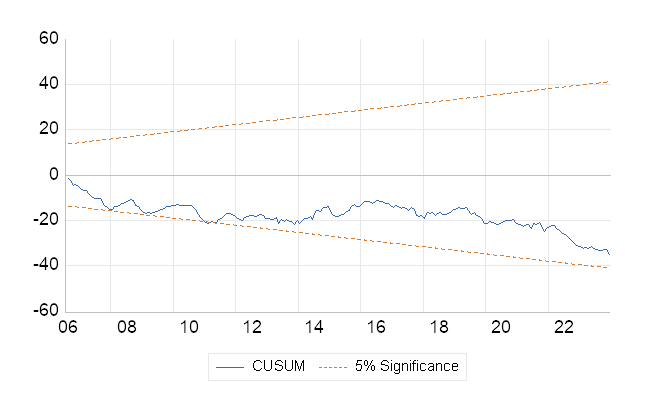
\includegraphics[scale=0.9]{annexes/cusum_nardl_logequity.png}
    \label{fig:msih_resids}
\end{figure}

\begin{figure}[H]
    \centering
    \caption{Test de normalité sur les résidus du modèle NARDL sur le LOGEQUITY.}
    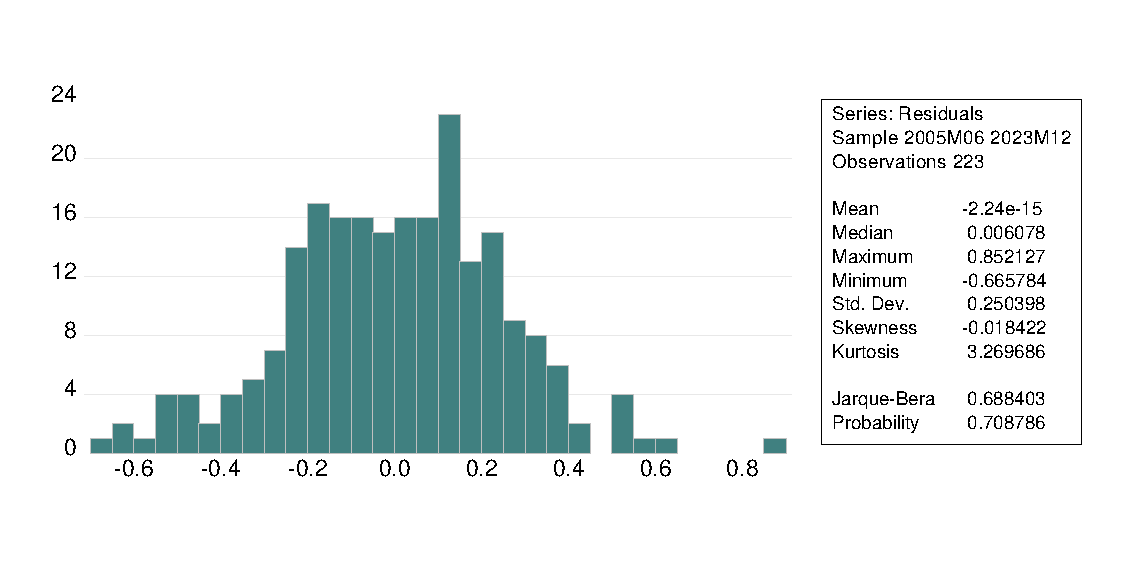
\includegraphics[scale=0.8]{annexes/normalite_nardl_logequity.pdf}
    \label{fig:normalite_nardl_logequity}
\end{figure}

\begin{figure}[H]
    \centering
    \caption{Test d'autorrélation sur les résidus du modèle NARDL sur le LOGEQUITY.}
    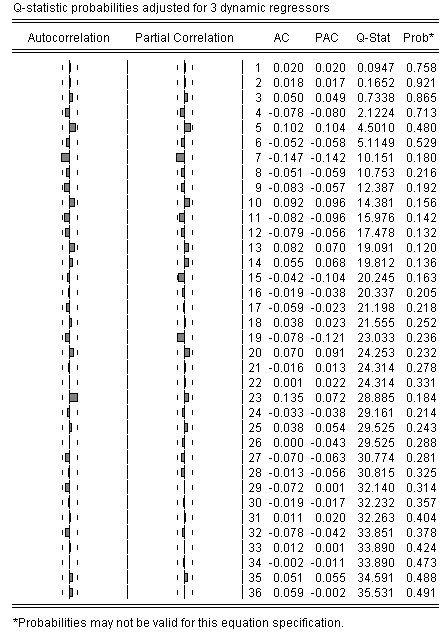
\includegraphics[scale=0.8]{annexes/autorrelation_nardl_logequity.png}
    \label{fig:correlo_nardl_equity}
\end{figure}

\begin{table}[H]
    \centering
    \sffamily
    \caption{Test ARCH sur les résidus du modèle NARDL sur le LOGEQUITY.}
    \label{tab:arch_nardl_logequity}
    \resizebox{0.8\textwidth}{!}{\begin{tabular}{lrrrr}
\multicolumn{2}{l}{Heteroskedasticity Test: ARCH}&\multicolumn{1}{c}{}&\multicolumn{1}{c}{}&\multicolumn{1}{c}{}\\
[4.5pt] \hline \\ [-4.5pt]
\multicolumn{1}{l}{F-statistic}&\multicolumn{1}{r}{$1.520254$}&\multicolumn{2}{l}{Prob. F(10,202)}&\multicolumn{1}{r}{$0.1341$}\\
\multicolumn{1}{l}{Obs*R-squared}&\multicolumn{1}{r}{$14.90839$}&\multicolumn{2}{l}{Prob. Chi-Square(10)}&\multicolumn{1}{r}{$0.1354$}\\
[4.5pt] \hline \\ [-4.5pt]
\multicolumn{1}{c}{}&\multicolumn{1}{c}{}&\multicolumn{1}{c}{}&\multicolumn{1}{c}{}&\multicolumn{1}{c}{}\\
\multicolumn{1}{l}{Test Equation:}&\multicolumn{1}{c}{}&\multicolumn{1}{c}{}&\multicolumn{1}{c}{}&\multicolumn{1}{c}{}\\
\multicolumn{2}{l}{Dependent Variable: RESID\textasciicircum 2}&\multicolumn{1}{c}{}&\multicolumn{1}{c}{}&\multicolumn{1}{c}{}\\
\multicolumn{2}{l}{Method: Least Squares}&\multicolumn{1}{c}{}&\multicolumn{1}{c}{}&\multicolumn{1}{c}{}\\
\multicolumn{3}{l}{Sample (adjusted): 2006M04 2023M12}&\multicolumn{1}{c}{}&\multicolumn{1}{c}{}\\
\multicolumn{4}{l}{Included observations: 213 after adjustments}&\multicolumn{1}{c}{}\\
\multicolumn{6}{l}{HAC standard errors \& covariance}\\
\multicolumn{2}{l}{bandwidth = 5.0000)}&\multicolumn{1}{c}{}&\multicolumn{1}{c}{}&\multicolumn{1}{c}{}\\
[4.5pt] \hline \\ [-4.5pt]
\multicolumn{1}{c}{Variable}&\multicolumn{1}{r}{Coefficient}&\multicolumn{1}{r}{Std. Error}&\multicolumn{1}{r}{t-Statistic}&\multicolumn{1}{r}{Prob.}\\
[4.5pt] \hline \\ [-4.5pt]
\multicolumn{1}{c}{C}&\multicolumn{1}{r}{$0.042386$}&\multicolumn{1}{r}{$0.010532$}&\multicolumn{1}{r}{$4.024389$}&\multicolumn{1}{r}{$0.0001$}\\
\multicolumn{1}{c}{RESID\textasciicircum 2(-1)}&\multicolumn{1}{r}{$0.111010$}&\multicolumn{1}{r}{$0.057992$}&\multicolumn{1}{r}{$1.914230$}&\multicolumn{1}{r}{$0.0570$}\\
\multicolumn{1}{c}{RESID\textasciicircum 2(-2)}&\multicolumn{1}{r}{$-0.035793$}&\multicolumn{1}{r}{$0.047757$}&\multicolumn{1}{r}{$-0.749473$}&\multicolumn{1}{r}{$0.4544$}\\
\multicolumn{1}{c}{RESID\textasciicircum 2(-3)}&\multicolumn{1}{r}{$-0.058386$}&\multicolumn{1}{r}{$0.061871$}&\multicolumn{1}{r}{$-0.943674$}&\multicolumn{1}{r}{$0.3465$}\\
\multicolumn{1}{c}{RESID\textasciicircum 2(-4)}&\multicolumn{1}{r}{$0.131238$}&\multicolumn{1}{r}{$0.096583$}&\multicolumn{1}{r}{$1.358814$}&\multicolumn{1}{r}{$0.1757$}\\
\multicolumn{1}{c}{RESID\textasciicircum 2(-5)}&\multicolumn{1}{r}{$-0.027346$}&\multicolumn{1}{r}{$0.077849$}&\multicolumn{1}{r}{$-0.351272$}&\multicolumn{1}{r}{$0.7258$}\\
\multicolumn{1}{c}{RESID\textasciicircum 2(-6)}&\multicolumn{1}{r}{$0.143302$}&\multicolumn{1}{r}{$0.085976$}&\multicolumn{1}{r}{$1.666764$}&\multicolumn{1}{r}{$0.0971$}\\
\multicolumn{1}{c}{RESID\textasciicircum 2(-7)}&\multicolumn{1}{r}{$0.093158$}&\multicolumn{1}{r}{$0.051755$}&\multicolumn{1}{r}{$1.799959$}&\multicolumn{1}{r}{$0.0734$}\\
\multicolumn{1}{c}{RESID\textasciicircum 2(-8)}&\multicolumn{1}{r}{$0.038932$}&\multicolumn{1}{r}{$0.078221$}&\multicolumn{1}{r}{$0.497717$}&\multicolumn{1}{r}{$0.6192$}\\
\multicolumn{1}{c}{RESID\textasciicircum 2(-9)}&\multicolumn{1}{r}{$-0.065832$}&\multicolumn{1}{r}{$0.053711$}&\multicolumn{1}{r}{$-1.225672$}&\multicolumn{1}{r}{$0.2217$}\\
\multicolumn{1}{c}{RESID\textasciicircum 2(-10)}&\multicolumn{1}{r}{$-0.021592$}&\multicolumn{1}{r}{$0.054195$}&\multicolumn{1}{r}{$-0.398420$}&\multicolumn{1}{r}{$0.6907$}\\
[4.5pt] \hline \\ [-4.5pt]
\multicolumn{1}{l}{R-squared}&\multicolumn{1}{r}{$0.069992$}&\multicolumn{2}{l}{Mean dependent var}&\multicolumn{1}{r}{$0.061331$}\\
\multicolumn{1}{l}{Adjusted R-squared}&\multicolumn{1}{r}{$0.023952$}&\multicolumn{2}{l}{S.D. dependent var}&\multicolumn{1}{r}{$0.092965$}\\
\multicolumn{1}{l}{S.E. of regression}&\multicolumn{1}{r}{$0.091845$}&\multicolumn{2}{l}{Akaike info criterion}&\multicolumn{1}{r}{$-1.887173$}\\
\multicolumn{1}{l}{Sum squared resid}&\multicolumn{1}{r}{$1.703961$}&\multicolumn{2}{l}{Schwarz criterion}&\multicolumn{1}{r}{$-1.713586$}\\
\multicolumn{1}{l}{Log likelihood}&\multicolumn{1}{r}{$211.9840$}&\multicolumn{2}{l}{Hannan-Quinn criter.}&\multicolumn{1}{r}{$-1.817021$}\\
\multicolumn{1}{l}{F-statistic}&\multicolumn{1}{r}{$1.520254$}&\multicolumn{2}{l}{Durbin-Watson stat}&\multicolumn{1}{r}{$1.965907$}\\
\multicolumn{1}{l}{Prob(F-statistic)}&\multicolumn{1}{r}{$0.134090$}&\multicolumn{1}{c}{}&\multicolumn{1}{c}{}&\multicolumn{1}{c}{}\\
[4.5pt] \hline \\ [-4.5pt]
\end{tabular}

}
\end{table}

\addtocontents{toc}{\protect\setcounter{tocdepth}{3}}

\restoregeometry